% Options for packages loaded elsewhere
\PassOptionsToPackage{unicode}{hyperref}
\PassOptionsToPackage{hyphens}{url}
\PassOptionsToPackage{dvipsnames,svgnames,x11names}{xcolor}
%
\documentclass[
  letterpaper,
  DIV=11,
  numbers=noendperiod]{scrreprt}

\usepackage{amsmath,amssymb}
\usepackage{iftex}
\ifPDFTeX
  \usepackage[T1]{fontenc}
  \usepackage[utf8]{inputenc}
  \usepackage{textcomp} % provide euro and other symbols
\else % if luatex or xetex
  \usepackage{unicode-math}
  \defaultfontfeatures{Scale=MatchLowercase}
  \defaultfontfeatures[\rmfamily]{Ligatures=TeX,Scale=1}
\fi
\usepackage{lmodern}
\ifPDFTeX\else  
    % xetex/luatex font selection
\fi
% Use upquote if available, for straight quotes in verbatim environments
\IfFileExists{upquote.sty}{\usepackage{upquote}}{}
\IfFileExists{microtype.sty}{% use microtype if available
  \usepackage[]{microtype}
  \UseMicrotypeSet[protrusion]{basicmath} % disable protrusion for tt fonts
}{}
\makeatletter
\@ifundefined{KOMAClassName}{% if non-KOMA class
  \IfFileExists{parskip.sty}{%
    \usepackage{parskip}
  }{% else
    \setlength{\parindent}{0pt}
    \setlength{\parskip}{6pt plus 2pt minus 1pt}}
}{% if KOMA class
  \KOMAoptions{parskip=half}}
\makeatother
\usepackage{xcolor}
\setlength{\emergencystretch}{3em} % prevent overfull lines
\setcounter{secnumdepth}{5}
% Make \paragraph and \subparagraph free-standing
\makeatletter
\ifx\paragraph\undefined\else
  \let\oldparagraph\paragraph
  \renewcommand{\paragraph}{
    \@ifstar
      \xxxParagraphStar
      \xxxParagraphNoStar
  }
  \newcommand{\xxxParagraphStar}[1]{\oldparagraph*{#1}\mbox{}}
  \newcommand{\xxxParagraphNoStar}[1]{\oldparagraph{#1}\mbox{}}
\fi
\ifx\subparagraph\undefined\else
  \let\oldsubparagraph\subparagraph
  \renewcommand{\subparagraph}{
    \@ifstar
      \xxxSubParagraphStar
      \xxxSubParagraphNoStar
  }
  \newcommand{\xxxSubParagraphStar}[1]{\oldsubparagraph*{#1}\mbox{}}
  \newcommand{\xxxSubParagraphNoStar}[1]{\oldsubparagraph{#1}\mbox{}}
\fi
\makeatother

\usepackage{color}
\usepackage{fancyvrb}
\newcommand{\VerbBar}{|}
\newcommand{\VERB}{\Verb[commandchars=\\\{\}]}
\DefineVerbatimEnvironment{Highlighting}{Verbatim}{commandchars=\\\{\}}
% Add ',fontsize=\small' for more characters per line
\usepackage{framed}
\definecolor{shadecolor}{RGB}{241,243,245}
\newenvironment{Shaded}{\begin{snugshade}}{\end{snugshade}}
\newcommand{\AlertTok}[1]{\textcolor[rgb]{0.68,0.00,0.00}{#1}}
\newcommand{\AnnotationTok}[1]{\textcolor[rgb]{0.37,0.37,0.37}{#1}}
\newcommand{\AttributeTok}[1]{\textcolor[rgb]{0.40,0.45,0.13}{#1}}
\newcommand{\BaseNTok}[1]{\textcolor[rgb]{0.68,0.00,0.00}{#1}}
\newcommand{\BuiltInTok}[1]{\textcolor[rgb]{0.00,0.23,0.31}{#1}}
\newcommand{\CharTok}[1]{\textcolor[rgb]{0.13,0.47,0.30}{#1}}
\newcommand{\CommentTok}[1]{\textcolor[rgb]{0.37,0.37,0.37}{#1}}
\newcommand{\CommentVarTok}[1]{\textcolor[rgb]{0.37,0.37,0.37}{\textit{#1}}}
\newcommand{\ConstantTok}[1]{\textcolor[rgb]{0.56,0.35,0.01}{#1}}
\newcommand{\ControlFlowTok}[1]{\textcolor[rgb]{0.00,0.23,0.31}{\textbf{#1}}}
\newcommand{\DataTypeTok}[1]{\textcolor[rgb]{0.68,0.00,0.00}{#1}}
\newcommand{\DecValTok}[1]{\textcolor[rgb]{0.68,0.00,0.00}{#1}}
\newcommand{\DocumentationTok}[1]{\textcolor[rgb]{0.37,0.37,0.37}{\textit{#1}}}
\newcommand{\ErrorTok}[1]{\textcolor[rgb]{0.68,0.00,0.00}{#1}}
\newcommand{\ExtensionTok}[1]{\textcolor[rgb]{0.00,0.23,0.31}{#1}}
\newcommand{\FloatTok}[1]{\textcolor[rgb]{0.68,0.00,0.00}{#1}}
\newcommand{\FunctionTok}[1]{\textcolor[rgb]{0.28,0.35,0.67}{#1}}
\newcommand{\ImportTok}[1]{\textcolor[rgb]{0.00,0.46,0.62}{#1}}
\newcommand{\InformationTok}[1]{\textcolor[rgb]{0.37,0.37,0.37}{#1}}
\newcommand{\KeywordTok}[1]{\textcolor[rgb]{0.00,0.23,0.31}{\textbf{#1}}}
\newcommand{\NormalTok}[1]{\textcolor[rgb]{0.00,0.23,0.31}{#1}}
\newcommand{\OperatorTok}[1]{\textcolor[rgb]{0.37,0.37,0.37}{#1}}
\newcommand{\OtherTok}[1]{\textcolor[rgb]{0.00,0.23,0.31}{#1}}
\newcommand{\PreprocessorTok}[1]{\textcolor[rgb]{0.68,0.00,0.00}{#1}}
\newcommand{\RegionMarkerTok}[1]{\textcolor[rgb]{0.00,0.23,0.31}{#1}}
\newcommand{\SpecialCharTok}[1]{\textcolor[rgb]{0.37,0.37,0.37}{#1}}
\newcommand{\SpecialStringTok}[1]{\textcolor[rgb]{0.13,0.47,0.30}{#1}}
\newcommand{\StringTok}[1]{\textcolor[rgb]{0.13,0.47,0.30}{#1}}
\newcommand{\VariableTok}[1]{\textcolor[rgb]{0.07,0.07,0.07}{#1}}
\newcommand{\VerbatimStringTok}[1]{\textcolor[rgb]{0.13,0.47,0.30}{#1}}
\newcommand{\WarningTok}[1]{\textcolor[rgb]{0.37,0.37,0.37}{\textit{#1}}}

\providecommand{\tightlist}{%
  \setlength{\itemsep}{0pt}\setlength{\parskip}{0pt}}\usepackage{longtable,booktabs,array}
\usepackage{calc} % for calculating minipage widths
% Correct order of tables after \paragraph or \subparagraph
\usepackage{etoolbox}
\makeatletter
\patchcmd\longtable{\par}{\if@noskipsec\mbox{}\fi\par}{}{}
\makeatother
% Allow footnotes in longtable head/foot
\IfFileExists{footnotehyper.sty}{\usepackage{footnotehyper}}{\usepackage{footnote}}
\makesavenoteenv{longtable}
\usepackage{graphicx}
\makeatletter
\newsavebox\pandoc@box
\newcommand*\pandocbounded[1]{% scales image to fit in text height/width
  \sbox\pandoc@box{#1}%
  \Gscale@div\@tempa{\textheight}{\dimexpr\ht\pandoc@box+\dp\pandoc@box\relax}%
  \Gscale@div\@tempb{\linewidth}{\wd\pandoc@box}%
  \ifdim\@tempb\p@<\@tempa\p@\let\@tempa\@tempb\fi% select the smaller of both
  \ifdim\@tempa\p@<\p@\scalebox{\@tempa}{\usebox\pandoc@box}%
  \else\usebox{\pandoc@box}%
  \fi%
}
% Set default figure placement to htbp
\def\fps@figure{htbp}
\makeatother
% definitions for citeproc citations
\NewDocumentCommand\citeproctext{}{}
\NewDocumentCommand\citeproc{mm}{%
  \begingroup\def\citeproctext{#2}\cite{#1}\endgroup}
\makeatletter
 % allow citations to break across lines
 \let\@cite@ofmt\@firstofone
 % avoid brackets around text for \cite:
 \def\@biblabel#1{}
 \def\@cite#1#2{{#1\if@tempswa , #2\fi}}
\makeatother
\newlength{\cslhangindent}
\setlength{\cslhangindent}{1.5em}
\newlength{\csllabelwidth}
\setlength{\csllabelwidth}{3em}
\newenvironment{CSLReferences}[2] % #1 hanging-indent, #2 entry-spacing
 {\begin{list}{}{%
  \setlength{\itemindent}{0pt}
  \setlength{\leftmargin}{0pt}
  \setlength{\parsep}{0pt}
  % turn on hanging indent if param 1 is 1
  \ifodd #1
   \setlength{\leftmargin}{\cslhangindent}
   \setlength{\itemindent}{-1\cslhangindent}
  \fi
  % set entry spacing
  \setlength{\itemsep}{#2\baselineskip}}}
 {\end{list}}
\usepackage{calc}
\newcommand{\CSLBlock}[1]{\hfill\break\parbox[t]{\linewidth}{\strut\ignorespaces#1\strut}}
\newcommand{\CSLLeftMargin}[1]{\parbox[t]{\csllabelwidth}{\strut#1\strut}}
\newcommand{\CSLRightInline}[1]{\parbox[t]{\linewidth - \csllabelwidth}{\strut#1\strut}}
\newcommand{\CSLIndent}[1]{\hspace{\cslhangindent}#1}

\KOMAoption{captions}{tableheading}
\makeatletter
\@ifpackageloaded{bookmark}{}{\usepackage{bookmark}}
\makeatother
\makeatletter
\@ifpackageloaded{caption}{}{\usepackage{caption}}
\AtBeginDocument{%
\ifdefined\contentsname
  \renewcommand*\contentsname{Table of contents}
\else
  \newcommand\contentsname{Table of contents}
\fi
\ifdefined\listfigurename
  \renewcommand*\listfigurename{List of Figures}
\else
  \newcommand\listfigurename{List of Figures}
\fi
\ifdefined\listtablename
  \renewcommand*\listtablename{List of Tables}
\else
  \newcommand\listtablename{List of Tables}
\fi
\ifdefined\figurename
  \renewcommand*\figurename{Figure}
\else
  \newcommand\figurename{Figure}
\fi
\ifdefined\tablename
  \renewcommand*\tablename{Table}
\else
  \newcommand\tablename{Table}
\fi
}
\@ifpackageloaded{float}{}{\usepackage{float}}
\floatstyle{ruled}
\@ifundefined{c@chapter}{\newfloat{codelisting}{h}{lop}}{\newfloat{codelisting}{h}{lop}[chapter]}
\floatname{codelisting}{Listing}
\newcommand*\listoflistings{\listof{codelisting}{List of Listings}}
\makeatother
\makeatletter
\makeatother
\makeatletter
\@ifpackageloaded{caption}{}{\usepackage{caption}}
\@ifpackageloaded{subcaption}{}{\usepackage{subcaption}}
\makeatother

\usepackage{bookmark}

\IfFileExists{xurl.sty}{\usepackage{xurl}}{} % add URL line breaks if available
\urlstyle{same} % disable monospaced font for URLs
\hypersetup{
  pdftitle={Technical Interview Notes},
  pdfauthor={Josh Allen},
  colorlinks=true,
  linkcolor={blue},
  filecolor={Maroon},
  citecolor={Blue},
  urlcolor={Blue},
  pdfcreator={LaTeX via pandoc}}


\title{Technical Interview Notes}
\author{Josh Allen}
\date{2025-02-04}

\begin{document}
\maketitle

\renewcommand*\contentsname{Table of contents}
{
\hypersetup{linkcolor=}
\setcounter{tocdepth}{2}
\tableofcontents
}

\bookmarksetup{startatroot}

\chapter*{Preface}\label{preface}
\addcontentsline{toc}{chapter}{Preface}

\markboth{Preface}{Preface}

This is a structured notebook for technical interviews. I will keep this
up to date as much as possible

\section*{A Note to Keep Yourself
Focused}\label{a-note-to-keep-yourself-focused}
\addcontentsline{toc}{section}{A Note to Keep Yourself Focused}

\markright{A Note to Keep Yourself Focused}

These notes spend a lot of time going through the some of the technical
components of the job eg models and techniques to do your job. All of
these are important to actually implement what you want but not
neccesarilly why you will be hired. While not neccessarily the same as
what you do in causal inference it is generally important to define your
estimand.

What do we mean by this? Lundberg, Johnson, and Stewart (2021) argue
that before you touch the data we should first go ahead and define an
estimand or what your model is actually estimating. By doing this at the
beggining we are freeing ourselves from the constraints of various
models or getting bogged down on the part that some data scientists care
about the most which seems to be make models go brrrrrrrr.

There are two components to the estimand:

\begin{itemize}
\tightlist
\item
  Unit specific quantity: What is the counterfactual?
\item
  What is the effect of introducing new cards into circulation? Would
  would person \emph{i} be less likely to have experienced credit card
  fraud if they had received the new card?
\item
  The target population of interst: Who does this number apply too?
\item
  Does this quantity of interest apply to every person with a debit card
  or a city where we roll out a new measure?
\end{itemize}

Underriding this estimand is a very clear research question. If we think
about the team or division that is major research agenda. For this job
interview that you are preparing for the teams goal is to identify and
reduce fraud. That is a huge question people have been doing fraud since
300 BC when two merchants sank their ship to collect insurance money.
The first documented bank fraud happened in 193 AD when the Praetorian
guard sold the emperorship something they didn't actually own.

However, there are lot of little bites of the puzzle that we can take.
Lets take identity theft for example. We can't just stop identity theft
because well people have been trying it forever and well for the most it
has worked. However, there are lots of little interventions we can make.
Lets say somebody steals the social security number of somebody tries to
open a credit card. In an olden time this may have worked. However, if
we are doing analysis of cases where we detected fraud we may be
interested in whether changes in location rapidly is a good predictor of
this.

A well constructed research question is how does location change
velocity effect credit card fraud? Where the theoretical estimand would
credit fraud if velocity took on a specific value. The population would
be the US population that opens credit cards. We may find that location
velocity has no effect because fraudsters turn off the location on their
services or use a VPN. We may want to actually force people to not be
able to do this or force more verification.

Careful consideration of the who the intervention applies to is
informative because we can more clearly define what a targeted roll out
in one place tells us about other places or why we spent resources
studying a weird case.

Your job is not to be the best python programmer or best statistician.
Your job is to ultimately define these estimands and apply the best
tools to faithfully represent these estimands. This implies a ton of
work on the front and back end.

\bookmarksetup{startatroot}

\chapter{Data Viz with Matplot}\label{data-viz-with-matplot}

It is time to learn the grammar of matplot. Since it is the most popular
library and you are going to use data viz a fair amount

\section{Initializing a plot}\label{initializing-a-plot}

\begin{Shaded}
\begin{Highlighting}[]
\ImportTok{import}\NormalTok{ polars }\ImportTok{as}\NormalTok{ pl}
\ImportTok{import}\NormalTok{ matplotlib.pyplot }\ImportTok{as}\NormalTok{ plt }
\ImportTok{from}\NormalTok{ palmerpenguins }\ImportTok{import}\NormalTok{ load\_penguins}

\CommentTok{\# Load dataset into a Polars DataFrame}
\NormalTok{penguins }\OperatorTok{=}\NormalTok{ pl.from\_pandas(load\_penguins()).drop\_nulls()}
\end{Highlighting}
\end{Shaded}

The basics of matplot are kind of like ggplot just reshuffled a little
bit. To initialize a plot we first create an object.

\begin{Shaded}
\begin{Highlighting}[]
\NormalTok{fig,ax }\OperatorTok{=}\NormalTok{ plt.subplots(figsize }\OperatorTok{=}\NormalTok{ (}\DecValTok{6}\NormalTok{,}\DecValTok{6}\NormalTok{), subplot\_kw }\OperatorTok{=}\NormalTok{ \{}\StringTok{\textquotesingle{}aspect\textquotesingle{}}\NormalTok{:}\DecValTok{1}\NormalTok{\})}
\end{Highlighting}
\end{Shaded}

\pandocbounded{\includegraphics[keepaspectratio]{data-viz_files/figure-pdf/cell-3-output-1.pdf}}

So in a matplot fig we have control over the axis and what goes in the
figure. The figure parts control the actual plotting of the data similar
to geometries in ggplot. We initialize the plot with an aspect ratio of
6 inches wide by 6 inches tall. There are some finer points on the axis
but basically we have control over the traditional x and y axis.
However, matplot thinks of the the major grid and minor grids, and major
labels and minor labels as axis as well. The axis also control the
projections of the plot. So if we wanted a polor projection we could do

\begin{Shaded}
\begin{Highlighting}[]
\NormalTok{fig,ax }\OperatorTok{=}\NormalTok{ plt.subplots(figsize }\OperatorTok{=}\NormalTok{ (}\DecValTok{12}\NormalTok{, }\DecValTok{6}\NormalTok{),subplot\_kw }\OperatorTok{=}\NormalTok{ \{}\StringTok{\textquotesingle{}projection\textquotesingle{}}\NormalTok{: }\StringTok{\textquotesingle{}polar\textquotesingle{}}\NormalTok{, }\StringTok{\textquotesingle{}aspect\textquotesingle{}}\NormalTok{: }\DecValTok{1}\NormalTok{\})}
\end{Highlighting}
\end{Shaded}

\pandocbounded{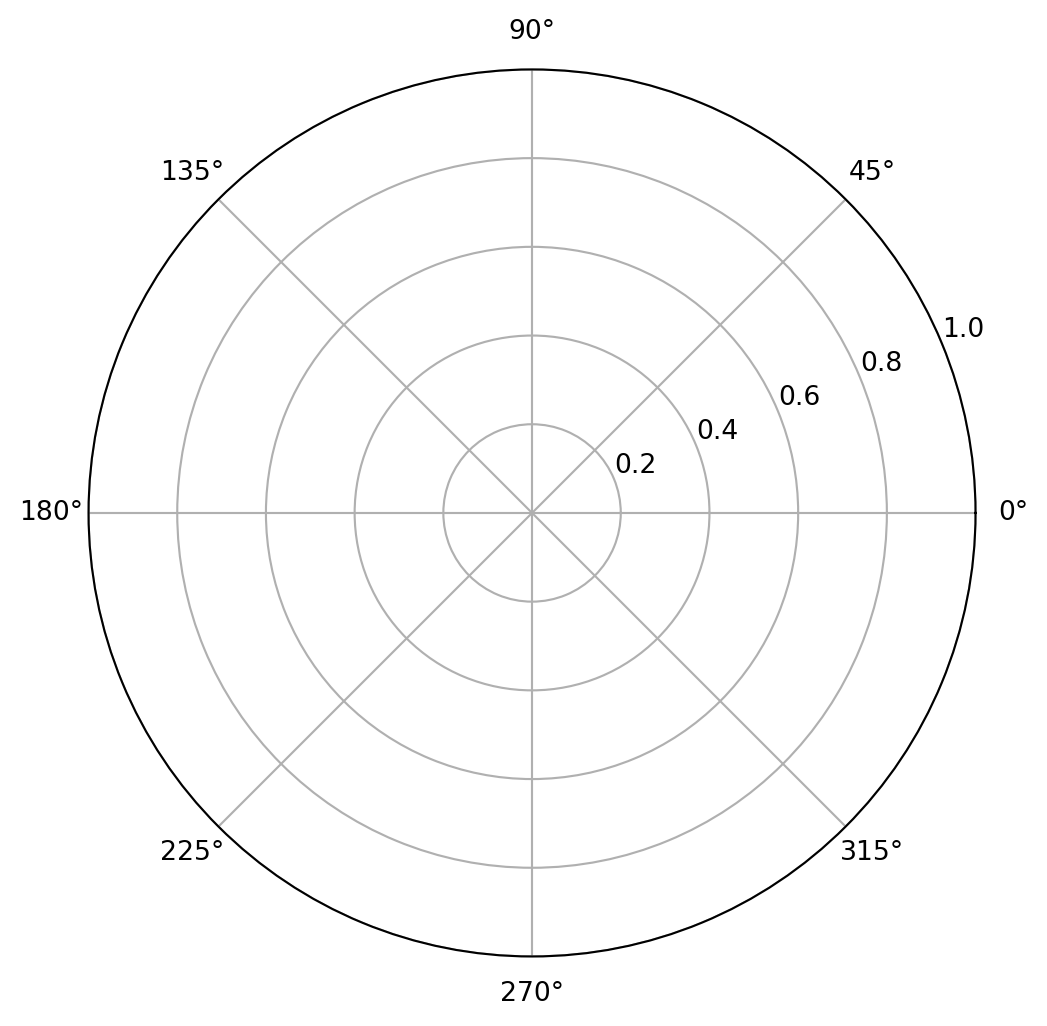
\includegraphics[keepaspectratio]{data-viz_files/figure-pdf/cell-4-output-1.pdf}}

Which is pretty straight forward. There are some nuances within this but
we are just going to keep it pushing.

\section{Adding geometries}\label{adding-geometries}

The next step is to start adding things so we are just going to
initialize a new plot. We kinds of just add things with a dot instead of
a \texttt{+} so lets make a simple scatter plot.

\begin{Shaded}
\begin{Highlighting}[]
\NormalTok{fig,ax }\OperatorTok{=}\NormalTok{ plt.subplots(figsize }\OperatorTok{=}\NormalTok{ (}\DecValTok{6}\NormalTok{,}\DecValTok{6}\NormalTok{))}

\NormalTok{plt.scatter(x }\OperatorTok{=}\NormalTok{ penguins[}\StringTok{\textquotesingle{}bill\_length\_mm\textquotesingle{}}\NormalTok{], y }\OperatorTok{=}\NormalTok{ penguins[}\StringTok{\textquotesingle{}body\_mass\_g\textquotesingle{}}\NormalTok{])}
\end{Highlighting}
\end{Shaded}

\pandocbounded{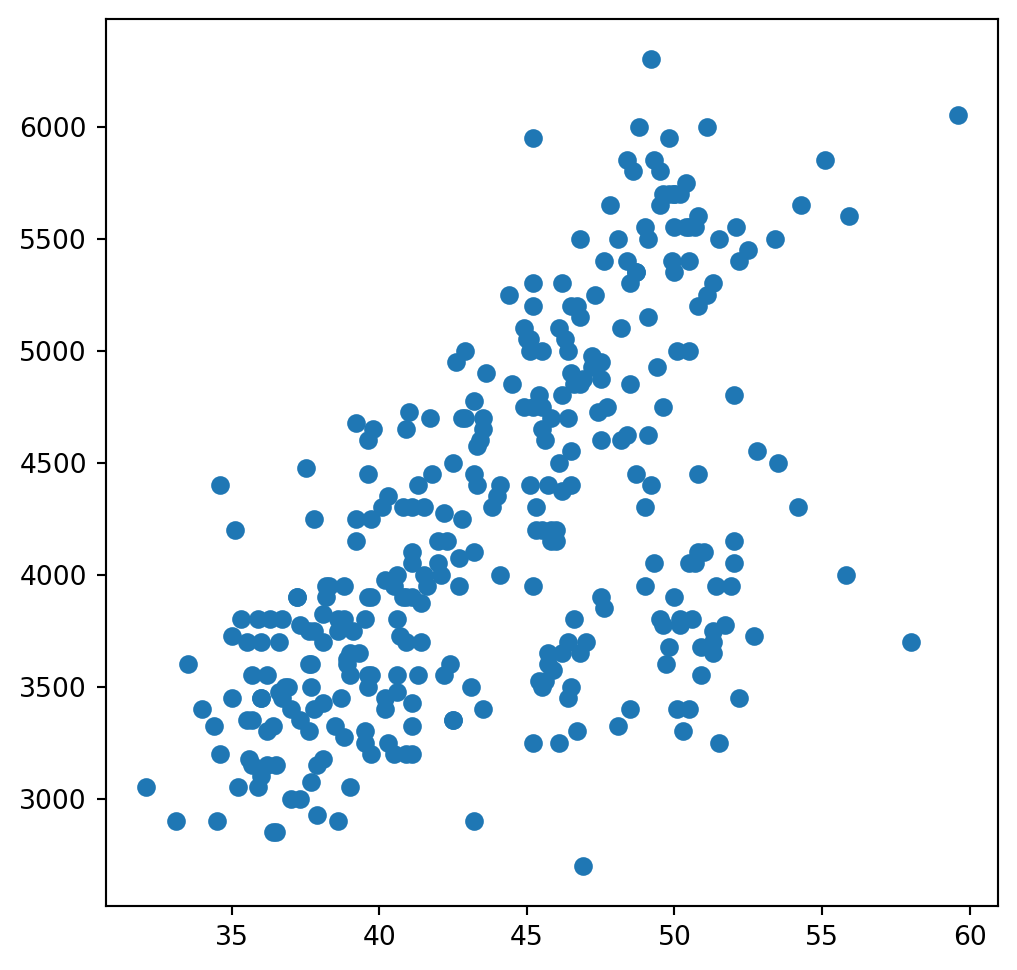
\includegraphics[keepaspectratio]{data-viz_files/figure-pdf/cell-5-output-1.pdf}}

Matplot is a little bit dumber than \texttt{ggplot} meaning that it will
just do exactly what you tell it. So instead of putting basic labels on
the x and y axis like ggplot it will just plot the data. So if we wanted
to add labels to the axis than we need to add the labels

\begin{Shaded}
\begin{Highlighting}[]
\NormalTok{plt.xlabel(}\StringTok{\textquotesingle{}Bill Depth(mm)\textquotesingle{}}\NormalTok{)}

\NormalTok{plt.ylabel(}\StringTok{\textquotesingle{}Body Mass (g)\textquotesingle{}}\NormalTok{)}

\NormalTok{plt.close()}
\end{Highlighting}
\end{Shaded}

We can also add more geometries like this

\begin{Shaded}
\begin{Highlighting}[]
\ImportTok{import}\NormalTok{ numpy }\ImportTok{as}\NormalTok{ np}
\ImportTok{from}\NormalTok{ statsmodels.nonparametric.smoothers\_lowess }\ImportTok{import}\NormalTok{ lowess}

\NormalTok{x }\OperatorTok{=}\NormalTok{ penguins[}\StringTok{\textquotesingle{}bill\_depth\_mm\textquotesingle{}}\NormalTok{].to\_numpy()}

\NormalTok{y }\OperatorTok{=}\NormalTok{ penguins[}\StringTok{\textquotesingle{}body\_mass\_g\textquotesingle{}}\NormalTok{].to\_numpy()}
\NormalTok{smoothed }\OperatorTok{=}\NormalTok{ lowess(y, x, frac}\OperatorTok{=}\FloatTok{0.3}\NormalTok{)  }\CommentTok{\# Adjust \textasciigrave{}frac\textasciigrave{} for smoothing degree}
\NormalTok{x\_smooth }\OperatorTok{=}\NormalTok{ smoothed[:, }\DecValTok{0}\NormalTok{]}
\NormalTok{y\_smooth }\OperatorTok{=}\NormalTok{ smoothed[:, }\DecValTok{1}\NormalTok{]}

\NormalTok{plt.scatter(x, y)}

\NormalTok{plt.plot(x\_smooth, y\_smooth)}
\NormalTok{plt.xlabel(}\StringTok{\textquotesingle{}Bill Depth (mm)\textquotesingle{}}\NormalTok{)}
\NormalTok{plt.ylabel(}\StringTok{\textquotesingle{}Body Mass (g)\textquotesingle{}}\NormalTok{)}

\NormalTok{plt.close()}
\end{Highlighting}
\end{Shaded}

If we wanted to change the method we could do

\begin{Shaded}
\begin{Highlighting}[]
\ImportTok{from}\NormalTok{ sklearn.linear\_model }\ImportTok{import}\NormalTok{ LinearRegression}
\NormalTok{x\_reshape }\OperatorTok{=}\NormalTok{ x.reshape(}\OperatorTok{{-}}\DecValTok{1}\NormalTok{,}\DecValTok{1}\NormalTok{)}

\NormalTok{model }\OperatorTok{=}\NormalTok{ LinearRegression()}

\NormalTok{model.fit(x\_reshape, y }\OperatorTok{=}\NormalTok{ y)}

\NormalTok{y\_pred }\OperatorTok{=}\NormalTok{ model.predict(x\_reshape)}




\NormalTok{plt.scatter(x, y, s}\OperatorTok{=}\DecValTok{10}\NormalTok{, alpha}\OperatorTok{=}\FloatTok{0.7}\NormalTok{, label}\OperatorTok{=}\StringTok{"Original Data"}\NormalTok{)}
\NormalTok{plt.plot(x, y\_pred, color}\OperatorTok{=}\StringTok{"red"}\NormalTok{, label}\OperatorTok{=}\StringTok{"Linear Regression"}\NormalTok{)}
\NormalTok{plt.xlabel(}\StringTok{"Bill Length (mm)"}\NormalTok{)}
\NormalTok{plt.ylabel(}\StringTok{"Body Mass (g)"}\NormalTok{)}
\NormalTok{plt.title(}\StringTok{"Linear Regression: Bill Length vs Body Mass"}\NormalTok{)}
\NormalTok{plt.close()}
\end{Highlighting}
\end{Shaded}

So the pattern emerges that we have some differences based on subgroups.
So we need to plot these by species and then fit a regression line. In
ggplot this process is a little bit more compact. But for matplot it is
a lot like base R where we loop over and then do this.

\begin{Shaded}
\begin{Highlighting}[]
\NormalTok{species\_unique }\OperatorTok{=}\NormalTok{ penguins.unique(subset}\OperatorTok{=}\StringTok{\textquotesingle{}species\textquotesingle{}}\NormalTok{).sort(}\StringTok{\textquotesingle{}species\textquotesingle{}}\NormalTok{)[}\StringTok{\textquotesingle{}species\textquotesingle{}}\NormalTok{]}

\NormalTok{penguins.glimpse()}

\NormalTok{markers }\OperatorTok{=}\NormalTok{ [}\StringTok{\textquotesingle{}o\textquotesingle{}}\NormalTok{, }\StringTok{\textquotesingle{}s\textquotesingle{}}\NormalTok{, }\StringTok{\textquotesingle{}\^{}\textquotesingle{}}\NormalTok{]}

\NormalTok{colors }\OperatorTok{=}\NormalTok{ [}\StringTok{\textquotesingle{}red\textquotesingle{}}\NormalTok{, }\StringTok{\textquotesingle{}blue\textquotesingle{}}\NormalTok{, }\StringTok{\textquotesingle{}green\textquotesingle{}}\NormalTok{]}

\ControlFlowTok{for}\NormalTok{ species, marker, color }\KeywordTok{in} \BuiltInTok{zip}\NormalTok{(species\_unique, markers, colors):}
\NormalTok{    species\_data }\OperatorTok{=}\NormalTok{ penguins.}\BuiltInTok{filter}\NormalTok{(pl.col(}\StringTok{\textquotesingle{}species\textquotesingle{}}\NormalTok{) }\OperatorTok{==}\NormalTok{ species)}
\NormalTok{    plt.scatter(x }\OperatorTok{=}\NormalTok{ species\_data[}\StringTok{\textquotesingle{}bill\_length\_mm\textquotesingle{}}\NormalTok{], y }\OperatorTok{=}\NormalTok{ species\_data[}\StringTok{\textquotesingle{}bill\_depth\_mm\textquotesingle{}}\NormalTok{],}
\NormalTok{    label }\OperatorTok{=}\NormalTok{ species, marker }\OperatorTok{=}\NormalTok{ marker, color }\OperatorTok{=}\NormalTok{ color )}
\NormalTok{    plt.xlabel(}\StringTok{\textquotesingle{}Bill Length (mm)\textquotesingle{}}\NormalTok{)}
\NormalTok{    plt.ylabel(}\StringTok{\textquotesingle{}Bill Depth (mm)\textquotesingle{}}\NormalTok{)}
\NormalTok{    plt.legend()}
\end{Highlighting}
\end{Shaded}

\begin{verbatim}
Rows: 333
Columns: 8
$ species           <str> 'Adelie', 'Adelie', 'Adelie', 'Adelie', 'Adelie', 'Adelie', 'Adelie', 'Adelie', 'Adelie', 'Adelie'
$ island            <str> 'Torgersen', 'Torgersen', 'Torgersen', 'Torgersen', 'Torgersen', 'Torgersen', 'Torgersen', 'Torgersen', 'Torgersen', 'Torgersen'
$ bill_length_mm    <f64> 39.1, 39.5, 40.3, 36.7, 39.3, 38.9, 39.2, 41.1, 38.6, 34.6
$ bill_depth_mm     <f64> 18.7, 17.4, 18.0, 19.3, 20.6, 17.8, 19.6, 17.6, 21.2, 21.1
$ flipper_length_mm <f64> 181.0, 186.0, 195.0, 193.0, 190.0, 181.0, 195.0, 182.0, 191.0, 198.0
$ body_mass_g       <f64> 3750.0, 3800.0, 3250.0, 3450.0, 3650.0, 3625.0, 4675.0, 3200.0, 3800.0, 4400.0
$ sex               <str> 'male', 'female', 'female', 'female', 'male', 'female', 'male', 'female', 'male', 'male'
$ year              <i64> 2007, 2007, 2007, 2007, 2007, 2007, 2007, 2007, 2007, 2007
\end{verbatim}

\pandocbounded{\includegraphics[keepaspectratio]{data-viz_files/figure-pdf/cell-9-output-2.pdf}}

In a similar way we need to do this for the the linear regression lines

\begin{Shaded}
\begin{Highlighting}[]
\ControlFlowTok{for}\NormalTok{ species, marker, color }\KeywordTok{in} \BuiltInTok{zip}\NormalTok{(species\_unique, markers, colors):}
    \CommentTok{\# Filter data for the current species}
\NormalTok{    species\_data }\OperatorTok{=}\NormalTok{ penguins.}\BuiltInTok{filter}\NormalTok{(pl.col(}\StringTok{\textquotesingle{}species\textquotesingle{}}\NormalTok{) }\OperatorTok{==}\NormalTok{ species)}

    \CommentTok{\# Extract x and y values}
\NormalTok{    x }\OperatorTok{=}\NormalTok{ species\_data[}\StringTok{\textquotesingle{}bill\_length\_mm\textquotesingle{}}\NormalTok{].to\_numpy()}
\NormalTok{    y }\OperatorTok{=}\NormalTok{ species\_data[}\StringTok{\textquotesingle{}bill\_depth\_mm\textquotesingle{}}\NormalTok{].to\_numpy()}

    \CommentTok{\# Scatter plot}
\NormalTok{    plt.scatter(x, y, label}\OperatorTok{=}\NormalTok{species, marker}\OperatorTok{=}\NormalTok{marker, color}\OperatorTok{=}\NormalTok{color)}

    \CommentTok{\# Fit linear regression (1st{-}degree polynomial)}
\NormalTok{    m, b }\OperatorTok{=}\NormalTok{ np.polyfit(x, y, }\DecValTok{1}\NormalTok{)}

    \CommentTok{\# Plot regression line}
\NormalTok{    plt.plot(x, m }\OperatorTok{*}\NormalTok{ x }\OperatorTok{+}\NormalTok{ b, color}\OperatorTok{=}\NormalTok{color)}

\CommentTok{\# Add labels and legend}
\NormalTok{plt.xlabel(}\StringTok{\textquotesingle{}Bill Length (mm)\textquotesingle{}}\NormalTok{)}
\NormalTok{plt.ylabel(}\StringTok{\textquotesingle{}Bill Depth (mm)\textquotesingle{}}\NormalTok{)}
\NormalTok{plt.legend()}
\NormalTok{plt.show()}
\end{Highlighting}
\end{Shaded}

\pandocbounded{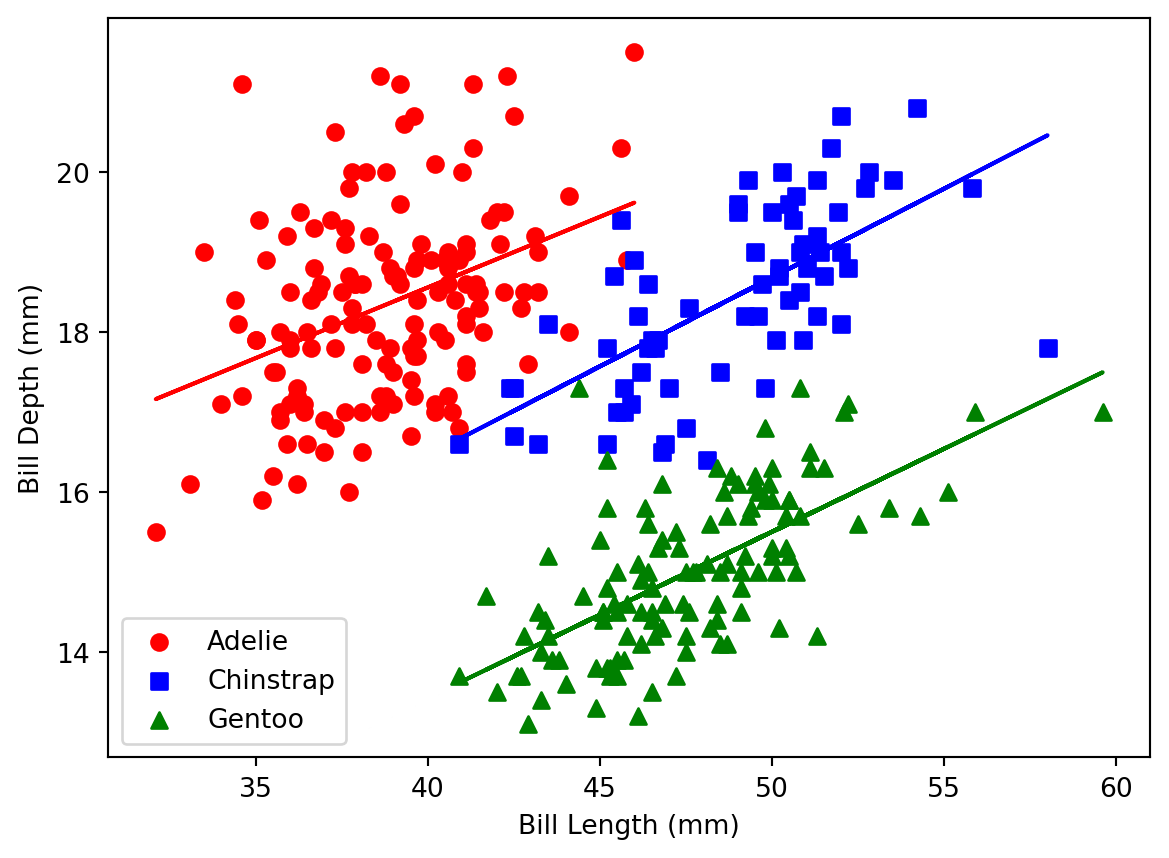
\includegraphics[keepaspectratio]{data-viz_files/figure-pdf/cell-11-output-1.pdf}}

\bookmarksetup{startatroot}

\chapter{Probability}\label{probability}

We have our general sense of probabilities where we are just the number
of times things occur. This is kind of helpful.

\begin{Shaded}
\begin{Highlighting}[]
\ImportTok{import}\NormalTok{ numpy }\ImportTok{as}\NormalTok{ np}
\ImportTok{from}\NormalTok{ scipy }\ImportTok{import}\NormalTok{ stats }\ImportTok{as}\NormalTok{ stats }
\ImportTok{from}\NormalTok{ matplotlib }\ImportTok{import}\NormalTok{ pyplot }\ImportTok{as}\NormalTok{ plt}
\ImportTok{import}\NormalTok{ polars }\ImportTok{as}\NormalTok{ pl}

\NormalTok{numbs }\OperatorTok{=}\NormalTok{ np.array([}\DecValTok{1}\NormalTok{,}\DecValTok{3}\NormalTok{,}\DecValTok{4}\NormalTok{,}\DecValTok{3}\NormalTok{])}

\DecValTok{1}\OperatorTok{/}\NormalTok{numbs.}\BuiltInTok{sum}\NormalTok{()}
\end{Highlighting}
\end{Shaded}

\begin{verbatim}
0.09090909090909091
\end{verbatim}

However, for the most part in the real world we don't neccessarily care
about the probability of a single event happening unconditionally.
Conditioanl probability is genereallly a little weird but not totally
different than just counting.

\section{Conditional Probability}\label{conditional-probability}

There are two ways we generally think of basic condiitonal probability
Frequentistly and Bayesianly. For the most part these are fairly
similar. The key difference is how we incorporate what we know about the
world.

\subsection{Freqeuentist}\label{freqeuentist}

In Frequentism people often say that we don't impose any priors on the
data. This is not true in any real sense because we impose a flat prior.
So the prior is kind of incorporated for us. Typically we see
conditional probabilities expressed in two ways

\[
\text{P(A|B)} = \frac{\text{Probability of A and B Hapenning}}{\text{Probability of B happening}} \\\
\text{P(A|B)} = \frac{\text{P(A)} \cap \text{P(B)}}{\text{P(B)}} 
\]

This is a bit hard to visualize so lets take an example

\begin{Shaded}
\begin{Highlighting}[]
\NormalTok{senators.glimpse()}
\end{Highlighting}
\end{Shaded}

\begin{verbatim}
Rows: 6
Columns: 3
$ party  <str> 'Democrats', 'Republican', 'Independents', 'Democrats', 'Republican', 'Independents'
$ gender <str> 'Men', 'Men', 'Men', 'Woman', 'Woman', 'Woman'
$ total  <i64> 33, 40, 2, 15, 9, 1
\end{verbatim}

So if we wanted to calculate the conditional probability of drawing a
female democratic senator we would really just do this.

\begin{Shaded}
\begin{Highlighting}[]
\NormalTok{womand\_democrat }\OperatorTok{=}\NormalTok{ senators.}\BuiltInTok{filter}\NormalTok{((pl.col(}\StringTok{\textquotesingle{}gender\textquotesingle{}}\NormalTok{) }\OperatorTok{==} \StringTok{\textquotesingle{}Woman\textquotesingle{}}\NormalTok{) }\OperatorTok{\&}\NormalTok{ (pl.col(}\StringTok{\textquotesingle{}party\textquotesingle{}}\NormalTok{) }\OperatorTok{==} \StringTok{\textquotesingle{}Democrats\textquotesingle{}}\NormalTok{))[}\StringTok{\textquotesingle{}total\textquotesingle{}}\NormalTok{]}

\NormalTok{democrat }\OperatorTok{=}\NormalTok{ senators.}\BuiltInTok{filter}\NormalTok{(pl.col(}\StringTok{\textquotesingle{}party\textquotesingle{}}\NormalTok{) }\OperatorTok{==} \StringTok{\textquotesingle{}Democrats\textquotesingle{}}\NormalTok{).with\_columns(total }\OperatorTok{=}\NormalTok{ pl.col(}\StringTok{\textquotesingle{}total\textquotesingle{}}\NormalTok{).}\BuiltInTok{sum}\NormalTok{())[}\StringTok{\textquotesingle{}total\textquotesingle{}}\NormalTok{][}\DecValTok{0}\NormalTok{]}

\NormalTok{denom }\OperatorTok{=} \DecValTok{100}

\NormalTok{(womand\_democrat}\OperatorTok{/}\DecValTok{100}\NormalTok{)}\OperatorTok{/}\NormalTok{(democrat}\OperatorTok{/}\DecValTok{100}\NormalTok{)}
\end{Highlighting}
\end{Shaded}

\begin{longtable}[]{@{}l@{}}
\toprule\noalign{}
total \\
f64 \\
\midrule\noalign{}
\endhead
\bottomrule\noalign{}
\endlastfoot
0.3125 \\
\end{longtable}

So this will roughly get us that the odds of drawing a female democratic
senator is 0.31.

\subsection{Bayesianism}\label{bayesianism}

Bayesians view conditional probability in a slightly different way. But
as Richard McCelreath argues that isn't entirely true in this canned
example. Typically we define Bayes Rule as something along these lines.

\begin{align}

\text{P(A|B)} = \frac{\text{P(A and B)} \times \text{P(B)}}{P(A)}

\end{align}

However, that is not all that interesting because we when we plug in
numbers like we would in a frequentist setting because our we will start
updating as we see more data. The canoncial example is some sort of
testing framework. In statistical rethinking they use ``Vampirism''

\begin{Shaded}
\begin{Highlighting}[]
\NormalTok{prob\_vampire\_positive }\OperatorTok{=} \FloatTok{0.95} 

\NormalTok{prob\_positive\_mortal }\OperatorTok{=} \FloatTok{0.01}

\NormalTok{pr\_vamp }\OperatorTok{=} \FloatTok{0.001} 

\NormalTok{pr\_positive }\OperatorTok{=}\NormalTok{ prob\_vampire\_positive }\OperatorTok{*}\NormalTok{ pr\_vamp }\OperatorTok{+}\NormalTok{ prob\_positive\_mortal }\OperatorTok{*}\NormalTok{ (}\DecValTok{1}\OperatorTok{{-}}\NormalTok{pr\_vamp)}

\NormalTok{prob\_vampire\_positive }\OperatorTok{*}\NormalTok{ pr\_vamp }\OperatorTok{/}\NormalTok{  pr\_positive}
\end{Highlighting}
\end{Shaded}

\begin{verbatim}
0.08683729433272395
\end{verbatim}

However as Rich points out there is nothing uniquely Bayesian about this
example. We could theoretically rewrite this to just plug in the numbers
into the classic frequentist conditional probability statement.

What makes Bayesianism interesting is when we start updating the
posterior distribution. Under the hood we need integral calculus to do
this but hand deriving that either on paper or from scratch. Really what
we are kind of doing when we run this through a MCMC is that we are
sampling from our posterior distribution and counting the frequencies
that something occurs. I am going to use the counting water example

\begin{Shaded}
\begin{Highlighting}[]
\KeywordTok{def}\NormalTok{ calculate\_n\_ways\_possible(observations: }\BuiltInTok{str}\NormalTok{, n\_water: }\BuiltInTok{int}\NormalTok{, resolution: }\BuiltInTok{int} \OperatorTok{=} \DecValTok{4}\NormalTok{):}
    \CommentTok{"""}
\CommentTok{    Calculate the number of ways to observing water (\textquotesingle{}W\textquotesingle{}) given the toss of a globe}
\CommentTok{    with \textasciigrave{}resolution\textasciigrave{} number of sides and \textasciigrave{}n\_water\textasciigrave{} faces.}
\CommentTok{    }
\CommentTok{    Note: this method results in numerical precision issues (due to the product) when the}
\CommentTok{    resolution of 16 or so, depending on your system.}
\CommentTok{    """}
    \ControlFlowTok{assert}\NormalTok{ n\_water }\OperatorTok{\textless{}=}\NormalTok{ resolution}
    
    \CommentTok{\# Convert observation string to an array}
\NormalTok{    observations }\OperatorTok{=}\NormalTok{ np.array(}\BuiltInTok{list}\NormalTok{(observations.upper()))}
    
    \CommentTok{\# Create n{-}sided globe with possible outcomes}
\NormalTok{    possible }\OperatorTok{=}\NormalTok{ np.array(}\BuiltInTok{list}\NormalTok{(}\StringTok{"L"} \OperatorTok{*}\NormalTok{ (resolution }\OperatorTok{{-}}\NormalTok{ n\_water)) }\OperatorTok{+} \BuiltInTok{list}\NormalTok{(}\StringTok{"W"} \OperatorTok{*}\NormalTok{ n\_water))}
    
    \CommentTok{\# Tally up ways to obtain each observation given the possible outcomes}
    \CommentTok{\# Here we use brute{-}force, but we could also use the analytical solution below}
\NormalTok{    ways }\OperatorTok{=}\NormalTok{ []}
    \ControlFlowTok{for}\NormalTok{ obs }\KeywordTok{in}\NormalTok{ observations:}
\NormalTok{        ways.append((possible }\OperatorTok{==}\NormalTok{ obs).}\BuiltInTok{sum}\NormalTok{())}
    
\NormalTok{    p\_water }\OperatorTok{=}\NormalTok{ n\_water }\OperatorTok{/}\NormalTok{ resolution}
    \CommentTok{\# perform product in log space for numerical precision}
\NormalTok{    n\_ways }\OperatorTok{=}\NormalTok{ np.}\BuiltInTok{round}\NormalTok{(np.exp(np.}\BuiltInTok{sum}\NormalTok{(np.log(ways)))).astype(}\BuiltInTok{int}\NormalTok{)}
    \ControlFlowTok{return}\NormalTok{ n\_ways, p\_water}


\KeywordTok{def}\NormalTok{ run\_globe\_tossing\_simulation(observations, resolution, current\_n\_possible\_ways}\OperatorTok{=}\VariableTok{None}\NormalTok{):}
    \CommentTok{"""Simulate the number of ways you can observe water (\textquotesingle{}W\textquotesingle{}) for a globe of \textasciigrave{}resolution\textasciigrave{}}
\CommentTok{    sides, varying the proportion of the globe that is covered by water.}
\CommentTok{    """}
    \CommentTok{\# For Bayesian updates}
\NormalTok{    current\_n\_possible\_ways }\OperatorTok{=}\NormalTok{ current\_n\_possible\_ways }\ControlFlowTok{if}\NormalTok{ current\_n\_possible\_ways }\KeywordTok{is} \KeywordTok{not} \VariableTok{None} \ControlFlowTok{else}\NormalTok{ np.array([])}
    
    \BuiltInTok{print}\NormalTok{(}\SpecialStringTok{f"Observations: \textquotesingle{}}\SpecialCharTok{\{}\NormalTok{observations}\SpecialCharTok{\}}\SpecialStringTok{\textquotesingle{}"}\NormalTok{)}
\NormalTok{    p\_water }\OperatorTok{=}\NormalTok{ np.array([])}
    \ControlFlowTok{for}\NormalTok{ n\_W }\KeywordTok{in} \BuiltInTok{range}\NormalTok{(}\DecValTok{0}\NormalTok{, resolution }\OperatorTok{+} \DecValTok{1}\NormalTok{):}
\NormalTok{        n\_L }\OperatorTok{=}\NormalTok{ resolution }\OperatorTok{{-}}\NormalTok{ n\_W}
\NormalTok{        globe\_sides }\OperatorTok{=} \StringTok{"W"} \OperatorTok{*}\NormalTok{ n\_W }\OperatorTok{+} \StringTok{"L"} \OperatorTok{*}\NormalTok{ n\_L}
\NormalTok{        n\_possible\_ways, p\_water\_ }\OperatorTok{=}\NormalTok{ calculate\_n\_ways\_possible(observations, n\_water}\OperatorTok{=}\NormalTok{n\_W, resolution}\OperatorTok{=}\NormalTok{resolution)}
        \BuiltInTok{print}\NormalTok{(}\SpecialStringTok{f"(}\SpecialCharTok{\{}\NormalTok{n\_W}\OperatorTok{+}\DecValTok{1}\SpecialCharTok{\}}\SpecialStringTok{) }\SpecialCharTok{\{}\NormalTok{globe\_sides}\SpecialCharTok{\}}\SpecialStringTok{ p(W) = }\SpecialCharTok{\{}\NormalTok{p\_water\_}\SpecialCharTok{:1.2\}}\CharTok{\textbackslash{}t\textbackslash{}t}\SpecialCharTok{\{}\NormalTok{n\_possible\_ways}\SpecialCharTok{\}}\SpecialStringTok{ Ways to Produce"}\NormalTok{)}

\NormalTok{        p\_water }\OperatorTok{=}\NormalTok{ np.append(p\_water, p\_water\_)}
\NormalTok{        current\_n\_possible\_ways }\OperatorTok{=}\NormalTok{ np.append(current\_n\_possible\_ways, n\_possible\_ways)}

    \ControlFlowTok{return}\NormalTok{ current\_n\_possible\_ways, p\_water}

\ImportTok{from}\NormalTok{ pprint }\ImportTok{import}\NormalTok{ pprint}
\NormalTok{np.random.seed(}\DecValTok{1}\NormalTok{)}
\KeywordTok{def}\NormalTok{ simulate\_globe\_toss(p: }\BuiltInTok{float} \OperatorTok{=} \FloatTok{0.7}\NormalTok{, N: }\BuiltInTok{int} \OperatorTok{=} \DecValTok{9}\NormalTok{) }\OperatorTok{{-}\textgreater{}} \BuiltInTok{list}\NormalTok{[}\BuiltInTok{str}\NormalTok{]:}
    \CommentTok{"""Simulate N globe tosses with a specific/known proportion}
\CommentTok{    p: float}
\CommentTok{        The propotion of water}
\CommentTok{    N: int}
\CommentTok{        Number of globe tosses}
\CommentTok{    """}
    \ControlFlowTok{return}\NormalTok{ np.random.choice(}\BuiltInTok{list}\NormalTok{(}\StringTok{"WL"}\NormalTok{),  size}\OperatorTok{=}\NormalTok{N, p}\OperatorTok{=}\NormalTok{np.array([p, }\DecValTok{1}\OperatorTok{{-}}\NormalTok{p]), replace}\OperatorTok{=}\VariableTok{True}\NormalTok{)}
\end{Highlighting}
\end{Shaded}

\begin{Shaded}
\begin{Highlighting}[]
\NormalTok{RESOLUTION }\OperatorTok{=} \DecValTok{4}
\NormalTok{observations }\OperatorTok{=} \StringTok{"WLW"}
\NormalTok{n\_possible\_ways, p\_water }\OperatorTok{=}\NormalTok{ run\_globe\_tossing\_simulation(observations, resolution}\OperatorTok{=}\NormalTok{RESOLUTION)}
\end{Highlighting}
\end{Shaded}

\begin{verbatim}
Observations: 'WLW'
(1) LLLL p(W) = 0.0     0 Ways to Produce
(2) WLLL p(W) = 0.25        3 Ways to Produce
(3) WWLL p(W) = 0.5     8 Ways to Produce
(4) WWWL p(W) = 0.75        9 Ways to Produce
(5) WWWW p(W) = 1.0     0 Ways to Produce
\end{verbatim}

This will spit out the number of ways we can produce various draws. Now
lets simulate the number of globe tosses wher we are just adding tosses.

\begin{Shaded}
\begin{Highlighting}[]
\ImportTok{from}\NormalTok{ scipy.special }\ImportTok{import}\NormalTok{ factorial}

\KeywordTok{def}\NormalTok{ beta\_posterior(n\_W: }\BuiltInTok{int}\NormalTok{, n\_L: }\BuiltInTok{int}\NormalTok{, p: }\BuiltInTok{float}\NormalTok{) }\OperatorTok{{-}\textgreater{}} \BuiltInTok{float}\NormalTok{:}
    \CommentTok{"""Calculates the beta posterior over proportions \textasciigrave{}p\textasciigrave{} given a set of}
\CommentTok{    \textasciigrave{}N\_W\textasciigrave{} water and \textasciigrave{}N\_L\textasciigrave{} land observations}
\CommentTok{    """}
    \ControlFlowTok{return}\NormalTok{ factorial(n\_W }\OperatorTok{+}\NormalTok{ n\_L }\OperatorTok{+} \DecValTok{1}\NormalTok{) }\OperatorTok{/}\NormalTok{ (factorial(n\_W) }\OperatorTok{*}\NormalTok{ factorial(n\_L)) }\OperatorTok{*}\NormalTok{ p }\OperatorTok{**}\NormalTok{ n\_W }\OperatorTok{*}\NormalTok{ (}\DecValTok{1}\OperatorTok{{-}}\NormalTok{p) }\OperatorTok{**}\NormalTok{ n\_L}


\KeywordTok{def}\NormalTok{ plot\_beta\_posterior\_from\_observations(observations: }\BuiltInTok{str}\NormalTok{, resolution: }\BuiltInTok{int} \OperatorTok{=} \DecValTok{50}\NormalTok{, }\OperatorTok{**}\NormalTok{plot\_kwargs) }\OperatorTok{{-}\textgreater{}} \VariableTok{None}\NormalTok{:}
    \CommentTok{"""Calculates and plots the beta posterior for a string of observations"""}
\NormalTok{    n\_W }\OperatorTok{=} \BuiltInTok{len}\NormalTok{(observations.replace(}\StringTok{"L"}\NormalTok{, }\StringTok{""}\NormalTok{))}
\NormalTok{    n\_L }\OperatorTok{=} \BuiltInTok{len}\NormalTok{(observations) }\OperatorTok{{-}}\NormalTok{ n\_W}
\NormalTok{    proportions }\OperatorTok{=}\NormalTok{ np.linspace(}\DecValTok{0}\NormalTok{, }\DecValTok{1}\NormalTok{, resolution)}
        
\NormalTok{    probs }\OperatorTok{=}\NormalTok{ beta\_posterior(n\_W, n\_L, proportions)}
\NormalTok{    plt.plot(proportions, probs, }\OperatorTok{**}\NormalTok{plot\_kwargs)}
\NormalTok{    plt.yticks([])}
\NormalTok{    plt.title(observations)}
    

\CommentTok{\# Tossing the globe}
\NormalTok{observations }\OperatorTok{=} \StringTok{"WLWWWLWLW"}
\NormalTok{fig, axs }\OperatorTok{=}\NormalTok{ plt.subplots(}\DecValTok{3}\NormalTok{, }\DecValTok{3}\NormalTok{, figsize}\OperatorTok{=}\NormalTok{(}\DecValTok{8}\NormalTok{, }\DecValTok{8}\NormalTok{))}
\ControlFlowTok{for}\NormalTok{ ii }\KeywordTok{in} \BuiltInTok{range}\NormalTok{(}\DecValTok{9}\NormalTok{):}
\NormalTok{    ax }\OperatorTok{=}\NormalTok{ axs[ii }\OperatorTok{//} \DecValTok{3}\NormalTok{][ii }\OperatorTok{\%} \DecValTok{3}\NormalTok{]}
\NormalTok{    plt.sca(ax)}
    \CommentTok{\# Plot previous}
    \ControlFlowTok{if}\NormalTok{ ii }\OperatorTok{\textgreater{}} \DecValTok{0}\NormalTok{:}
\NormalTok{        plot\_beta\_posterior\_from\_observations(observations[:ii], color}\OperatorTok{=}\StringTok{\textquotesingle{}k\textquotesingle{}}\NormalTok{, linestyle}\OperatorTok{=}\StringTok{\textquotesingle{}{-}{-}\textquotesingle{}}\NormalTok{)}
    \ControlFlowTok{else}\NormalTok{:}
        \CommentTok{\# First observation, no previous data}
\NormalTok{        plot\_beta\_posterior\_from\_observations(}\StringTok{\textquotesingle{}\textquotesingle{}}\NormalTok{, color}\OperatorTok{=}\StringTok{\textquotesingle{}k\textquotesingle{}}\NormalTok{, linestyle}\OperatorTok{=}\StringTok{\textquotesingle{}{-}{-}\textquotesingle{}}\NormalTok{)}
        
\NormalTok{    color }\OperatorTok{=} \StringTok{\textquotesingle{}C1\textquotesingle{}} \ControlFlowTok{if}\NormalTok{ observations[ii] }\OperatorTok{==} \StringTok{\textquotesingle{}W\textquotesingle{}} \ControlFlowTok{else} \StringTok{\textquotesingle{}C0\textquotesingle{}}
\NormalTok{    plot\_beta\_posterior\_from\_observations(observations[:ii}\OperatorTok{+}\DecValTok{1}\NormalTok{], color}\OperatorTok{=}\NormalTok{color, linewidth}\OperatorTok{=}\DecValTok{4}\NormalTok{, alpha}\OperatorTok{=}\FloatTok{.5}\NormalTok{)}
    
    \ControlFlowTok{if} \KeywordTok{not}\NormalTok{ ii }\OperatorTok{\%} \DecValTok{3}\NormalTok{:}
\NormalTok{        plt.ylabel(}\StringTok{"posterior probability"}\NormalTok{)}
\end{Highlighting}
\end{Shaded}

\pandocbounded{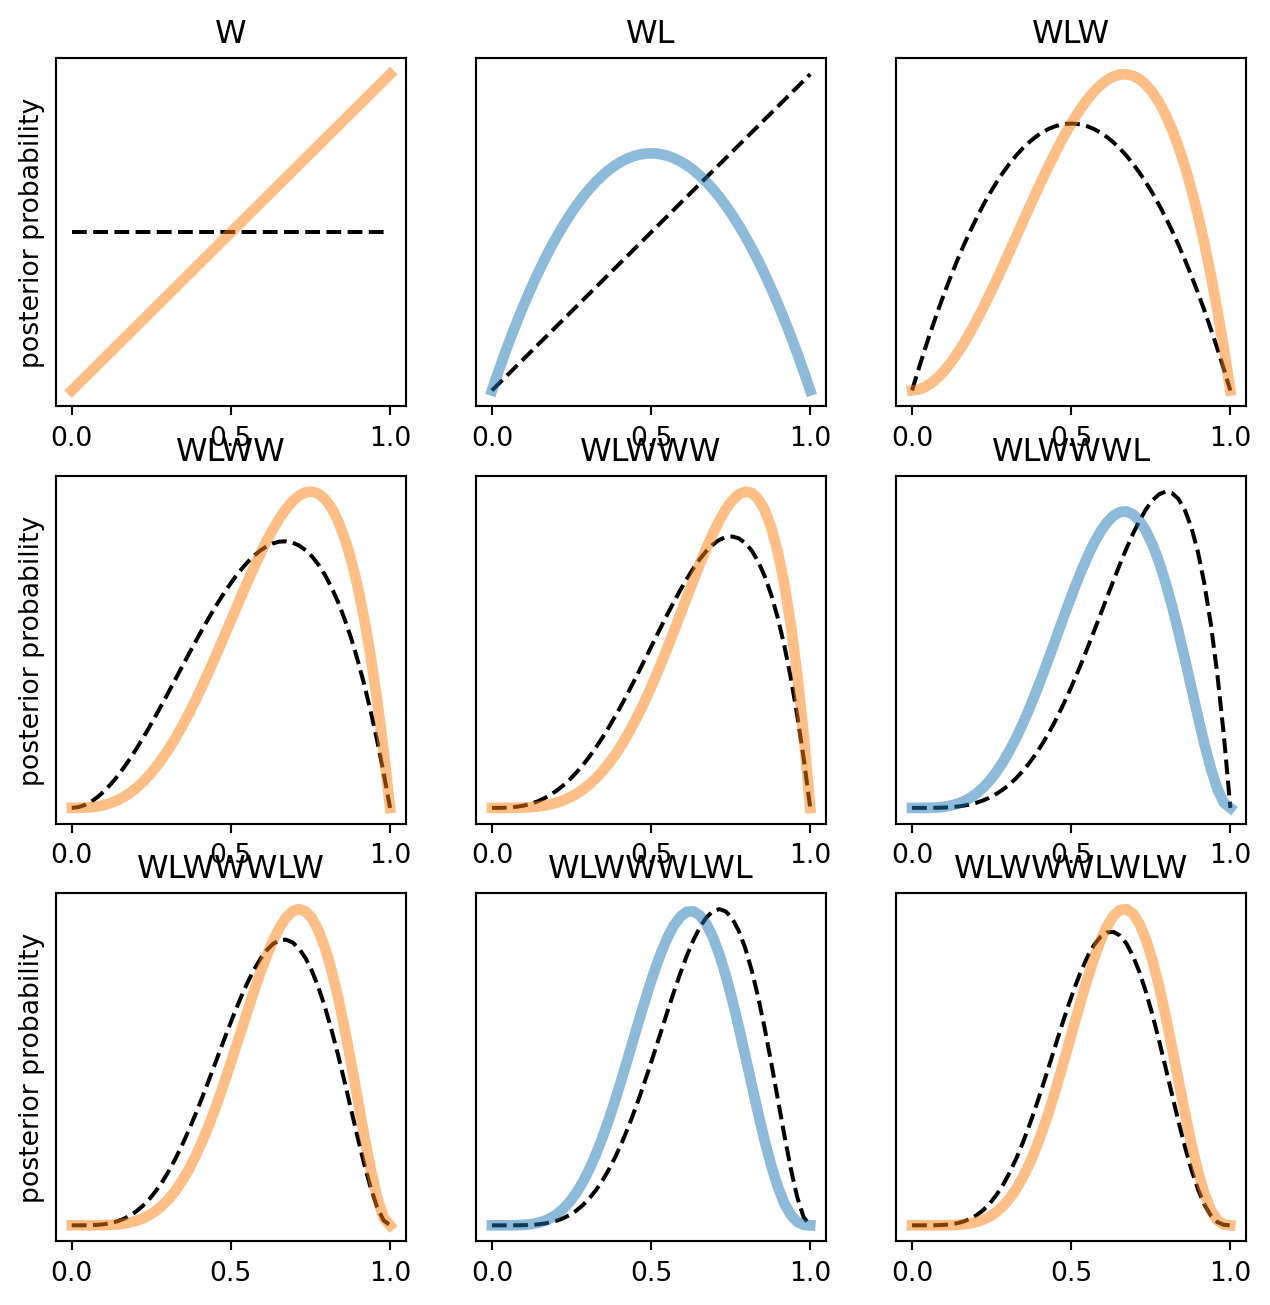
\includegraphics[keepaspectratio]{probability_files/figure-pdf/cell-9-output-1.pdf}}

\section{Counting}\label{counting}

One component of interviews is that we should have some intuition on
counting. Like not 1,2,3 etc but how many possible combinations of
things can there be aka permutations and combinations. It has been
awhile since you have had to do this so it is worth going over.
Permutations care about about the unique order that things can be paired
in. While combinations are order agnostic. Lets say that we are trying
to figure out the number of possible ways that we can seat guests at
various tables. That would be a combination. For your own sake lets
number all the seats. A permutation would care about the number of
unique ways we can arrange people while taking the seat numbers
available. What is underriding this whole thing is factorials and
orders. So the formulas look something like this. Where n is the number
of items and k is the number of items to arrange

\begin{align}
\text{permutation} = \frac{n!}{(n-k)!} \\

\text{combination} = \frac{n!}{k!(n-k)!}

\end{align}

factorials are just a simplfying way of writing out something like this.
Where we are progresively multiplying 1 by 1 to 2 * 1 then so on and so
forth.

\begin{Shaded}
\begin{Highlighting}[]
\KeywordTok{def}\NormalTok{ factorial(n):}

\NormalTok{    result }\OperatorTok{=} \DecValTok{1}
    \ControlFlowTok{for}\NormalTok{ i }\KeywordTok{in} \BuiltInTok{range}\NormalTok{(}\DecValTok{1}\NormalTok{, n }\OperatorTok{+} \DecValTok{1}\NormalTok{):}
\NormalTok{        result }\OperatorTok{*=}\NormalTok{ i}
    \ControlFlowTok{return}\NormalTok{ result}

\BuiltInTok{print}\NormalTok{(factorial(n }\OperatorTok{=} \DecValTok{5}\NormalTok{))}
\end{Highlighting}
\end{Shaded}

\begin{verbatim}
120
\end{verbatim}

Lets say we wanted to figure out the number of possible table
combinations. Lets say we have 20 people and 5 tables. So we would do
something like this.

\begin{Shaded}
\begin{Highlighting}[]
\ImportTok{import}\NormalTok{ math }

\NormalTok{math.factorial(}\DecValTok{20}\NormalTok{)}\OperatorTok{//}\NormalTok{(math.factorial(}\DecValTok{5}\NormalTok{) }\OperatorTok{*}\NormalTok{ math.factorial(}\DecValTok{20} \OperatorTok{{-}} \DecValTok{5}\NormalTok{))}
\end{Highlighting}
\end{Shaded}

\begin{verbatim}
15504
\end{verbatim}

However this is not really how wedding seating works. Order matters and
who sits next to who matters. So we need to take that into account. In
instead of multiplying by the factorial of k we do something like this
with permutations

\begin{Shaded}
\begin{Highlighting}[]
\NormalTok{math.factorial(}\DecValTok{20}\NormalTok{)}\OperatorTok{//}\NormalTok{(factorial(}\DecValTok{20}\OperatorTok{{-}}\DecValTok{5}\NormalTok{))}
\end{Highlighting}
\end{Shaded}

\begin{verbatim}
1860480
\end{verbatim}

\section{The Centeral Limit Theorum}\label{the-centeral-limit-theorum}

She is genuinely one of the most coolest concepts in statistics.
Bascially no matter the distribution of the variablee as we take more
and more samples of the data as N increases we are going to converge to
a normal distribution. This is really powerful concept in frequentist
statistics because we are making inferences about the population using
samples.

\section{Explain the Difference Between Probability and
Likelihood}\label{explain-the-difference-between-probability-and-likelihood}

Probability and likelihood are two concepts that are often used in
statistics and data analysis, but they have different meanings and uses.

Probability is the measure of the likelihood of an event occurring. It
is a number between 0 and 1, with 0 indicating an impossible event and 1
indicating a certain event. For example, the probability of flipping a
coin and getting heads is 0.5.

The likelihood, on the other hand, is the measure of how well a
statistical model or hypothesis fits a set of observed data. It is not a
probability, but rather a measure of how plausible the data is given the
model or hypothesis. For example, if we have a hypothesis that the
average height of people in a certain population is 6 feet, the
likelihood of observing a random sample of people with an average height
of 5 feet would be low.

\bookmarksetup{startatroot}

\chapter{Linear Regression and Shrinkage
Estimators}\label{linear-regression-and-shrinkage-estimators}

Since the bulk of your work will be building machnine learning models it
is probably going to be important that you get way more comfortable with
machine learning in python. You are a bit of a unicorn in the sense that
you will do anything but learn pandas. So you are going to have to make
sure that this isn't new information.

\begin{Shaded}
\begin{Highlighting}[]
\ImportTok{import}\NormalTok{ polars }\ImportTok{as}\NormalTok{ pl }
\ImportTok{import}\NormalTok{ numpy }\ImportTok{as}\NormalTok{ np}
\ImportTok{import}\NormalTok{ pandas }\ImportTok{as}\NormalTok{ pd }
\ImportTok{import}\NormalTok{ statsmodels.formula.api }\ImportTok{as}\NormalTok{ smf }
\ImportTok{import}\NormalTok{ statsmodels.api }\ImportTok{as}\NormalTok{ sm}
\ImportTok{import}\NormalTok{ matplotlib.pyplot }\ImportTok{as}\NormalTok{ plt}
\ImportTok{from}\NormalTok{ statsmodels.stats.outliers\_influence }\ImportTok{import}\NormalTok{ variance\_inflation\_factor }\ImportTok{as}\NormalTok{ VIF}
\ImportTok{from}\NormalTok{ statsmodels.stats.anova }\ImportTok{import}\NormalTok{ anova\_lm}
\ImportTok{from}\NormalTok{ sklearn.linear\_model }\ImportTok{import}\NormalTok{ ElasticNet, ElasticNetCV}
\ImportTok{from}\NormalTok{ sklearn.model\_selection }\ImportTok{import}\NormalTok{ GridSearchCV, train\_test\_split, ShuffleSplit, KFold}
\ImportTok{from}\NormalTok{ sklearn.preprocessing }\ImportTok{import}\NormalTok{ StandardScaler}
\ImportTok{from}\NormalTok{ sklearn.pipeline }\ImportTok{import}\NormalTok{ Pipeline, make\_pipeline}
\ImportTok{from}\NormalTok{ sklearn.metrics }\ImportTok{import}\NormalTok{ mean\_squared\_error, make\_scorer}
\ImportTok{import}\NormalTok{ polars.selectors }\ImportTok{as}\NormalTok{ cs}
\ImportTok{from}\NormalTok{ marginaleffects }\ImportTok{import} \OperatorTok{*}
\ImportTok{from}\NormalTok{ plotnine }\ImportTok{import} \OperatorTok{*}


\NormalTok{boston }\OperatorTok{=}\NormalTok{ pl.read\_csv(}\StringTok{\textquotesingle{}data/Boston.csv\textquotesingle{}}\NormalTok{).to\_pandas()}
\end{Highlighting}
\end{Shaded}

Since R is kind of your native language the way Python does things is
weird to you so a simple linear model like this

\begin{Shaded}
\begin{Highlighting}[]
\NormalTok{boston }\OtherTok{=} \FunctionTok{read.csv}\NormalTok{(}\StringTok{\textquotesingle{}data/Boston.csv\textquotesingle{}}\NormalTok{)}

\FunctionTok{lm}\NormalTok{(medv }\SpecialCharTok{\textasciitilde{}}\NormalTok{ lstat, }\AttributeTok{data =}\NormalTok{ boston)}
\end{Highlighting}
\end{Shaded}

\begin{verbatim}

Call:
lm(formula = medv ~ lstat, data = boston)

Coefficients:
(Intercept)        lstat  
      34.55        -0.95  
\end{verbatim}

becomes this (monster) in python where you now also have to tell it that
you need the constant. Which is frankly crazy.

\begin{Shaded}
\begin{Highlighting}[]
\NormalTok{form\_model }\OperatorTok{=}\NormalTok{ smf.ols(}\StringTok{\textquotesingle{}medv \textasciitilde{} lstat\textquotesingle{}}\NormalTok{, data }\OperatorTok{=}\NormalTok{ boston).fit()}

\NormalTok{x }\OperatorTok{=}\NormalTok{ boston[}\StringTok{\textquotesingle{}lstat\textquotesingle{}}\NormalTok{]}

\NormalTok{x }\OperatorTok{=}\NormalTok{ sm.add\_constant(x)}

\NormalTok{sm\_model }\OperatorTok{=}\NormalTok{ sm.OLS(boston[}\StringTok{\textquotesingle{}medv\textquotesingle{}}\NormalTok{], x).fit()}

\NormalTok{form\_model.summary()}
\end{Highlighting}
\end{Shaded}

\begin{verbatim}
<class 'statsmodels.iolib.summary.Summary'>
"""
                            OLS Regression Results                            
==============================================================================
Dep. Variable:                   medv   R-squared:                       0.544
Model:                            OLS   Adj. R-squared:                  0.543
Method:                 Least Squares   F-statistic:                     601.6
Date:                Tue, 04 Feb 2025   Prob (F-statistic):           5.08e-88
Time:                        09:05:51   Log-Likelihood:                -1641.5
No. Observations:                 506   AIC:                             3287.
Df Residuals:                     504   BIC:                             3295.
Df Model:                           1                                         
Covariance Type:            nonrobust                                         
==============================================================================
                 coef    std err          t      P>|t|      [0.025      0.975]
------------------------------------------------------------------------------
Intercept     34.5538      0.563     61.415      0.000      33.448      35.659
lstat         -0.9500      0.039    -24.528      0.000      -1.026      -0.874
==============================================================================
Omnibus:                      137.043   Durbin-Watson:                   0.892
Prob(Omnibus):                  0.000   Jarque-Bera (JB):              291.373
Skew:                           1.453   Prob(JB):                     5.36e-64
Kurtosis:                       5.319   Cond. No.                         29.7
==============================================================================

Notes:
[1] Standard Errors assume that the covariance matrix of the errors is correctly specified.
"""
\end{verbatim}

\begin{Shaded}
\begin{Highlighting}[]

\CommentTok{\# sm\_model.summary()}
\end{Highlighting}
\end{Shaded}

Like an intersting cultural difference between these two is how we do
things after estimation. For R apply functions to it since R is a more
functionally oriented language. However if we access the object we
created we have a whole host of class methods for this task. So if we
wanted to predict what would happen at specified values we would do
something to the effect of

\begin{Shaded}
\begin{Highlighting}[]

\NormalTok{new\_df }\OperatorTok{=}\NormalTok{ pd.DataFrame(\{}\StringTok{\textquotesingle{}lstat\textquotesingle{}}\NormalTok{:[}\DecValTok{5}\NormalTok{, }\DecValTok{10}\NormalTok{, }\DecValTok{15}\NormalTok{]\})}

\NormalTok{x\_new }\OperatorTok{=}\NormalTok{ sm.add\_constant(new\_df)}

\NormalTok{preds }\OperatorTok{=}\NormalTok{ sm\_model.get\_prediction(x\_new)}

\CommentTok{\#\# this prints a huge array}
\NormalTok{preds\_mean }\OperatorTok{=}\NormalTok{ preds.predicted\_mean}
\end{Highlighting}
\end{Shaded}

Multiple regression works somewhat similarly. Unfortunately it takes
this hideous form

\begin{Shaded}
\begin{Highlighting}[]
\NormalTok{y }\OperatorTok{=}\NormalTok{ boston[}\StringTok{\textquotesingle{}medv\textquotesingle{}}\NormalTok{]}

\NormalTok{x }\OperatorTok{=}\NormalTok{ boston[[}\StringTok{\textquotesingle{}crim\textquotesingle{}}\NormalTok{, }\StringTok{\textquotesingle{}age\textquotesingle{}}\NormalTok{]]}

\NormalTok{x }\OperatorTok{=}\NormalTok{ sm.add\_constant(x)}

\NormalTok{sm.OLS(y, x).fit().summary()}
\end{Highlighting}
\end{Shaded}

\begin{verbatim}
<class 'statsmodels.iolib.summary.Summary'>
"""
                            OLS Regression Results                            
==============================================================================
Dep. Variable:                   medv   R-squared:                       0.217
Model:                            OLS   Adj. R-squared:                  0.213
Method:                 Least Squares   F-statistic:                     69.52
Date:                Tue, 04 Feb 2025   Prob (F-statistic):           2.20e-27
Time:                        09:05:51   Log-Likelihood:                -1778.5
No. Observations:                 506   AIC:                             3563.
Df Residuals:                     503   BIC:                             3576.
Df Model:                           2                                         
Covariance Type:            nonrobust                                         
==============================================================================
                 coef    std err          t      P>|t|      [0.025      0.975]
------------------------------------------------------------------------------
const         29.8007      0.971     30.698      0.000      27.893      31.708
crim          -0.3118      0.045     -6.914      0.000      -0.400      -0.223
age           -0.0896      0.014     -6.499      0.000      -0.117      -0.062
==============================================================================
Omnibus:                      189.020   Durbin-Watson:                   0.710
Prob(Omnibus):                  0.000   Jarque-Bera (JB):              553.472
Skew:                           1.831   Prob(JB):                    6.53e-121
Kurtosis:                       6.583   Cond. No.                         199.
==============================================================================

Notes:
[1] Standard Errors assume that the covariance matrix of the errors is correctly specified.
"""
\end{verbatim}

\begin{Shaded}
\begin{Highlighting}[]

\CommentTok{\# smf.ols(\textquotesingle{}medv \textasciitilde{} crim + age\textquotesingle{}, data = boston).fit().summary()}
\end{Highlighting}
\end{Shaded}

\begin{Shaded}
\begin{Highlighting}[]
\FunctionTok{summary}\NormalTok{(}\FunctionTok{lm}\NormalTok{(medv }\SpecialCharTok{\textasciitilde{}}\NormalTok{ crim }\SpecialCharTok{+}\NormalTok{ age, }\AttributeTok{data =}\NormalTok{ boston))}
\end{Highlighting}
\end{Shaded}

\begin{verbatim}

Call:
lm(formula = medv ~ crim + age, data = boston)

Residuals:
    Min      1Q  Median      3Q     Max 
-13.940  -4.991  -2.420   2.110  32.033 

Coefficients:
            Estimate Std. Error t value Pr(>|t|)    
(Intercept) 29.80067    0.97078  30.698  < 2e-16 ***
crim        -0.31182    0.04510  -6.914 1.43e-11 ***
age         -0.08955    0.01378  -6.499 1.95e-10 ***
---
Signif. codes:  0 '***' 0.001 '**' 0.01 '*' 0.05 '.' 0.1 ' ' 1

Residual standard error: 8.157 on 503 degrees of freedom
Multiple R-squared:  0.2166,    Adjusted R-squared:  0.2134 
F-statistic: 69.52 on 2 and 503 DF,  p-value: < 2.2e-16
\end{verbatim}

What starts to get interesting is that what if we need we want to fit
everything in one go? In R this is pretty simple

\begin{Shaded}
\begin{Highlighting}[]
\FunctionTok{summary}\NormalTok{(}\FunctionTok{lm}\NormalTok{(medv }\SpecialCharTok{\textasciitilde{}}\NormalTok{ ., }\AttributeTok{data =}\NormalTok{ boston))}
\end{Highlighting}
\end{Shaded}

\begin{verbatim}

Call:
lm(formula = medv ~ ., data = boston)

Residuals:
     Min       1Q   Median       3Q      Max 
-15.4167  -2.8190  -0.5834   2.0250  26.1489 

Coefficients:
              Estimate Std. Error t value Pr(>|t|)    
(Intercept)  41.642977   4.934432   8.439 3.59e-16 ***
X            -0.002426   0.002103  -1.154 0.249130    
crim         -0.122172   0.032996  -3.703 0.000238 ***
zn            0.048513   0.013939   3.480 0.000545 ***
indus         0.012833   0.062126   0.207 0.836433    
chas          2.858484   0.869863   3.286 0.001088 ** 
nox         -18.546508   3.854423  -4.812 1.99e-06 ***
rm            3.685614   0.420780   8.759  < 2e-16 ***
age           0.001098   0.013502   0.081 0.935242    
dis          -1.507860   0.202099  -7.461 3.92e-13 ***
rad           0.307457   0.068691   4.476 9.46e-06 ***
tax          -0.011976   0.003849  -3.112 0.001969 ** 
ptratio      -0.932889   0.132223  -7.055 5.88e-12 ***
lstat        -0.553515   0.050658 -10.926  < 2e-16 ***
---
Signif. codes:  0 '***' 0.001 '**' 0.01 '*' 0.05 '.' 0.1 ' ' 1

Residual standard error: 4.796 on 492 degrees of freedom
Multiple R-squared:  0.735, Adjusted R-squared:  0.728 
F-statistic:   105 on 13 and 492 DF,  p-value: < 2.2e-16
\end{verbatim}

Whereas in python you need to do something like this

\begin{Shaded}
\begin{Highlighting}[]
\NormalTok{smf.ols(}\StringTok{\textquotesingle{}medv \textasciitilde{}\textquotesingle{}} \OperatorTok{+} \StringTok{\textquotesingle{}+\textquotesingle{}}\NormalTok{.join(boston.columns.difference([}\StringTok{\textquotesingle{}medv\textquotesingle{}}\NormalTok{])), data }\OperatorTok{=}\NormalTok{ boston).fit().summary()}
\end{Highlighting}
\end{Shaded}

\begin{verbatim}
<class 'statsmodels.iolib.summary.Summary'>
"""
                            OLS Regression Results                            
==============================================================================
Dep. Variable:                   medv   R-squared:                       0.734
Model:                            OLS   Adj. R-squared:                  0.728
Method:                 Least Squares   F-statistic:                     113.5
Date:                Tue, 04 Feb 2025   Prob (F-statistic):          2.23e-133
Time:                        09:05:51   Log-Likelihood:                -1504.9
No. Observations:                 506   AIC:                             3036.
Df Residuals:                     493   BIC:                             3091.
Df Model:                          12                                         
Covariance Type:            nonrobust                                         
==============================================================================
                 coef    std err          t      P>|t|      [0.025      0.975]
------------------------------------------------------------------------------
Intercept     41.6173      4.936      8.431      0.000      31.919      51.316
age            0.0036      0.013      0.271      0.787      -0.023       0.030
chas           2.8400      0.870      3.264      0.001       1.131       4.549
crim          -0.1214      0.033     -3.678      0.000      -0.186      -0.057
dis           -1.4908      0.202     -7.394      0.000      -1.887      -1.095
indus          0.0135      0.062      0.217      0.829      -0.109       0.136
lstat         -0.5520      0.051    -10.897      0.000      -0.652      -0.452
nox          -18.7580      3.851     -4.870      0.000     -26.325     -11.191
ptratio       -0.9375      0.132     -7.091      0.000      -1.197      -0.678
rad            0.2894      0.067      4.325      0.000       0.158       0.421
rm             3.6581      0.420      8.705      0.000       2.832       4.484
tax           -0.0127      0.004     -3.337      0.001      -0.020      -0.005
zn             0.0470      0.014      3.384      0.001       0.020       0.074
==============================================================================
Omnibus:                      171.096   Durbin-Watson:                   1.077
Prob(Omnibus):                  0.000   Jarque-Bera (JB):              709.937
Skew:                           1.477   Prob(JB):                    6.90e-155
Kurtosis:                       7.995   Cond. No.                     1.17e+04
==============================================================================

Notes:
[1] Standard Errors assume that the covariance matrix of the errors is correctly specified.
[2] The condition number is large, 1.17e+04. This might indicate that there are
strong multicollinearity or other numerical problems.
"""
\end{verbatim}

or

\begin{Shaded}
\begin{Highlighting}[]
\NormalTok{x }\OperatorTok{=}\NormalTok{ boston.drop(columns}\OperatorTok{=}\NormalTok{[}\StringTok{\textquotesingle{}medv\textquotesingle{}}\NormalTok{])}

\NormalTok{x }\OperatorTok{=}\NormalTok{ sm.add\_constant(x)}

\NormalTok{y }\OperatorTok{=}\NormalTok{ boston[}\StringTok{\textquotesingle{}medv\textquotesingle{}}\NormalTok{]}


\NormalTok{sm.OLS(y,x).fit().summary()}
\end{Highlighting}
\end{Shaded}

\begin{verbatim}
<class 'statsmodels.iolib.summary.Summary'>
"""
                            OLS Regression Results                            
==============================================================================
Dep. Variable:                   medv   R-squared:                       0.735
Model:                            OLS   Adj. R-squared:                  0.728
Method:                 Least Squares   F-statistic:                     105.0
Date:                Tue, 04 Feb 2025   Prob (F-statistic):          1.26e-132
Time:                        09:05:51   Log-Likelihood:                -1504.2
No. Observations:                 506   AIC:                             3036.
Df Residuals:                     492   BIC:                             3096.
Df Model:                          13                                         
Covariance Type:            nonrobust                                         
==============================================================================
                 coef    std err          t      P>|t|      [0.025      0.975]
------------------------------------------------------------------------------
const         41.6430      4.934      8.439      0.000      31.948      51.338
              -0.0024      0.002     -1.154      0.249      -0.007       0.002
crim          -0.1222      0.033     -3.703      0.000      -0.187      -0.057
zn             0.0485      0.014      3.480      0.001       0.021       0.076
indus          0.0128      0.062      0.207      0.836      -0.109       0.135
chas           2.8585      0.870      3.286      0.001       1.149       4.568
nox          -18.5465      3.854     -4.812      0.000     -26.120     -10.973
rm             3.6856      0.421      8.759      0.000       2.859       4.512
age            0.0011      0.014      0.081      0.935      -0.025       0.028
dis           -1.5079      0.202     -7.461      0.000      -1.905      -1.111
rad            0.3075      0.069      4.476      0.000       0.172       0.442
tax           -0.0120      0.004     -3.112      0.002      -0.020      -0.004
ptratio       -0.9329      0.132     -7.055      0.000      -1.193      -0.673
lstat         -0.5535      0.051    -10.926      0.000      -0.653      -0.454
==============================================================================
Omnibus:                      168.602   Durbin-Watson:                   1.082
Prob(Omnibus):                  0.000   Jarque-Bera (JB):              688.210
Skew:                           1.459   Prob(JB):                    3.61e-150
Kurtosis:                       7.912   Cond. No.                     1.38e+04
==============================================================================

Notes:
[1] Standard Errors assume that the covariance matrix of the errors is correctly specified.
[2] The condition number is large, 1.38e+04. This might indicate that there are
strong multicollinearity or other numerical problems.
"""
\end{verbatim}

\section{Transformations}\label{transformations}

We can start to do things like add transformations like this

\begin{Shaded}
\begin{Highlighting}[]
\NormalTok{x }\OperatorTok{=}\NormalTok{ boston.drop(columns }\OperatorTok{=} \StringTok{\textquotesingle{}medv\textquotesingle{}}\NormalTok{)}

\NormalTok{y }\OperatorTok{=}\NormalTok{ boston[}\StringTok{\textquotesingle{}medv\textquotesingle{}}\NormalTok{]}

\NormalTok{x[}\StringTok{\textquotesingle{}sqr\_lstat\textquotesingle{}}\NormalTok{] }\OperatorTok{=}\NormalTok{ x[}\StringTok{\textquotesingle{}lstat\textquotesingle{}}\NormalTok{] }\OperatorTok{**}\DecValTok{2}

\NormalTok{y[}\StringTok{\textquotesingle{}medv\textquotesingle{}}\NormalTok{] }\OperatorTok{=}\NormalTok{ np.log(y[}\StringTok{\textquotesingle{}medv\textquotesingle{}}\NormalTok{])}

\NormalTok{x }\OperatorTok{=}\NormalTok{ sm.add\_constant(x) }

\NormalTok{sm.OLS(y,x).fit().summary()}
\end{Highlighting}
\end{Shaded}

For interactions we do something like this

\begin{Shaded}
\begin{Highlighting}[]
\NormalTok{x }\OperatorTok{=}\NormalTok{ boston[[}\StringTok{\textquotesingle{}age\textquotesingle{}}\NormalTok{, }\StringTok{\textquotesingle{}lstat\textquotesingle{}}\NormalTok{]]}

\NormalTok{x[}\StringTok{\textquotesingle{}lstat:age\textquotesingle{}}\NormalTok{] }\OperatorTok{=}\NormalTok{ x[}\StringTok{\textquotesingle{}age\textquotesingle{}}\NormalTok{] }\OperatorTok{*}\NormalTok{ x[}\StringTok{\textquotesingle{}lstat\textquotesingle{}}\NormalTok{]}

\NormalTok{x }\OperatorTok{=}\NormalTok{ sm.add\_constant(x) }

\NormalTok{y }\OperatorTok{=}\NormalTok{ boston[}\StringTok{\textquotesingle{}medv\textquotesingle{}}\NormalTok{]}


\NormalTok{sm.OLS(y, x).fit().summary()}
\end{Highlighting}
\end{Shaded}

\begin{verbatim}
<class 'statsmodels.iolib.summary.Summary'>
"""
                            OLS Regression Results                            
==============================================================================
Dep. Variable:                   medv   R-squared:                       0.556
Model:                            OLS   Adj. R-squared:                  0.553
Method:                 Least Squares   F-statistic:                     209.3
Date:                Tue, 04 Feb 2025   Prob (F-statistic):           4.86e-88
Time:                        09:05:52   Log-Likelihood:                -1635.0
No. Observations:                 506   AIC:                             3278.
Df Residuals:                     502   BIC:                             3295.
Df Model:                           3                                         
Covariance Type:            nonrobust                                         
==============================================================================
                 coef    std err          t      P>|t|      [0.025      0.975]
------------------------------------------------------------------------------
const         36.0885      1.470     24.553      0.000      33.201      38.976
age           -0.0007      0.020     -0.036      0.971      -0.040       0.038
lstat         -1.3921      0.167     -8.313      0.000      -1.721      -1.063
lstat:age      0.0042      0.002      2.244      0.025       0.001       0.008
==============================================================================
Omnibus:                      135.601   Durbin-Watson:                   0.965
Prob(Omnibus):                  0.000   Jarque-Bera (JB):              296.955
Skew:                           1.417   Prob(JB):                     3.29e-65
Kurtosis:                       5.461   Cond. No.                     6.88e+03
==============================================================================

Notes:
[1] Standard Errors assume that the covariance matrix of the errors is correctly specified.
[2] The condition number is large, 6.88e+03. This might indicate that there are
strong multicollinearity or other numerical problems.
"""
\end{verbatim}

For qualitative variables we need to switch to a new dataset. There is a
lot of interesting information in multicategory variables. One thing
that we have to keep in mind when using qualitative variables normally
is that we have a reference category. This may not always be
straightforward to infer and we are throwing information away that is
interesting. One hot encoding or breaking out the qualitative variable
to indicatior variables is a nice way to do this,

\begin{Shaded}
\begin{Highlighting}[]
\NormalTok{carseats }\OperatorTok{=}\NormalTok{ pl.read\_csv(}\StringTok{\textquotesingle{}data/Carseats.csv\textquotesingle{}}\NormalTok{)}

\NormalTok{carseats.select(pl.col(}\StringTok{\textquotesingle{}ShelveLoc\textquotesingle{}}\NormalTok{).unique()).head()}
\end{Highlighting}
\end{Shaded}

\begin{verbatim}
shape: (3, 1)
┌───────────┐
│ ShelveLoc │
│ ---       │
│ str       │
╞═══════════╡
│ Bad       │
│ Good      │
│ Medium    │
└───────────┘
\end{verbatim}

\begin{Shaded}
\begin{Highlighting}[]
\NormalTok{cars\_small }\OperatorTok{=}\NormalTok{ carseats.select(pl.col(}\StringTok{\textquotesingle{}Sales\textquotesingle{}}\NormalTok{, }\StringTok{\textquotesingle{}CompPrice\textquotesingle{}}\NormalTok{, }\StringTok{\textquotesingle{}Income\textquotesingle{}}\NormalTok{, }\StringTok{\textquotesingle{}ShelveLoc\textquotesingle{}}\NormalTok{)).to\_dummies(cs.string())}

\NormalTok{x }\OperatorTok{=}\NormalTok{ cars\_small.select(pl.exclude(}\StringTok{\textquotesingle{}Sales\textquotesingle{}}\NormalTok{)).to\_pandas()}

\NormalTok{y }\OperatorTok{=}\NormalTok{ cars\_small.to\_pandas()[}\StringTok{\textquotesingle{}Sales\textquotesingle{}}\NormalTok{]}

\NormalTok{x }\OperatorTok{=}\NormalTok{ sm.add\_constant(x)}

\NormalTok{sm.OLS(y, x).fit().summary()}
\end{Highlighting}
\end{Shaded}

\begin{verbatim}
<class 'statsmodels.iolib.summary.Summary'>
"""
                            OLS Regression Results                            
==============================================================================
Dep. Variable:                  Sales   R-squared:                       0.352
Model:                            OLS   Adj. R-squared:                  0.345
Method:                 Least Squares   F-statistic:                     53.63
Date:                Tue, 04 Feb 2025   Prob (F-statistic):           4.38e-36
Time:                        09:05:52   Log-Likelihood:                -895.60
No. Observations:                 400   AIC:                             1801.
Df Residuals:                     395   BIC:                             1821.
Df Model:                           4                                         
Covariance Type:            nonrobust                                         
====================================================================================
                       coef    std err          t      P>|t|      [0.025      0.975]
------------------------------------------------------------------------------------
const                3.8101      0.755      5.046      0.000       2.326       5.295
CompPrice            0.0106      0.007      1.420      0.156      -0.004       0.025
Income               0.0184      0.004      4.473      0.000       0.010       0.026
ShelveLoc_Bad       -0.9343      0.312     -2.994      0.003      -1.548      -0.321
ShelveLoc_Good       3.8167      0.322     11.843      0.000       3.183       4.450
ShelveLoc_Medium     0.9277      0.287      3.235      0.001       0.364       1.492
==============================================================================
Omnibus:                        0.001   Durbin-Watson:                   1.941
Prob(Omnibus):                  1.000   Jarque-Bera (JB):                0.030
Skew:                          -0.003   Prob(JB):                        0.985
Kurtosis:                       2.958   Cond. No.                     3.94e+17
==============================================================================

Notes:
[1] Standard Errors assume that the covariance matrix of the errors is correctly specified.
[2] The smallest eigenvalue is 5.32e-29. This might indicate that there are
strong multicollinearity problems or that the design matrix is singular.
"""
\end{verbatim}

For quick and dirty things this is nice and fairly straightforward. We
are not really going to delve to deep on fitting a ton of models but
really this would just involve some F-string. Instead we are going to
focus on the machine learning workflow. Going through step by step and
doing these are not terribily time consuming but as things get more
complicated we are going to need a more robust framework to deal with
this.

\section{Regression Assumptions}\label{regression-assumptions}

Our basic assumptions of linear regression are that

\begin{enumerate}
\def\labelenumi{\arabic{enumi}.}
\tightlist
\item
  There are linear relationship between our outcome and our predictors
\end{enumerate}

\begin{itemize}
\tightlist
\item
  This is something we violate all the time. For the most part we can
  transform the dependent or independent variable to dependent variable
\end{itemize}

\begin{enumerate}
\def\labelenumi{\arabic{enumi}.}
\setcounter{enumi}{1}
\tightlist
\item
  No Perfect multicolinearity. This is effectively a mathematical
  constraint. If any of the predictors are an exact linear combination
  of each other then we can't actually calculate the model. Software
  solves this for us and kicks out various terms. It will do this
  arbitrarily so.
\end{enumerate}

\begin{itemize}
\tightlist
\item
  In practice this assumption is never violated but we still need to
  worry about some collinearity. The general idea is that when we are
  measuring a concept with variables that are really correlated with
  each other then we are not going to get a good understanding of what
  each variable is contributing on their own. This is not a statistical
  problem it is a research design problem. We can't systematically
  account for whether this will
\end{itemize}

The general idea is that when we are measuring a concept with variables
that are really correlated with each other then we are not going to get
a good understanding of what each variable is contributing on their own.
This is not a statistical problem it is a research design problem. We
can't systematically account for whether this will inflate the standard
errors or deflate them. Meaning that if we are interested in variable
importance or making statements about what moving one variable up or
down will do.

\begin{enumerate}
\def\labelenumi{\arabic{enumi}.}
\setcounter{enumi}{2}
\tightlist
\item
  Spepherical Error term aka IID error assumption
\end{enumerate}

For simplicity we can group two related assumptions

The first part is that we expect homogeneity

\[
\begin{equation}
  var(\mu_i) = E[\mu_i] - E[\mu_i | X_i)^2]
\end{equation}
\]

The second part is that there is no autocorrelation.

\[
\begin{equation}
  cov(\mu_i, \mu_j | X_i, X_j) = 0
\end{equation}
\]

In practice when we violate this asumption our coefficients are
unaffected but our standard errors can be drastically wrong. We can
correct the standard errors to account for violations by loosening up
how we compute the variance-covariance matrix. In some ways this is
acceptable under very specific settings however. This can generally
point to deeper issues with modeling the data. Like one way to trigger
heterosckedasicity is simply to model binary data with OLS. A more
appropriate solution would just to be model the DGP correctly.

\section{Shrinkage Estimators}\label{shrinkage-estimators}

One solution that this flavor of statistics has proposed to reduce the
variance of OLS estimates when the number of predictors large or the
predictors are really collinear than we can use shirkage aka
regularization to penalize regression coefficients towards zero.

Ridge regression and LASSO regression are not entirely different than
OLS regression. Each of these estimators reduces the residual sum of
squares however we tack on a penalty term to the lasso and ridge
estimators.

\begin{align}

\text{OLS} = \sum_{x,y \in D}(y-\text{prediction}(x))^2 \\

\text{Ridge} = \sum_{x,y \in D}(y-\text{prediction}(x))^2 + \lambda \sum \beta^{2}_{j} \\

\text{LASSO} = \sum_{x,y \in D}(y-\text{prediction}(x))^2 + \lambda \sum |{\beta_{j}}|

\end{align}

What is going on underneath the hood?

\begin{itemize}
\tightlist
\item
  Ridge penalty we are summing the squared coefficients and multiplying
  it by the hyperparameter.

  \begin{itemize}
  \tightlist
  \item
    Effectively imposing a penalty equivelent to the square of the
    magnitude of the coefficients
  \end{itemize}
\item
  LASSO penalty we are just summing the absolute values of the
  coefficients.

  \begin{itemize}
  \tightlist
  \item
    Effectively imposing a penalty equivelent to the absolute value of
    the magnitude of coefficients
  \end{itemize}
\end{itemize}

The reason why we want to penalize a model is that as we start training
and start adding in variables we think help predict our outcome our
models are going to start to do a better job fitting the noise. Each
approach has pros and cons. A ridge penalty will let all predictors
enter into the predictions even if they don't contribute much. A lasso
penalty will implictly start to kick out variables that don't contribute
anything to the model. Theoretically this is important if we have a high
amount of multicollinearity/we don't wanted automated feature selection.
Effectively this question is a little theoretical in practice we are
going to compare the predicitve accuracy of the two to find this out.
The ridge and lasso penalties will appear in other cases so I will
probably go over this again.

\section{Training these things}\label{training-these-things}

One important thing to note is that neither when we change the scale of
our predictor variable the LASSO and Ridge esstimates will not adjust
accordingly because the larger coefficients that result from say salary
and age are going to be on different scales which our coefficients are
going to respond to accrodingly. However, the penalty term is not going
react well at all since it will penalize larger coefficients by default.
To build on our prior knowledge lets build a scikit learn pipeline that
validates

\begin{Shaded}
\begin{Highlighting}[]
\NormalTok{K }\OperatorTok{=} \DecValTok{5}
\NormalTok{kfold }\OperatorTok{=}\NormalTok{ KFold(K,}
\NormalTok{                  random\_state}\OperatorTok{=}\DecValTok{0}\NormalTok{,}
\NormalTok{                  shuffle}\OperatorTok{=}\VariableTok{True}\NormalTok{)}

\NormalTok{hitters }\OperatorTok{=}\NormalTok{ pl.read\_csv(}\StringTok{\textquotesingle{}data/Hitters.csv\textquotesingle{}}\NormalTok{).with\_columns(}
\NormalTok{     pl.col(}\StringTok{\textquotesingle{}Salary\textquotesingle{}}\NormalTok{).}\BuiltInTok{str}\NormalTok{.to\_integer(strict }\OperatorTok{=} \VariableTok{False}\NormalTok{).alias(}\StringTok{\textquotesingle{}Salary\textquotesingle{}}\NormalTok{)}
\NormalTok{).drop\_nulls()}

\NormalTok{scaler }\OperatorTok{=}\NormalTok{ StandardScaler()}

\NormalTok{K }\OperatorTok{=} \DecValTok{5}

\NormalTok{x }\OperatorTok{=}\NormalTok{ hitters.select(pl.exclude(}\StringTok{\textquotesingle{}Salary\textquotesingle{}}\NormalTok{)).to\_dummies(cs.string())}

\NormalTok{y }\OperatorTok{=}\NormalTok{ hitters.select(pl.col(}\StringTok{\textquotesingle{}Salary\textquotesingle{}}\NormalTok{)).to\_numpy()}

\NormalTok{x\_train, x\_test, y\_train, y\_test }\OperatorTok{=}\NormalTok{ train\_test\_split(x, y, test\_size}\OperatorTok{=} \FloatTok{0.2}\NormalTok{ )}

\NormalTok{lambdas }\OperatorTok{=} \DecValTok{10}\OperatorTok{**}\NormalTok{np.linspace(}\DecValTok{8}\NormalTok{, }\OperatorTok{{-}}\DecValTok{2}\NormalTok{, }\DecValTok{100}\NormalTok{) }\OperatorTok{/}\NormalTok{ y.std()}

\NormalTok{ridge }\OperatorTok{=}\NormalTok{ ElasticNet(l1\_ratio }\OperatorTok{=} \DecValTok{0}\NormalTok{)}

\NormalTok{param\_grid }\OperatorTok{=}\NormalTok{ \{}\StringTok{\textquotesingle{}ridge\_\_alpha\textquotesingle{}}\NormalTok{: lambdas\}}

\NormalTok{pipe }\OperatorTok{=}\NormalTok{ Pipeline(steps }\OperatorTok{=}\NormalTok{ [(}\StringTok{\textquotesingle{}scaler\textquotesingle{}}\NormalTok{, scaler), (}\StringTok{\textquotesingle{}ridge\textquotesingle{}}\NormalTok{, ridge)])}

\NormalTok{pipe.fit(x\_train, y\_train)}
\end{Highlighting}
\end{Shaded}

\begin{verbatim}
Pipeline(steps=[('scaler', StandardScaler()),
                ('ridge', ElasticNet(l1_ratio=0))])
\end{verbatim}

\begin{Shaded}
\begin{Highlighting}[]
\NormalTok{validation }\OperatorTok{=}\NormalTok{ ShuffleSplit(n\_splits}\OperatorTok{=}\DecValTok{1}\NormalTok{,}
\NormalTok{                              test\_size}\OperatorTok{=}\FloatTok{0.5}\NormalTok{,}
\NormalTok{                              random\_state}\OperatorTok{=}\DecValTok{0}\NormalTok{)}

\NormalTok{grid }\OperatorTok{=}\NormalTok{ GridSearchCV(pipe, param\_grid, cv }\OperatorTok{=}\NormalTok{ validation, scoring}\OperatorTok{=}\StringTok{\textquotesingle{}neg\_mean\_squared\_error\textquotesingle{}}\NormalTok{)}

\NormalTok{grid.fit(x, y)}
\end{Highlighting}
\end{Shaded}

\begin{verbatim}
GridSearchCV(cv=ShuffleSplit(n_splits=1, random_state=0, test_size=0.5, train_size=None),
             estimator=Pipeline(steps=[('scaler', StandardScaler()),
                                       ('ridge', ElasticNet(l1_ratio=0))]),
             param_grid={'ridge__alpha': array([2.37276310e+05, 1.88037418e+05, 1.49016438e+05, 1.18092979e+05,
       9.35866661e+04, 7.41658324e+04, 5.87751538e+04, 4.65783042e+04,
       3.69125096e+04, 2.9252...
       4.99443889e-03, 3.95800741e-03, 3.13665318e-03, 2.48574400e-03,
       1.96990961e-03, 1.56111968e-03, 1.23716065e-03, 9.80428657e-04,
       7.76972943e-04, 6.15737770e-04, 4.87961653e-04, 3.86701265e-04,
       3.06454139e-04, 2.42859664e-04, 1.92462131e-04, 1.52522947e-04,
       1.20871827e-04, 9.57888560e-05, 7.59110302e-05, 6.01581933e-05,
       4.76743393e-05, 3.77810986e-05, 2.99408745e-05, 2.37276310e-05])},
             scoring='neg_mean_squared_error')
\end{verbatim}

\begin{Shaded}
\begin{Highlighting}[]
\NormalTok{grid.best\_params\_[}\StringTok{\textquotesingle{}ridge\_\_alpha\textquotesingle{}}\NormalTok{]}
\end{Highlighting}
\end{Shaded}

\begin{verbatim}
0.0009804286565854396
\end{verbatim}

\begin{Shaded}
\begin{Highlighting}[]
\NormalTok{grid.best\_estimator\_}
\end{Highlighting}
\end{Shaded}

\begin{verbatim}
Pipeline(steps=[('scaler', StandardScaler()),
                ('ridge', ElasticNet(alpha=0.0009804286565854396, l1_ratio=0))])
\end{verbatim}

\begin{Shaded}
\begin{Highlighting}[]
\NormalTok{ridge\_fig, ax }\OperatorTok{=}\NormalTok{ plt.subplots(figsize}\OperatorTok{=}\NormalTok{(}\DecValTok{8}\NormalTok{,}\DecValTok{8}\NormalTok{))}
\NormalTok{ax.errorbar(}\OperatorTok{{-}}\NormalTok{np.log(lambdas),}
            \OperatorTok{{-}}\NormalTok{grid.cv\_results\_[}\StringTok{\textquotesingle{}mean\_test\_score\textquotesingle{}}\NormalTok{],}
\NormalTok{            yerr}\OperatorTok{=}\NormalTok{grid.cv\_results\_[}\StringTok{\textquotesingle{}std\_test\_score\textquotesingle{}}\NormalTok{] }\OperatorTok{/}\NormalTok{ np.sqrt(K))}
\NormalTok{ax.set\_ylim([}\DecValTok{50000}\NormalTok{,}\DecValTok{250000}\NormalTok{])}
\end{Highlighting}
\end{Shaded}

\begin{verbatim}
(50000.0, 250000.0)
\end{verbatim}

\begin{Shaded}
\begin{Highlighting}[]
\NormalTok{ax.set\_xlabel(}\StringTok{\textquotesingle{}${-}\textbackslash{}log(\textbackslash{}lambda)$\textquotesingle{}}\NormalTok{, fontsize}\OperatorTok{=}\DecValTok{20}\NormalTok{)}
\NormalTok{ax.set\_ylabel(}\StringTok{\textquotesingle{}Cross{-}validated MSE\textquotesingle{}}\NormalTok{, fontsize}\OperatorTok{=}\DecValTok{20}\NormalTok{)}
\end{Highlighting}
\end{Shaded}

\pandocbounded{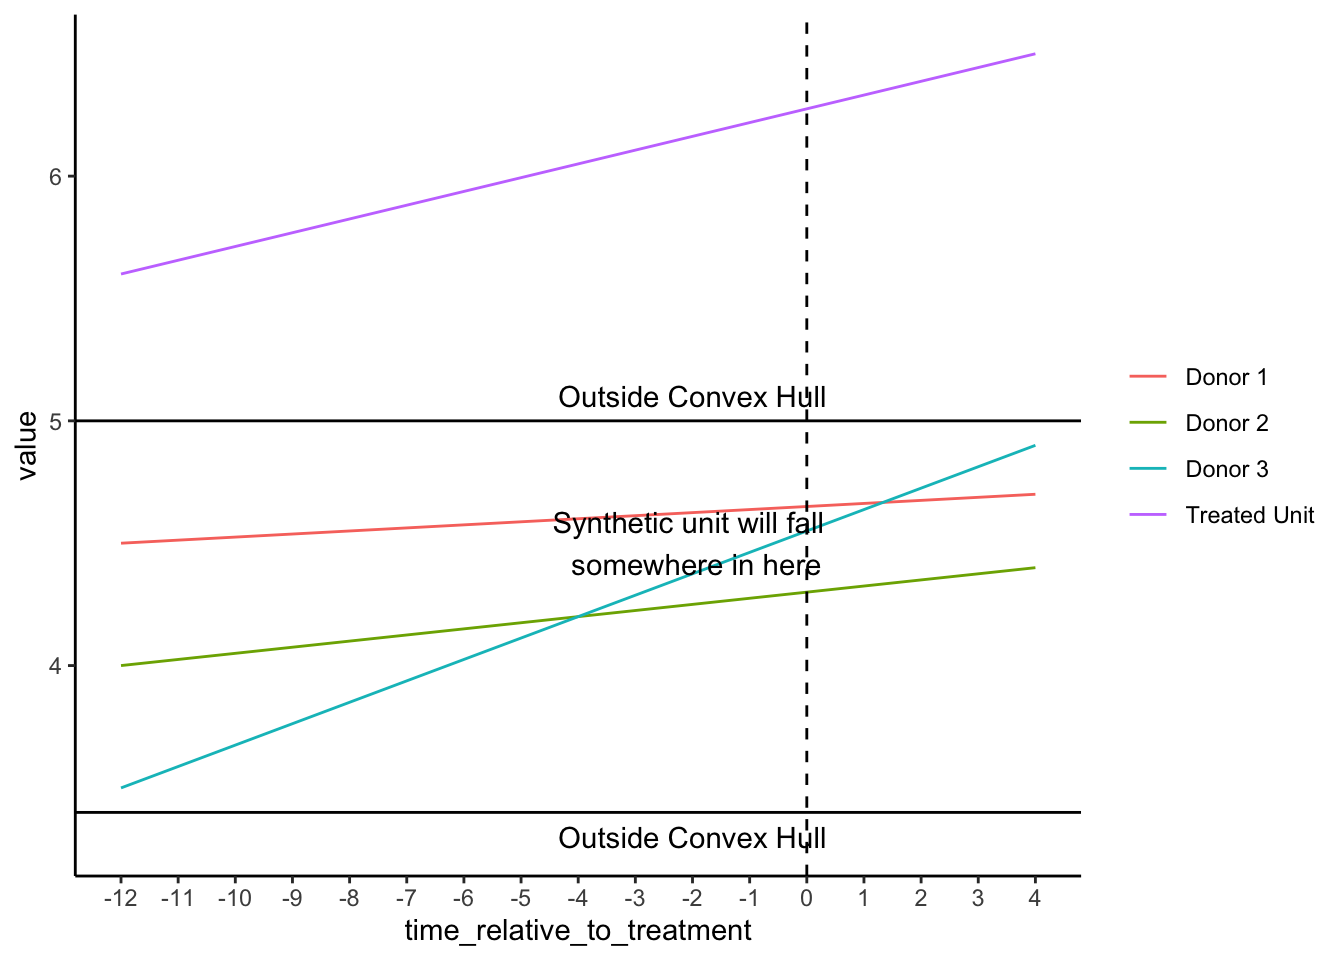
\includegraphics[keepaspectratio]{linear-regression_files/figure-pdf/unnamed-chunk-13-1.pdf}}

So we have it looking at the MSE but we can also look at it with R2

\begin{Shaded}
\begin{Highlighting}[]
\NormalTok{ridge\_cv }\OperatorTok{=}\NormalTok{ ElasticNetCV(alphas }\OperatorTok{=}\NormalTok{ lambdas,}
\NormalTok{                        l1\_ratio }\OperatorTok{=} \DecValTok{0}\NormalTok{,}
\NormalTok{                        cv }\OperatorTok{=}\NormalTok{ kfold)}


\NormalTok{pipe\_cv }\OperatorTok{=}\NormalTok{ Pipeline(steps }\OperatorTok{=}\NormalTok{[(}\StringTok{\textquotesingle{}scaler\textquotesingle{}}\NormalTok{, scaler), (}\StringTok{\textquotesingle{}ridge\textquotesingle{}}\NormalTok{, ridge\_cv)])       }

\NormalTok{pipe\_cv.fit(x, y)}
\end{Highlighting}
\end{Shaded}

\begin{verbatim}
Pipeline(steps=[('scaler', StandardScaler()),
                ('ridge',
                 ElasticNetCV(alphas=array([2.37276310e+05, 1.88037418e+05, 1.49016438e+05, 1.18092979e+05,
       9.35866661e+04, 7.41658324e+04, 5.87751538e+04, 4.65783042e+04,
       3.69125096e+04, 2.92525326e+04, 2.31821318e+04, 1.83714430e+04,
       1.45590544e+04, 1.15378016e+04, 9.14351047e+03, 7.24607567e+03,
       5.74239105e+03, 4.55074670e+03,...
       1.96990961e-03, 1.56111968e-03, 1.23716065e-03, 9.80428657e-04,
       7.76972943e-04, 6.15737770e-04, 4.87961653e-04, 3.86701265e-04,
       3.06454139e-04, 2.42859664e-04, 1.92462131e-04, 1.52522947e-04,
       1.20871827e-04, 9.57888560e-05, 7.59110302e-05, 6.01581933e-05,
       4.76743393e-05, 3.77810986e-05, 2.99408745e-05, 2.37276310e-05]),
                              cv=KFold(n_splits=5, random_state=0, shuffle=True),
                              l1_ratio=0))])
\end{verbatim}

\begin{Shaded}
\begin{Highlighting}[]
\NormalTok{tuned\_ridge }\OperatorTok{=}\NormalTok{ pipe\_cv.named\_steps[}\StringTok{\textquotesingle{}ridge\textquotesingle{}}\NormalTok{]}
\NormalTok{ridgeCV\_fig, ax }\OperatorTok{=}\NormalTok{ plt.subplots(figsize}\OperatorTok{=}\NormalTok{(}\DecValTok{8}\NormalTok{,}\DecValTok{8}\NormalTok{))}
\NormalTok{ax.errorbar(}\OperatorTok{{-}}\NormalTok{np.log(lambdas),}
\NormalTok{            tuned\_ridge.mse\_path\_.mean(}\DecValTok{1}\NormalTok{),}
\NormalTok{            yerr}\OperatorTok{=}\NormalTok{tuned\_ridge.mse\_path\_.std(}\DecValTok{1}\NormalTok{) }\OperatorTok{/}\NormalTok{ np.sqrt(K))}
\NormalTok{ax.axvline(}\OperatorTok{{-}}\NormalTok{np.log(tuned\_ridge.alpha\_), c}\OperatorTok{=}\StringTok{\textquotesingle{}k\textquotesingle{}}\NormalTok{, ls}\OperatorTok{=}\StringTok{\textquotesingle{}{-}{-}\textquotesingle{}}\NormalTok{)}
\NormalTok{ax.set\_ylim([}\DecValTok{50000}\NormalTok{,}\DecValTok{250000}\NormalTok{])}
\end{Highlighting}
\end{Shaded}

\begin{verbatim}
(50000.0, 250000.0)
\end{verbatim}

\begin{Shaded}
\begin{Highlighting}[]
\NormalTok{ax.set\_xlabel(}\StringTok{\textquotesingle{}${-}\textbackslash{}log(\textbackslash{}lambda)$\textquotesingle{}}\NormalTok{, fontsize}\OperatorTok{=}\DecValTok{20}\NormalTok{)}
\NormalTok{ax.set\_ylabel(}\StringTok{\textquotesingle{}Cross{-}validated MSE\textquotesingle{}}\NormalTok{, fontsize}\OperatorTok{=}\DecValTok{20}\NormalTok{)                   }
\end{Highlighting}
\end{Shaded}

\pandocbounded{\includegraphics[keepaspectratio]{linear-regression_files/figure-pdf/unnamed-chunk-14-3.pdf}}

We could do the same thing with a lasso regression but this workflow is
not great instead we can make a function and then loop over the grids.

\begin{Shaded}
\begin{Highlighting}[]

\NormalTok{models }\OperatorTok{=}\NormalTok{ \{}
    \StringTok{\textquotesingle{}ridge\textquotesingle{}}\NormalTok{: ElasticNet(l1\_ratio}\OperatorTok{=}\DecValTok{0}\NormalTok{),}
    \StringTok{\textquotesingle{}lasso\textquotesingle{}}\NormalTok{: ElasticNet(l1\_ratio}\OperatorTok{=}\DecValTok{1}\NormalTok{)  }\CommentTok{\# Lasso is a special case of ElasticNet}
\NormalTok{\}}

\CommentTok{\# Prepare for GridSearchCV}

\NormalTok{param\_grids }\OperatorTok{=}\NormalTok{ \{}
    \StringTok{\textquotesingle{}ridge\textquotesingle{}}\NormalTok{: \{}\StringTok{\textquotesingle{}elasticnet\_\_alpha\textquotesingle{}}\NormalTok{: lambdas\},  }\CommentTok{\# Use \textquotesingle{}elasticnet\textquotesingle{} as the step name}
    \StringTok{\textquotesingle{}lasso\textquotesingle{}}\NormalTok{: \{}\StringTok{\textquotesingle{}elasticnet\_\_alpha\textquotesingle{}}\NormalTok{: lambdas\}}
\NormalTok{\}}

\NormalTok{results }\OperatorTok{=}\NormalTok{ []}
\CommentTok{\# Set up ShuffleSplit cross{-}validation for GridSearchCV}
\NormalTok{validation }\OperatorTok{=}\NormalTok{ ShuffleSplit(n\_splits}\OperatorTok{=}\DecValTok{1}\NormalTok{, test\_size}\OperatorTok{=}\FloatTok{0.5}\NormalTok{, random\_state}\OperatorTok{=}\DecValTok{0}\NormalTok{)}

\CommentTok{\# Function to perform grid search and output results}
\KeywordTok{def}\NormalTok{ tune\_model(model\_name, model, param\_grid):}
    \CommentTok{\# Build pipeline}
\NormalTok{    pipe }\OperatorTok{=}\NormalTok{ Pipeline(steps}\OperatorTok{=}\NormalTok{[(}\StringTok{\textquotesingle{}scaler\textquotesingle{}}\NormalTok{, scaler), (}\StringTok{\textquotesingle{}elasticnet\textquotesingle{}}\NormalTok{, model)])  }\CommentTok{\# Step name matches model\_name}
    
    \CommentTok{\# Perform grid search}
\NormalTok{    grid }\OperatorTok{=}\NormalTok{ GridSearchCV(pipe, param\_grid, cv}\OperatorTok{=}\NormalTok{validation, scoring}\OperatorTok{=}\StringTok{\textquotesingle{}neg\_mean\_squared\_error\textquotesingle{}}\NormalTok{)}
\NormalTok{    grid.fit(x\_train, y\_train)}
    
    \CommentTok{\# Extract best parameters and model}
\NormalTok{    best\_alpha }\OperatorTok{=}\NormalTok{ grid.best\_params\_[}\StringTok{\textquotesingle{}elasticnet\_\_alpha\textquotesingle{}}\NormalTok{]}
\NormalTok{    best\_model }\OperatorTok{=}\NormalTok{ grid.best\_estimator\_}
\NormalTok{    results.append(\{}
        \StringTok{\textquotesingle{}model\textquotesingle{}}\NormalTok{: model\_name.capitalize(),  }\CommentTok{\# Store as "Ridge" or "Lasso"}
        \StringTok{\textquotesingle{}best\_alpha\textquotesingle{}}\NormalTok{: best\_alpha,}
        \StringTok{\textquotesingle{}best\_model\textquotesingle{}}\NormalTok{: }\BuiltInTok{str}\NormalTok{(best\_model),}
        \StringTok{\textquotesingle{}best\_score\textquotesingle{}}\NormalTok{: grid.best\_score\_}
\NormalTok{    \})}
    \ControlFlowTok{return}\NormalTok{ best\_model}
    
\NormalTok{best\_models }\OperatorTok{=}\NormalTok{ \{\}}
\CommentTok{\# Tune each model}
\ControlFlowTok{for}\NormalTok{ model\_name, model }\KeywordTok{in}\NormalTok{ models.items():}
\NormalTok{    best\_models[model\_name] }\OperatorTok{=}\NormalTok{ tune\_model(model\_name, model, param\_grids[model\_name])}


\NormalTok{results\_df }\OperatorTok{=}\NormalTok{ pl.DataFrame(results)}
\end{Highlighting}
\end{Shaded}

So now we have the best model but we would like to grab the most
important features. We may need something to present to stakeholders or
to better understand what is going on in our models.

\begin{Shaded}
\begin{Highlighting}[]
\KeywordTok{def}\NormalTok{ get\_variable\_importance(best\_model, feature\_names):}
    \CommentTok{\# Access the \textquotesingle{}elasticnet\textquotesingle{} step in the pipeline}
\NormalTok{    elastic\_net\_step }\OperatorTok{=}\NormalTok{ best\_model.named\_steps[}\StringTok{\textquotesingle{}elasticnet\textquotesingle{}}\NormalTok{]}
\NormalTok{    coef }\OperatorTok{=}\NormalTok{ elastic\_net\_step.coef\_}
\NormalTok{    feature\_importance }\OperatorTok{=} \BuiltInTok{sorted}\NormalTok{(}\BuiltInTok{zip}\NormalTok{(feature\_names, coef), key}\OperatorTok{=}\KeywordTok{lambda}\NormalTok{ x: }\BuiltInTok{abs}\NormalTok{(x[}\DecValTok{1}\NormalTok{]), reverse}\OperatorTok{=}\VariableTok{True}\NormalTok{)}
\NormalTok{    features, coefficients }\OperatorTok{=} \BuiltInTok{zip}\NormalTok{(}\OperatorTok{*}\NormalTok{feature\_importance)}
    \ControlFlowTok{return}\NormalTok{ features, coefficients}
\CommentTok{\# Prepare side{-}by{-}side plots}
\NormalTok{fig, axes }\OperatorTok{=}\NormalTok{ plt.subplots(}\DecValTok{1}\NormalTok{, }\BuiltInTok{len}\NormalTok{(best\_models), figsize}\OperatorTok{=}\NormalTok{(}\DecValTok{15}\NormalTok{, }\DecValTok{6}\NormalTok{), sharey}\OperatorTok{=}\VariableTok{True}\NormalTok{)}

\CommentTok{\# Get feature names}
\NormalTok{feature\_names }\OperatorTok{=}\NormalTok{ x.columns}

\CommentTok{\# Plot VIP for each model}
\ControlFlowTok{for}\NormalTok{ i, (model\_name, best\_model) }\KeywordTok{in} \BuiltInTok{enumerate}\NormalTok{(best\_models.items()):}
    \CommentTok{\# Extract variable importance}
\NormalTok{    features, coefficients }\OperatorTok{=}\NormalTok{ get\_variable\_importance(best\_model, feature\_names)}
    
    \CommentTok{\# Determine bar colors based on coefficient sign}
\NormalTok{    colors }\OperatorTok{=}\NormalTok{ [}\StringTok{\textquotesingle{}green\textquotesingle{}} \ControlFlowTok{if}\NormalTok{ coef }\OperatorTok{\textgreater{}} \DecValTok{0} \ControlFlowTok{else} \StringTok{\textquotesingle{}red\textquotesingle{}} \ControlFlowTok{for}\NormalTok{ coef }\KeywordTok{in}\NormalTok{ coefficients]}
    
    \CommentTok{\# Create subplot}
\NormalTok{    axes[i].barh(features, np.}\BuiltInTok{abs}\NormalTok{(coefficients), color}\OperatorTok{=}\NormalTok{colors)}
\NormalTok{    axes[i].set\_title(}\SpecialStringTok{f\textquotesingle{}Variable Importance: }\SpecialCharTok{\{}\NormalTok{model\_name}\SpecialCharTok{.}\NormalTok{capitalize()}\SpecialCharTok{\}}\SpecialStringTok{\textquotesingle{}}\NormalTok{)}
\NormalTok{    axes[i].set\_xlabel(}\StringTok{\textquotesingle{}Absolute Coefficient Value\textquotesingle{}}\NormalTok{)}
    \ControlFlowTok{if}\NormalTok{ i }\OperatorTok{==} \DecValTok{0}\NormalTok{:  }\CommentTok{\# Add y{-}axis label only for the first plot}
\NormalTok{        axes[i].set\_ylabel(}\StringTok{\textquotesingle{}Features\textquotesingle{}}\NormalTok{)}
\NormalTok{    axes[i].invert\_yaxis()  }\CommentTok{\# Invert y{-}axis for descending order}
    
    \CommentTok{\# Add a legend}
\NormalTok{    axes[i].legend([}\StringTok{\textquotesingle{}Positive Impact\textquotesingle{}}\NormalTok{, }\StringTok{\textquotesingle{}Negative Impact\textquotesingle{}}\NormalTok{], loc}\OperatorTok{=}\StringTok{\textquotesingle{}lower right\textquotesingle{}}\NormalTok{)}

\CommentTok{\# Adjust layout}
\NormalTok{plt.tight\_layout()}
\NormalTok{plt.show()}
\end{Highlighting}
\end{Shaded}

\pandocbounded{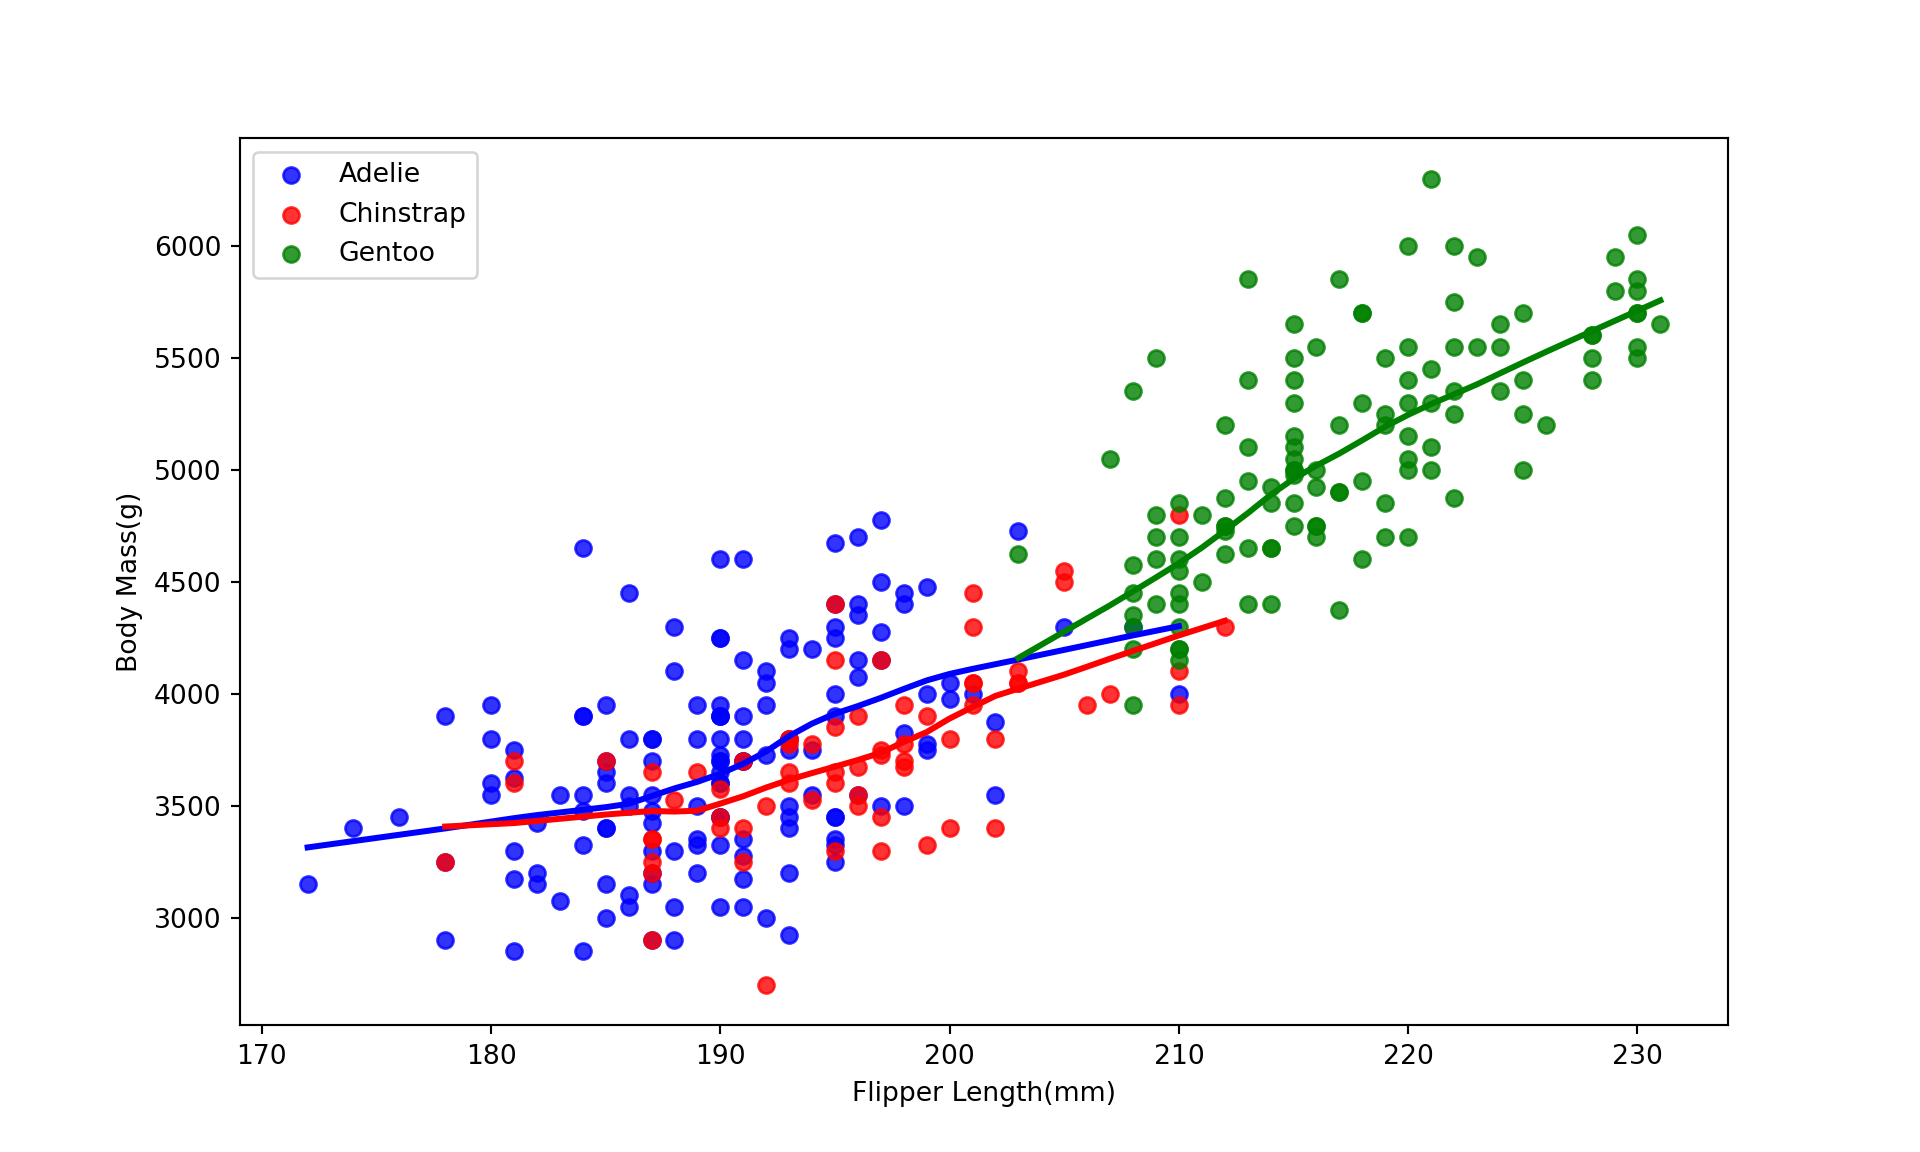
\includegraphics[keepaspectratio]{linear-regression_files/figure-pdf/unnamed-chunk-16-5.pdf}}

Which is nice we see what is postively impacting value. However, I don't
neccessarily like these plots since we are not really showing anything
interesting. A better way would be to show marginal effects. However
right now we are kind of lacking that on the python side. In R this is
somewhat trivial but

\begin{Shaded}
\begin{Highlighting}[]
\FunctionTok{library}\NormalTok{(tidymodels)}
\FunctionTok{library}\NormalTok{(marginaleffects)}
\FunctionTok{library}\NormalTok{(ISLR)}

\NormalTok{Hitters }\OtherTok{\textless{}{-}} \FunctionTok{as\_tibble}\NormalTok{(Hitters) }\SpecialCharTok{\%\textgreater{}\%}
  \FunctionTok{filter}\NormalTok{(}\SpecialCharTok{!}\FunctionTok{is.na}\NormalTok{(Salary))}

\NormalTok{Hitters\_split }\OtherTok{\textless{}{-}} \FunctionTok{initial\_split}\NormalTok{(Hitters, }\AttributeTok{strata =} \StringTok{"Salary"}\NormalTok{)}

\NormalTok{Hitters\_train }\OtherTok{\textless{}{-}} \FunctionTok{training}\NormalTok{(Hitters\_split)}
\NormalTok{Hitters\_test }\OtherTok{\textless{}{-}} \FunctionTok{testing}\NormalTok{(Hitters\_split)}

\NormalTok{Hitters\_fold }\OtherTok{\textless{}{-}} \FunctionTok{vfold\_cv}\NormalTok{(Hitters\_train, }\AttributeTok{v =} \DecValTok{10}\NormalTok{)}


\NormalTok{ridge\_recipe }\OtherTok{\textless{}{-}} 
  \FunctionTok{recipe}\NormalTok{(}\AttributeTok{formula =}\NormalTok{ Salary }\SpecialCharTok{\textasciitilde{}}\NormalTok{ ., }\AttributeTok{data =}\NormalTok{ Hitters\_train) }\SpecialCharTok{\%\textgreater{}\%} 
  \FunctionTok{step\_novel}\NormalTok{(}\FunctionTok{all\_nominal\_predictors}\NormalTok{()) }\SpecialCharTok{\%\textgreater{}\%} 
  \FunctionTok{step\_dummy}\NormalTok{(}\FunctionTok{all\_nominal\_predictors}\NormalTok{()) }\SpecialCharTok{\%\textgreater{}\%} 
  \FunctionTok{step\_zv}\NormalTok{(}\FunctionTok{all\_predictors}\NormalTok{()) }\SpecialCharTok{\%\textgreater{}\%} 
  \FunctionTok{step\_normalize}\NormalTok{(}\FunctionTok{all\_predictors}\NormalTok{())}

\NormalTok{ridge\_spec }\OtherTok{\textless{}{-}} 
  \FunctionTok{linear\_reg}\NormalTok{(}\AttributeTok{penalty =} \FunctionTok{tune}\NormalTok{(), }\AttributeTok{mixture =} \DecValTok{0}\NormalTok{) }\SpecialCharTok{\%\textgreater{}\%} 
  \FunctionTok{set\_mode}\NormalTok{(}\StringTok{"regression"}\NormalTok{) }\SpecialCharTok{\%\textgreater{}\%} 
  \FunctionTok{set\_engine}\NormalTok{(}\StringTok{"glmnet"}\NormalTok{)}

\NormalTok{ridge\_workflow }\OtherTok{\textless{}{-}} \FunctionTok{workflow}\NormalTok{() }\SpecialCharTok{\%\textgreater{}\%} 
  \FunctionTok{add\_recipe}\NormalTok{(ridge\_recipe) }\SpecialCharTok{\%\textgreater{}\%} 
  \FunctionTok{add\_model}\NormalTok{(ridge\_spec)}

\NormalTok{penalty\_grid }\OtherTok{\textless{}{-}} \FunctionTok{grid\_regular}\NormalTok{(}\FunctionTok{penalty}\NormalTok{(}\AttributeTok{range =} \FunctionTok{c}\NormalTok{(}\SpecialCharTok{{-}}\DecValTok{5}\NormalTok{, }\DecValTok{5}\NormalTok{)), }\AttributeTok{levels =} \DecValTok{50}\NormalTok{)}

\NormalTok{tune\_res }\OtherTok{\textless{}{-}} \FunctionTok{tune\_grid}\NormalTok{(}
\NormalTok{  ridge\_workflow,}
  \AttributeTok{resamples =}\NormalTok{ Hitters\_fold, }
  \AttributeTok{grid =}\NormalTok{ penalty\_grid}
\NormalTok{)}

\NormalTok{best\_penalty }\OtherTok{=} \FunctionTok{select\_best}\NormalTok{(tune\_res, }\AttributeTok{metric =} \StringTok{\textquotesingle{}rsq\textquotesingle{}}\NormalTok{)}

\NormalTok{ridge\_final }\OtherTok{\textless{}{-}} \FunctionTok{finalize\_workflow}\NormalTok{(ridge\_workflow, best\_penalty)}

\NormalTok{ridge\_final\_fit }\OtherTok{\textless{}{-}} \FunctionTok{fit}\NormalTok{(ridge\_final, }\AttributeTok{data =}\NormalTok{ Hitters\_train)}

\FunctionTok{avg\_predictions}\NormalTok{(ridge\_final\_fit, }\AttributeTok{newdata =}\NormalTok{ Hitters\_test)}
\end{Highlighting}
\end{Shaded}

\bookmarksetup{startatroot}

\chapter{Classification}\label{classification}

\begin{Shaded}
\begin{Highlighting}[]
\ImportTok{from}\NormalTok{ sklearn.linear\_model }\ImportTok{import}\NormalTok{ LogisticRegression}
\ImportTok{from}\NormalTok{ sklearn.discriminant\_analysis }\ImportTok{import}\NormalTok{ LinearDiscriminantAnalysis}
\ImportTok{from}\NormalTok{ sklearn.naive\_bayes }\ImportTok{import}\NormalTok{ GaussianNB}
\ImportTok{from}\NormalTok{ sklearn.neighbors }\ImportTok{import}\NormalTok{ KNeighborsClassifier}
\ImportTok{from}\NormalTok{ sklearn.model\_selection }\ImportTok{import}\NormalTok{ train\_test\_split}
\ImportTok{from}\NormalTok{ sklearn.model\_selection }\ImportTok{import}\NormalTok{ cross\_val\_score}
\ImportTok{import}\NormalTok{ xgboost }\ImportTok{as}\NormalTok{ xgb}
\ImportTok{from}\NormalTok{ sklearn.inspection }\ImportTok{import}\NormalTok{ PartialDependenceDisplay}
\ImportTok{from}\NormalTok{ sklearn.metrics }\ImportTok{import}\NormalTok{ accuracy\_score, precision\_score, recall\_score, f1\_score, roc\_auc\_score, confusion\_matrix, classification\_report, ConfusionMatrixDisplay}
\ImportTok{import}\NormalTok{ statsmodels.api }\ImportTok{as}\NormalTok{ sm}
\ImportTok{import}\NormalTok{ statsmodels.formula.api }\ImportTok{as}\NormalTok{ smf}
\ImportTok{import}\NormalTok{ numpy }\ImportTok{as}\NormalTok{ np}
\ImportTok{import}\NormalTok{ matplotlib.pyplot }\ImportTok{as}\NormalTok{ plt}
\ImportTok{import}\NormalTok{ polars }\ImportTok{as}\NormalTok{ pl }
\ImportTok{import}\NormalTok{ polars.selectors }\ImportTok{as}\NormalTok{ cs }
\ImportTok{from}\NormalTok{ sklearn.datasets }\ImportTok{import}\NormalTok{ make\_classification}

\NormalTok{stocks }\OperatorTok{=}\NormalTok{ pl.read\_csv(}\StringTok{\textquotesingle{}data/Smarket.csv\textquotesingle{}}\NormalTok{)}
\end{Highlighting}
\end{Shaded}

Lets work through a somewhat contrived example. Lets say we wanted to
predict the whether the stock market is going up or down. This is not
neccessarily all that interesting but will be good practice. Lets
visualize the data

\begin{Shaded}
\begin{Highlighting}[]
\NormalTok{corrs }\OperatorTok{=}\NormalTok{ stocks.select(}\OperatorTok{\textasciitilde{}}\NormalTok{cs.string()).corr()}

\NormalTok{corrs }
\end{Highlighting}
\end{Shaded}

\begin{verbatim}
shape: (8, 8)
┌──────────┬───────────┬───────────┬───────────┬───────────┬───────────┬───────────┬───────────┐
│ Year     ┆ Lag1      ┆ Lag2      ┆ Lag3      ┆ Lag4      ┆ Lag5      ┆ Volume    ┆ Today     │
│ ---      ┆ ---       ┆ ---       ┆ ---       ┆ ---       ┆ ---       ┆ ---       ┆ ---       │
│ f64      ┆ f64       ┆ f64       ┆ f64       ┆ f64       ┆ f64       ┆ f64       ┆ f64       │
╞══════════╪═══════════╪═══════════╪═══════════╪═══════════╪═══════════╪═══════════╪═══════════╡
│ 1.0      ┆ 0.0297    ┆ 0.030596  ┆ 0.033195  ┆ 0.035689  ┆ 0.029788  ┆ 0.539006  ┆ 0.030095  │
│ 0.0297   ┆ 1.0       ┆ -0.026294 ┆ -0.010803 ┆ -0.002986 ┆ -0.005675 ┆ 0.04091   ┆ -0.026155 │
│ 0.030596 ┆ -0.026294 ┆ 1.0       ┆ -0.025897 ┆ -0.010854 ┆ -0.003558 ┆ -0.043383 ┆ -0.01025  │
│ 0.033195 ┆ -0.010803 ┆ -0.025897 ┆ 1.0       ┆ -0.024051 ┆ -0.018808 ┆ -0.041824 ┆ -0.002448 │
│ 0.035689 ┆ -0.002986 ┆ -0.010854 ┆ -0.024051 ┆ 1.0       ┆ -0.027084 ┆ -0.048414 ┆ -0.0069   │
│ 0.029788 ┆ -0.005675 ┆ -0.003558 ┆ -0.018808 ┆ -0.027084 ┆ 1.0       ┆ -0.022002 ┆ -0.03486  │
│ 0.539006 ┆ 0.04091   ┆ -0.043383 ┆ -0.041824 ┆ -0.048414 ┆ -0.022002 ┆ 1.0       ┆ 0.014592  │
│ 0.030095 ┆ -0.026155 ┆ -0.01025  ┆ -0.002448 ┆ -0.0069   ┆ -0.03486  ┆ 0.014592  ┆ 1.0       │
└──────────┴───────────┴───────────┴───────────┴───────────┴───────────┴───────────┴───────────┘
\end{verbatim}

We may also want to see some descriptives. A line plot would be nice but
it would kind of hide alot so we are going to make a beeswarm plot

\begin{Shaded}
\begin{Highlighting}[]
\NormalTok{years\_unique }\OperatorTok{=}\NormalTok{ stocks.unique(subset}\OperatorTok{=}\StringTok{"Year"}\NormalTok{)[}\StringTok{"Year"}\NormalTok{].to\_list()}

\NormalTok{years\_num }\OperatorTok{=}\NormalTok{ \{year: i }\ControlFlowTok{for}\NormalTok{ i, year }\KeywordTok{in} \BuiltInTok{enumerate}\NormalTok{(years\_unique)\}}

\ControlFlowTok{for}\NormalTok{ years }\KeywordTok{in}\NormalTok{ years\_unique:}
\NormalTok{    year\_data }\OperatorTok{=}\NormalTok{ stocks.}\BuiltInTok{filter}\NormalTok{(pl.col(}\StringTok{"Year"}\NormalTok{) }\OperatorTok{==}\NormalTok{ years)}
\NormalTok{    y }\OperatorTok{=}\NormalTok{ year\_data[}\StringTok{"Volume"}\NormalTok{].to\_numpy()}
\NormalTok{    x }\OperatorTok{=}\NormalTok{ np.random.normal(years\_num[years], }\FloatTok{0.1}\NormalTok{, }\BuiltInTok{len}\NormalTok{(y))}

\NormalTok{    plt.scatter(x, y)}


\NormalTok{plt.xticks(}\BuiltInTok{range}\NormalTok{(}\BuiltInTok{len}\NormalTok{(years\_unique)), }\BuiltInTok{sorted}\NormalTok{(years\_unique))}
\end{Highlighting}
\end{Shaded}

\begin{verbatim}
([<matplotlib.axis.XTick object at 0x357039150>, <matplotlib.axis.XTick object at 0x357b02310>, <matplotlib.axis.XTick object at 0x356603210>, <matplotlib.axis.XTick object at 0x357b41890>, <matplotlib.axis.XTick object at 0x357b43d50>], [Text(0, 0, '2001'), Text(1, 0, '2002'), Text(2, 0, '2003'), Text(3, 0, '2004'), Text(4, 0, '2005')])
\end{verbatim}

\begin{Shaded}
\begin{Highlighting}[]
\NormalTok{plt.ylabel(}\StringTok{"Trading Volume"}\NormalTok{)}
\NormalTok{plt.xlabel(}\StringTok{"Year"}\NormalTok{)}
\end{Highlighting}
\end{Shaded}

\pandocbounded{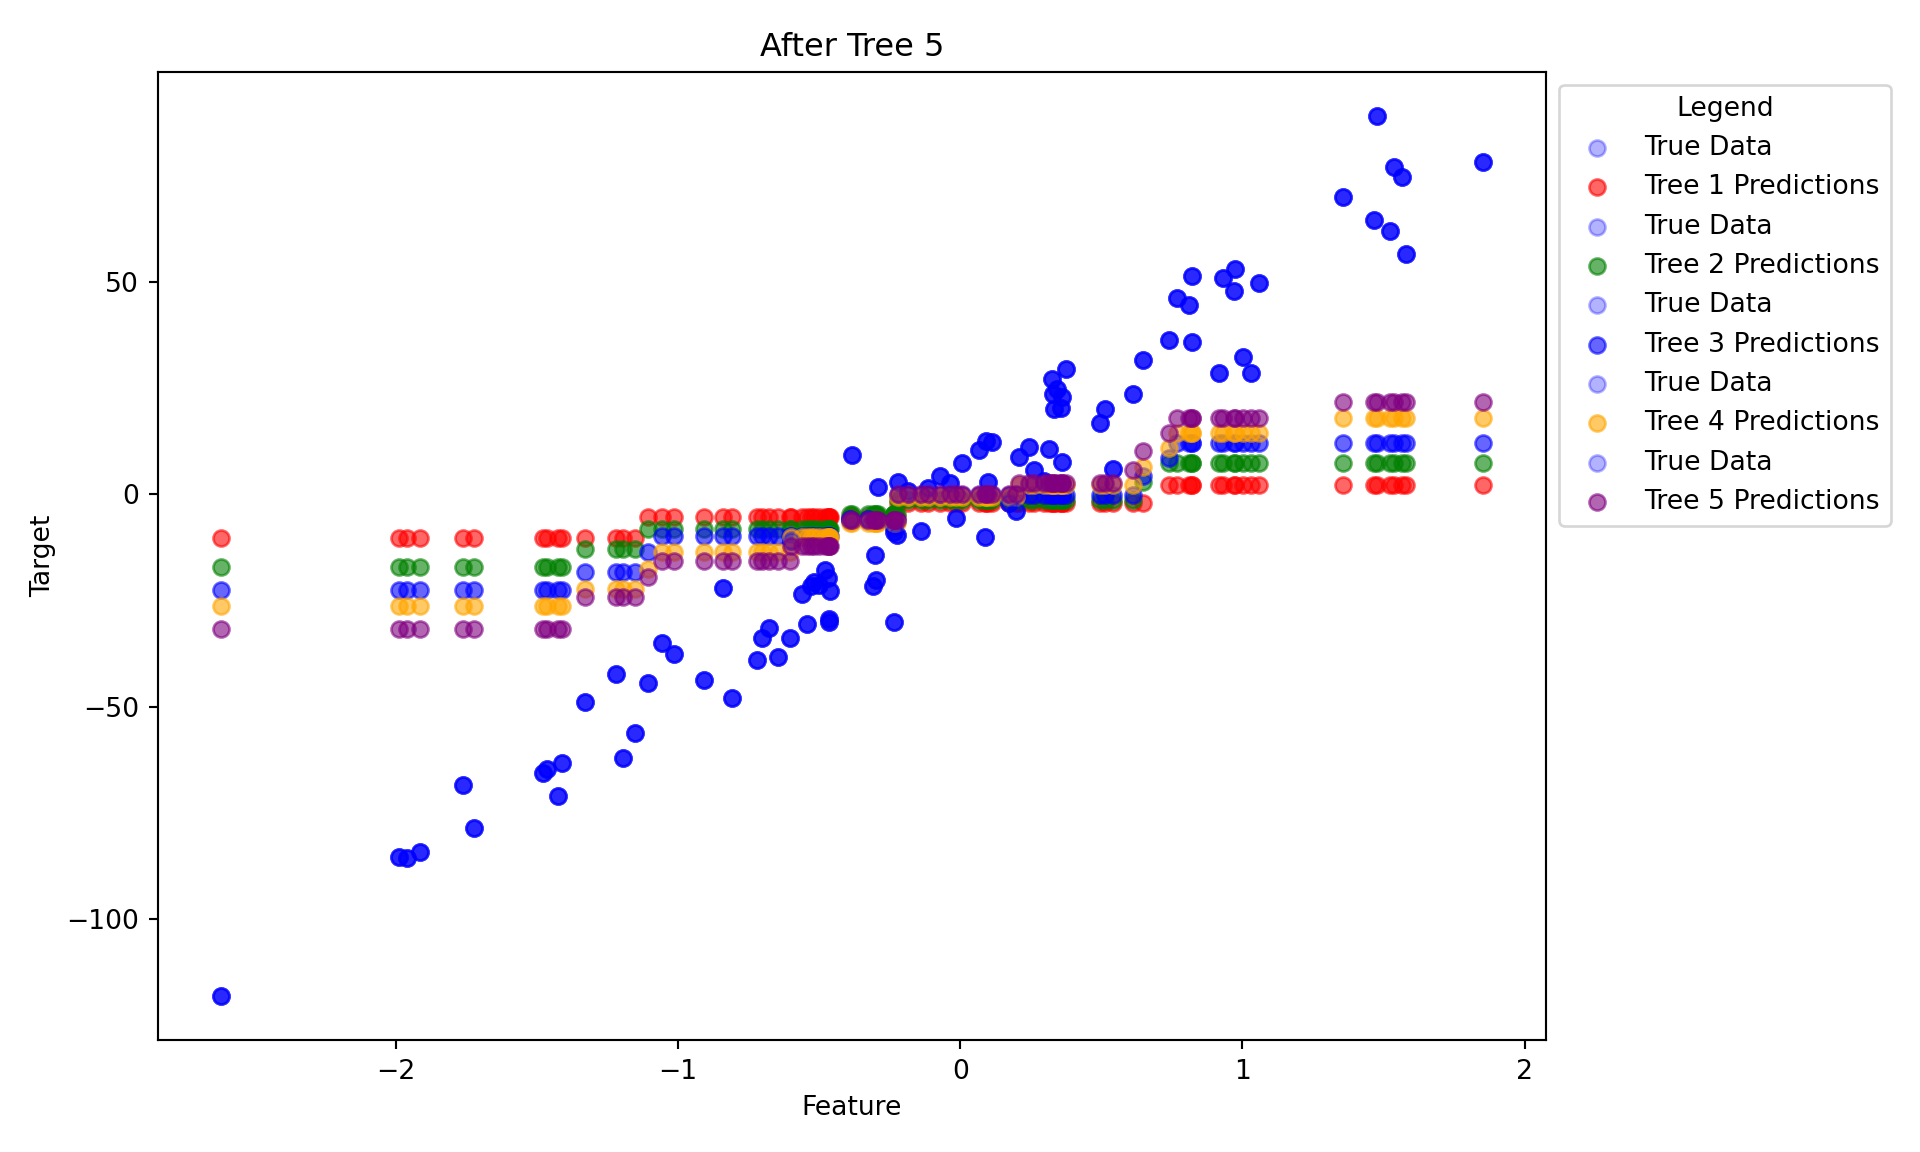
\includegraphics[keepaspectratio]{classification_files/figure-pdf/unnamed-chunk-3-1.pdf}}

We are slowly but surely seeing an upwardsish trend in trading volume.
There are definitely more graphs that we can make but for now we are
going to move to the study portion.

\section{Logistic Regression}\label{logistic-regression}

Logistic regression is probably your first classifier and is an
incredibly important. They are a subfamily of Maximum Likelihood
estimation. In a canned example lets say we have the a coin flip and we
do it like a ton of times. We record each outcome where the probability
is defined something like this.

\begin{align}
P(Heads) = \frac{number of heads}{number of tosses} \\
P(Tails) = 1 - P(Heads)
 

\end{align}

We have some data and now we want to model it. We take the joint
probablility as the function of some parameters aka the likelihood
function. The value of theta that maxmimizes the likelihood function is
called the maximum likelihood estimator.

Logit is just a sub estimator of these estimators where we make the
assumption that the DGP follows a binomial distribution and that the
most appropriate link function is the logistic link which is just a
technical sounding way of saying we are taking the log of
\(\frac{p}{1-p}\). This is really usefull because we bound the odds of
an event happening between 0-1. The problem with MLE is that when
underneath the hood we are logging the likelihood function because well
prior to the invention of computer with this much power you would never
be able to hand derive these things, but we still had data to model.

\subsection{Modeling it in Python}\label{modeling-it-in-python}

Lets take our stock market data and try to classify whether the
direction is up or down using contemporaneous volumne and what appears
to be lags of volume. Using the Stats model api we can do it like this

\begin{Shaded}
\begin{Highlighting}[]
\NormalTok{stocks\_pd }\OperatorTok{=}\NormalTok{ stocks.with\_columns(}
\NormalTok{    direction }\OperatorTok{=}\NormalTok{ pl.when(pl.col(}\StringTok{\textquotesingle{}Direction\textquotesingle{}}\NormalTok{) }\OperatorTok{==} \StringTok{\textquotesingle{}Up\textquotesingle{}}\NormalTok{).then(}\DecValTok{1}\NormalTok{).otherwise(}\DecValTok{0}\NormalTok{)}
\NormalTok{)}

\NormalTok{form\_version }\OperatorTok{=}\NormalTok{ smf.logit(}\StringTok{\textquotesingle{}direction \textasciitilde{} Lag1 + Lag2 + Lag3 + Lag4 + Lag5 + Volume\textquotesingle{}}\NormalTok{, data }\OperatorTok{=}\NormalTok{ stocks\_pd.to\_pandas()).fit()}
\end{Highlighting}
\end{Shaded}

\begin{verbatim}
Optimization terminated successfully.
         Current function value: 0.691034
         Iterations 4
\end{verbatim}

\begin{Shaded}
\begin{Highlighting}[]
\NormalTok{x }\OperatorTok{=}\NormalTok{ stocks\_pd.drop([}\StringTok{\textquotesingle{}Direction\textquotesingle{}}\NormalTok{, }\StringTok{\textquotesingle{}direction\textquotesingle{}}\NormalTok{, }\StringTok{\textquotesingle{}Year\textquotesingle{}}\NormalTok{, }\StringTok{\textquotesingle{}Today\textquotesingle{}}\NormalTok{]).to\_numpy()}

\NormalTok{x }\OperatorTok{=}\NormalTok{ sm.add\_constant(x)}

\NormalTok{y }\OperatorTok{=}\NormalTok{ stocks\_pd[}\StringTok{\textquotesingle{}direction\textquotesingle{}}\NormalTok{].to\_numpy()}

\NormalTok{stats\_version }\OperatorTok{=}\NormalTok{ sm.GLM(y, x, family }\OperatorTok{=}\NormalTok{ sm.families.Binomial()).fit()}

\NormalTok{stats\_version.summary()}
\end{Highlighting}
\end{Shaded}

\begin{verbatim}
<class 'statsmodels.iolib.summary.Summary'>
"""
                 Generalized Linear Model Regression Results                  
==============================================================================
Dep. Variable:                      y   No. Observations:                 1250
Model:                            GLM   Df Residuals:                     1243
Model Family:                Binomial   Df Model:                            6
Link Function:                  Logit   Scale:                          1.0000
Method:                          IRLS   Log-Likelihood:                -863.79
Date:                Tue, 04 Feb 2025   Deviance:                       1727.6
Time:                        09:06:09   Pearson chi2:                 1.25e+03
No. Iterations:                     4   Pseudo R-squ. (CS):           0.002868
Covariance Type:            nonrobust                                         
==============================================================================
                 coef    std err          z      P>|z|      [0.025      0.975]
------------------------------------------------------------------------------
const         -0.1260      0.241     -0.523      0.601      -0.598       0.346
x1            -0.0731      0.050     -1.457      0.145      -0.171       0.025
x2            -0.0423      0.050     -0.845      0.398      -0.140       0.056
x3             0.0111      0.050      0.222      0.824      -0.087       0.109
x4             0.0094      0.050      0.187      0.851      -0.089       0.107
x5             0.0103      0.050      0.208      0.835      -0.087       0.107
x6             0.1354      0.158      0.855      0.392      -0.175       0.446
==============================================================================
"""
\end{verbatim}

\begin{Shaded}
\begin{Highlighting}[]
\NormalTok{form\_version.summary()}
\end{Highlighting}
\end{Shaded}

\begin{verbatim}
<class 'statsmodels.iolib.summary.Summary'>
"""
                           Logit Regression Results                           
==============================================================================
Dep. Variable:              direction   No. Observations:                 1250
Model:                          Logit   Df Residuals:                     1243
Method:                           MLE   Df Model:                            6
Date:                Tue, 04 Feb 2025   Pseudo R-squ.:                0.002074
Time:                        09:06:09   Log-Likelihood:                -863.79
converged:                       True   LL-Null:                       -865.59
Covariance Type:            nonrobust   LLR p-value:                    0.7319
==============================================================================
                 coef    std err          z      P>|z|      [0.025      0.975]
------------------------------------------------------------------------------
Intercept     -0.1260      0.241     -0.523      0.601      -0.598       0.346
Lag1          -0.0731      0.050     -1.457      0.145      -0.171       0.025
Lag2          -0.0423      0.050     -0.845      0.398      -0.140       0.056
Lag3           0.0111      0.050      0.222      0.824      -0.087       0.109
Lag4           0.0094      0.050      0.187      0.851      -0.089       0.107
Lag5           0.0103      0.050      0.208      0.835      -0.087       0.107
Volume         0.1354      0.158      0.855      0.392      -0.175       0.446
==============================================================================
"""
\end{verbatim}

To assess our classifier we should go through several steps first we can
look at the confusion matrix. Basically we can get as very general look
at how well our predictions lineup with the actual data. First we need
to get our predictions and then bin them into 1's and zero

\begin{Shaded}
\begin{Highlighting}[]
\NormalTok{form\_preds }\OperatorTok{=}\NormalTok{ form\_version.predict(stocks\_pd.to\_pandas())}

\NormalTok{y\_pred }\OperatorTok{=}\NormalTok{ (form\_preds }\OperatorTok{\textgreater{}=} \FloatTok{0.5}\NormalTok{).astype(}\BuiltInTok{int}\NormalTok{)}

\NormalTok{y\_actual }\OperatorTok{=}\NormalTok{ stocks\_pd[}\StringTok{\textquotesingle{}direction\textquotesingle{}}\NormalTok{].to\_pandas()}

\NormalTok{conf\_mat }\OperatorTok{=}\NormalTok{ confusion\_matrix(y\_actual, y\_pred)}

\NormalTok{disp }\OperatorTok{=}\NormalTok{ ConfusionMatrixDisplay(confusion\_matrix}\OperatorTok{=}\NormalTok{conf\_mat)}

\NormalTok{disp.plot()}
\end{Highlighting}
\end{Shaded}

\begin{verbatim}
<sklearn.metrics._plot.confusion_matrix.ConfusionMatrixDisplay object at 0x36c3ea650>
\end{verbatim}

\pandocbounded{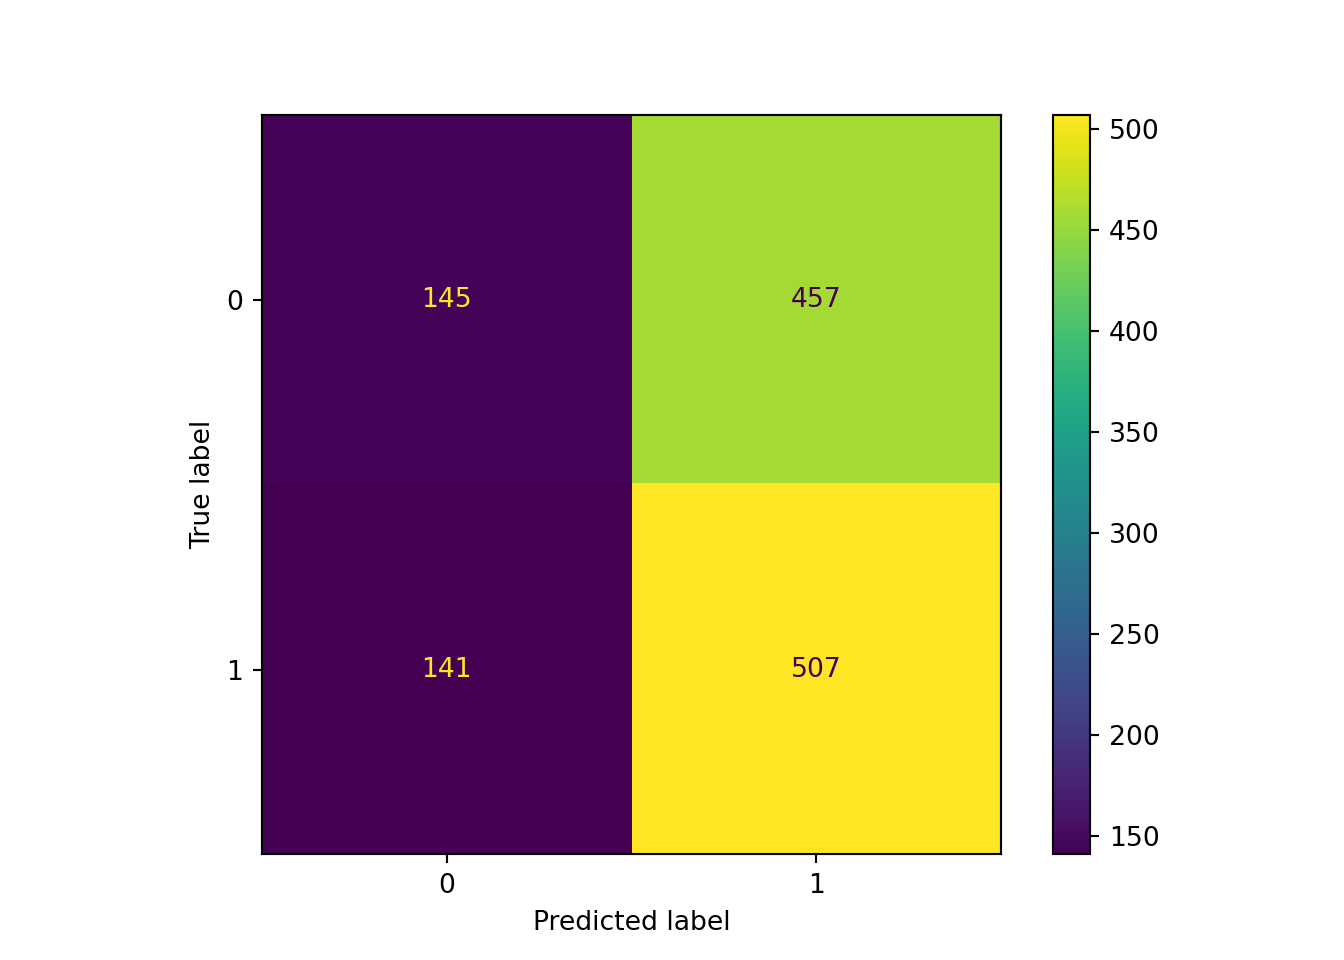
\includegraphics[keepaspectratio]{classification_files/figure-pdf/unnamed-chunk-5-3.pdf}}

This is a nice intuitive display. We are seeing what the model predicted
versus what actually happens. When it comes to classification we have a
variety of metrics.

\begin{align}
\text{Accuracy} = \frac{\text{True Postive} + \text{True Negative}}{TP + TN + FN + FP} \\
\text{Precision} = \frac{TP}{TP + FP} \\
\text{Recall} = \frac{TP}{TP + FN} \\
\text{F1 Score} = 2 \times \frac{precision \times recall}{precision + recall}

\end{align}

Each of these metrics have a variety of benefits and tradeoffs.

\begin{itemize}
\tightlist
\item
  Accuracy
\end{itemize}

Accuracy is nice and intuitive what proportion of correct predictions
are we making? In a perfect world this is the only thing that we would
use when evaluating models. However, if we have a lot of positives and
very few negatives or vice versa our model is going to get good at
predicting positives. But not that great at predicting negatives. When
the class balance is bad enough we are going to get high accuracy
because it is good at predicting the dominant class.

\begin{itemize}
\tightlist
\item
  Precision and Recall
\end{itemize}

Precision is useful if we decompose what is in the denominator. If false
positives are costly meaning that if flagging something as a positive
would lead to not great outcomes we may need to maximize precision.
However, we should always consider how it does with recall. Recall is
the compliment to precision. In this case we are looking at the
proportion of true positives and false negatives.

If we take the case of fraud and think about it like along these lines
we want to strike a balance between the two maybe slightly favoring
recall. While false positives are something we want to mininmize because
it can cause frustrations and eat up company resources. Which isn't good
but significantly more costly. We don't want to miss actual cases of
fraud.

\begin{itemize}
\tightlist
\item
  F1 Score
\end{itemize}

F1 score tries to strike this balance because maximizing precision or
recall will lead the model to overcorrect. F1 score does a bit better
with imbalanced datasets than accuracy the big drawback is we lose the
interpretibility of whether the model is doing better minimizing false
negatives or false positives.

\section{Test Questions}\label{test-questions}

Some times employers will test you on things that aren't just going
through these. One real example you ran into is that you needed to hand
calculate the True postives and the True negatives which you failed
miserably and wasn't able to even get to the rest.

You are working on a classification problem with two classes: Class 1
and Class 2. There are a total of 2000 observations in the dataset, with
1200 observations in Class 1 and 800 observations in Class 2. Your
classifier produces the following predictions:

It assigns 1000 observations to Class 1. It assigns 800 observations to
Class 2. Additionally, your classifier correctly classifies 1000
observations in total.

Using this information:

How many observations are true positives for Class 1 and Class 2? How
many observations are false positives for each class?

For the True Postives we would do some

\begin{Shaded}
\begin{Highlighting}[]
\CommentTok{\# Define the known values}
\NormalTok{correctly\_classified }\OtherTok{\textless{}{-}} \DecValTok{1000}
\NormalTok{predicted\_class1 }\OtherTok{\textless{}{-}} \DecValTok{1000}
\NormalTok{predicted\_class2 }\OtherTok{\textless{}{-}} \DecValTok{800}
\NormalTok{actual\_class1 }\OtherTok{\textless{}{-}} \DecValTok{1200}
\NormalTok{actual\_class2 }\OtherTok{\textless{}{-}} \DecValTok{800}


\NormalTok{TP2 }\OtherTok{\textless{}{-}}\NormalTok{ (predicted\_class2 }\SpecialCharTok{{-}}\NormalTok{ actual\_class1 }\SpecialCharTok{+}\NormalTok{ correctly\_classified) }\SpecialCharTok{/} \DecValTok{2}

\CommentTok{\# Solve for TP1 using TP1 + TP2 = correctly\_classified}
\NormalTok{TP1 }\OtherTok{\textless{}{-}}\NormalTok{ correctly\_classified }\SpecialCharTok{{-}}\NormalTok{ TP2}

\CommentTok{\# Solve for FP1 and FP2}
\NormalTok{FP1 }\OtherTok{\textless{}{-}}\NormalTok{ predicted\_class1 }\SpecialCharTok{{-}}\NormalTok{ TP1}
\NormalTok{FP2 }\OtherTok{\textless{}{-}}\NormalTok{ predicted\_class2 }\SpecialCharTok{{-}}\NormalTok{ TP2}

\NormalTok{TP1 }\SpecialCharTok{+}\NormalTok{ TP2}
\end{Highlighting}
\end{Shaded}

\begin{verbatim}
[1] 1000
\end{verbatim}

\begin{Shaded}
\begin{Highlighting}[]
\CommentTok{\# Print the results}
\FunctionTok{cat}\NormalTok{(}\StringTok{"True Positives for Class 1 (TP1):"}\NormalTok{, TP1, }\StringTok{"}\SpecialCharTok{\textbackslash{}n}\StringTok{"}\NormalTok{)}
\end{Highlighting}
\end{Shaded}

\begin{verbatim}
True Positives for Class 1 (TP1): 700 
\end{verbatim}

\begin{Shaded}
\begin{Highlighting}[]
\FunctionTok{cat}\NormalTok{(}\StringTok{"True Positives for Class 2 (TP2):"}\NormalTok{, TP2, }\StringTok{"}\SpecialCharTok{\textbackslash{}n}\StringTok{"}\NormalTok{)}
\end{Highlighting}
\end{Shaded}

\begin{verbatim}
True Positives for Class 2 (TP2): 300 
\end{verbatim}

\begin{Shaded}
\begin{Highlighting}[]
\FunctionTok{cat}\NormalTok{(}\StringTok{"False Positives for Class 1 (FP1):"}\NormalTok{, FP1, }\StringTok{"}\SpecialCharTok{\textbackslash{}n}\StringTok{"}\NormalTok{)}
\end{Highlighting}
\end{Shaded}

\begin{verbatim}
False Positives for Class 1 (FP1): 300 
\end{verbatim}

\begin{Shaded}
\begin{Highlighting}[]
\FunctionTok{cat}\NormalTok{(}\StringTok{"False Positives for Class 2 (FP2):"}\NormalTok{, FP2, }\StringTok{"}\SpecialCharTok{\textbackslash{}n}\StringTok{"}\NormalTok{)}
\end{Highlighting}
\end{Shaded}

\begin{verbatim}
False Positives for Class 2 (FP2): 500 
\end{verbatim}

\section{Bias Variance Tradeoff}\label{bias-variance-tradeoff}

Right now, our model is good at classifying the data we have. However,
when we introduce new data, it might struggle to generalize and classify
new observations accurately. This challenge arises from overfitting,
where the model is really good at describing the dataset it has already
seen. To mitigate this we split our data into training sets, test sets,
and validation sets effectively hiding parts of our data from our model.
It never has access to every single part of the data. By reducing the
amount of data the model sees it can't learn every single strange data
point in the model.

The reason we do this is because we want our model to predict new data
but also do a good job of approximating the data generating process.
These two goals are inherently conflictual. Bias represents how far away
we are from the target while variance represents how far away our
guesses are from each other. If we build a model that is good at
predicting every single quirk of the dataset, aka reducing variance,
then when we introduce new data to the model it is going to be very very
brittle. If we reduce the complexity of the model making it more
flexible, aka reducing bias, then we risk not being able to catch the
patterns in our data.

In the bias-variance tradeoff, we aim to find a balance: a model that is
simple enough to generalize well to new data but complex enough to
capture the important patterns. Techniques like cross-validation,
regularization, and hyperparameter tuning help us navigate this tradeoff
and improve the model's predictive performance.

\section{The workflow}\label{the-workflow}

In the stock market example we can do something like this.

\begin{Shaded}
\begin{Highlighting}[]

\NormalTok{x }\OperatorTok{=}\NormalTok{ stocks[[}\StringTok{\textquotesingle{}Lag1\textquotesingle{}}\NormalTok{, }\StringTok{\textquotesingle{}Lag2\textquotesingle{}}\NormalTok{]]}

\NormalTok{y }\OperatorTok{=}\NormalTok{ stocks[}\StringTok{\textquotesingle{}Direction\textquotesingle{}}\NormalTok{]}

\NormalTok{x\_train, x\_test, y\_train, y\_test }\OperatorTok{=}\NormalTok{ train\_test\_split(x, y, test\_size }\OperatorTok{=} \FloatTok{0.2}\NormalTok{, random\_state }\OperatorTok{=} \DecValTok{1994}\NormalTok{)}
\end{Highlighting}
\end{Shaded}

Then we fit our models like this we initiate a logit object same as we
would in tidy models same goes for various other. To pair this down we
are going to just use two features. One thing to note is that scikit
learn regularizs the logit by default with an l2 norm aka the ridge
penalty.

\begin{Shaded}
\begin{Highlighting}[]


\NormalTok{logit }\OperatorTok{=}\NormalTok{ LogisticRegression()}
\end{Highlighting}
\end{Shaded}

So lets go ahead and fit the logit and see how it does

\begin{Shaded}
\begin{Highlighting}[]
\NormalTok{logit\_mod }\OperatorTok{=}\NormalTok{ logit.fit(x\_train, y\_train)}

\NormalTok{logit\_preds }\OperatorTok{=}\NormalTok{ logit\_mod.predict(x\_test)}


\NormalTok{accuracy\_score(y\_test, logit\_preds)}
\end{Highlighting}
\end{Shaded}

\begin{verbatim}
0.508
\end{verbatim}

\begin{Shaded}
\begin{Highlighting}[]
\NormalTok{confusion\_matrix(y\_test, logit\_preds)}
\end{Highlighting}
\end{Shaded}

\begin{verbatim}
array([[33, 83],
       [40, 94]])
\end{verbatim}

\begin{Shaded}
\begin{Highlighting}[]
\NormalTok{classification\_report(y\_test, logit\_preds)}
\end{Highlighting}
\end{Shaded}

\begin{verbatim}
'              precision    recall  f1-score   support\n\n        Down       0.45      0.28      0.35       116\n          Up       0.53      0.70      0.60       134\n\n    accuracy                           0.51       250\n   macro avg       0.49      0.49      0.48       250\nweighted avg       0.49      0.51      0.49       250\n'
\end{verbatim}

So it has about a coin toss chance on being right. If we wanted to give
it specific values we can give it some values

\begin{Shaded}
\begin{Highlighting}[]

\NormalTok{new\_dat }\OperatorTok{=}\NormalTok{ pl.DataFrame(\{}
    \StringTok{\textquotesingle{}Lag1\textquotesingle{}}\NormalTok{: [}\FloatTok{0.5}\NormalTok{, }\FloatTok{0.8}\NormalTok{, }\FloatTok{1.1}\NormalTok{],}
    \StringTok{\textquotesingle{}Lag2\textquotesingle{}}\NormalTok{: [}\FloatTok{1.2}\NormalTok{, }\OperatorTok{{-}}\FloatTok{0.5}\NormalTok{, }\FloatTok{0.3}\NormalTok{],}
\NormalTok{\})}

\NormalTok{predicted\_probs }\OperatorTok{=}\NormalTok{ logit\_mod.predict(new\_dat)}
\end{Highlighting}
\end{Shaded}

\section{LDA}\label{lda}

LDA is like a lot of these a dimensionality reduction machine. We make
some assumptions one being that the classes are linearly separable hence
the L in LDA. We also assume equal variance covariance matrices that
follow a multivariate normal distribution. To check this we plot the
matrices and they should look like an ellipsis.

\begin{itemize}
\item
  When classes are pretty close to perfectly seperable. This is because
  the MLE starts to break down. Even a firth correction may not be
  optimal.
\item
  If we have small sample size and the distribution of the predictors is
  approx normal.
\end{itemize}

\begin{Shaded}
\begin{Highlighting}[]
\NormalTok{lda }\OperatorTok{=}\NormalTok{ LinearDiscriminantAnalysis(store\_covariance}\OperatorTok{=}\VariableTok{True}\NormalTok{)}

\NormalTok{lda\_mod }\OperatorTok{=}\NormalTok{ lda.fit(x\_train, y\_train)}

\NormalTok{lda\_preds }\OperatorTok{=}\NormalTok{ lda\_mod.predict(x\_test)}

\NormalTok{confusion\_matrix(y\_test, lda\_preds)}
\end{Highlighting}
\end{Shaded}

\begin{verbatim}
array([[33, 83],
       [40, 94]])
\end{verbatim}

I will comeback to this but for the most part we are still doing a bad
job of predicting the down direction. We are also seeing some bad things
in the diagnostics.

\section{QDA}\label{qda}

QDA is pretty similar to LDA in a lot of respects howevr it assumes that
each class has its own mean and covariance rather than enforcing and
equality assumptions

\begin{Shaded}
\begin{Highlighting}[]
\ImportTok{from}\NormalTok{ sklearn.discriminant\_analysis }\ImportTok{import}\NormalTok{ QuadraticDiscriminantAnalysis}

\NormalTok{qda }\OperatorTok{=}\NormalTok{ QuadraticDiscriminantAnalysis()}

\NormalTok{qda\_mod }\OperatorTok{=}\NormalTok{ qda.fit(x\_train, y\_train)}


\NormalTok{qda\_preds }\OperatorTok{=}\NormalTok{ qda\_mod.predict(x\_test)}


\NormalTok{confusion\_matrix(y\_test, qda\_preds)}
\end{Highlighting}
\end{Shaded}

\begin{verbatim}
array([[ 27,  89],
       [ 33, 101]])
\end{verbatim}

\section{Naive Bayes}\label{naive-bayes}

Naive Bayes is a classic we make the assumption that our predictors are
drawn from a gaussian distribution, that each of the features is
conditionally independent, and we make the assumption that the classes
are linearly seperable. What is interesting about Naive Bayes is that it
works pretty well

\begin{Shaded}
\begin{Highlighting}[]
\NormalTok{nb }\OperatorTok{=}\NormalTok{ GaussianNB()}

\NormalTok{nb\_mod }\OperatorTok{=}\NormalTok{ nb.fit(x\_train, y\_train)}


\NormalTok{nb\_preds }\OperatorTok{=}\NormalTok{ nb.predict(x\_test)}

\NormalTok{confusion\_matrix(y\_test, nb\_preds)}
\end{Highlighting}
\end{Shaded}

\begin{verbatim}
array([[32, 84],
       [36, 98]])
\end{verbatim}

\section{K-Nearest Neighbors}\label{k-nearest-neighbors}

Finally the most ``machine-learny'' of the models of these classifiers
that we have covered so far is K-Nearest neightbors. KNN is fairly
intuitive things that are close to each other are more likely to be
related to each other. We don't make any assumptions of the functional
form of the decision boundary. For the most part each of the classifiers
so far we make linearity assumptions or that the classification boundary
follows a Bernoulli distribution. We also make no assumptions about the
distribution of the data. This is kind of cool but as we make less and
less assumptions about the data we start needing more of it. However we
need to ensure that each of our features are on the same scale or the
algorithm is not going to do well. If we have the difference in years
versus 1,000 or millions of dollars. A jump of 100 yeasrs is
substantively larger than a jump in a 100 dollars but K-nearest
neighbors is going to let the larger numbers dominate. So we need to
rescale everything.

The other thing is we don't have any a priori knowledge of the optimal
number of neighbors. We have have some idea but for machine learning
models we use something called a hyperparameter to improve our model.
There are mechancical parts of our models that we don't have control
over. In this setting we are not going to change how we calculate
Euclidean distance. However, the number of neighbors to set that
determines the classification boundaries are. Nothing in dataset or
model can tell us what is the correct number of neighbors. We basically
iterate over these to find the optimal \emph{k} aka the optimal number
of neighbors

\begin{Shaded}
\begin{Highlighting}[]
\ImportTok{from}\NormalTok{ sklearn.preprocessing }\ImportTok{import}\NormalTok{ StandardScaler}

\NormalTok{scaler }\OperatorTok{=}\NormalTok{ StandardScaler()}

\NormalTok{caravan }\OperatorTok{=}\NormalTok{ pl.read\_csv(}\StringTok{\textquotesingle{}data/Caravan.csv\textquotesingle{}}\NormalTok{)}

\NormalTok{x\_df }\OperatorTok{=}\NormalTok{ caravan.select(pl.exclude(}\StringTok{\textquotesingle{}Purchase\textquotesingle{}}\NormalTok{))}

\NormalTok{scaler.fit(x\_df)}
\end{Highlighting}
\end{Shaded}

\begin{verbatim}
StandardScaler()
\end{verbatim}

\begin{Shaded}
\begin{Highlighting}[]
\NormalTok{x\_std }\OperatorTok{=}\NormalTok{ scaler.transform(x\_df)}

\NormalTok{feature\_sd }\OperatorTok{=}\NormalTok{ pl.DataFrame(x\_std, schema}\OperatorTok{=}\NormalTok{x\_df.columns)}


\NormalTok{x\_train, x\_test, y\_train, y\_test }\OperatorTok{=}\NormalTok{ train\_test\_split(np.asarray(feature\_sd),}
\NormalTok{                                                    caravan[}\StringTok{\textquotesingle{}Purchase\textquotesingle{}}\NormalTok{],}
\NormalTok{                                                    test\_size }\OperatorTok{=} \DecValTok{1000}\NormalTok{)}


\NormalTok{knn }\OperatorTok{=}\NormalTok{ KNeighborsClassifier(n\_neighbors}\OperatorTok{=}\DecValTok{1}\NormalTok{)}

\NormalTok{knn\_preds }\OperatorTok{=}\NormalTok{ knn.fit(x\_train, y\_train).predict(x\_test)}

\NormalTok{knn.fit(x\_train, y\_train).predict\_proba}
\end{Highlighting}
\end{Shaded}

\begin{verbatim}
<bound method KNeighborsClassifier.predict_proba of KNeighborsClassifier(n_neighbors=1)>
\end{verbatim}

\begin{Shaded}
\begin{Highlighting}[]
\NormalTok{confusion\_matrix(y\_test, knn\_preds)}
\end{Highlighting}
\end{Shaded}

\begin{verbatim}
array([[882,  61],
       [ 49,   8]])
\end{verbatim}

So one neighbor does pretty well but what if we could do better? We can
perform a grid search over the number of neighors. 10 Neighbors is
probably unreasonable. Since this is not actually all that intensive we
could theoretically just use a for loop to tune this parameter. However,
thats not really the best way since we have built in tools.

\begin{Shaded}
\begin{Highlighting}[]
\ImportTok{from}\NormalTok{ sklearn.model\_selection }\ImportTok{import}\NormalTok{ GridSearchCV, RandomizedSearchCV}

\NormalTok{knn }\OperatorTok{=}\NormalTok{ KNeighborsClassifier()}

\NormalTok{param\_grid }\OperatorTok{=}\NormalTok{ \{}\StringTok{\textquotesingle{}n\_neighbors\textquotesingle{}}\NormalTok{ : }\BuiltInTok{list}\NormalTok{(}\BuiltInTok{range}\NormalTok{(}\DecValTok{1}\NormalTok{,}\DecValTok{10}\NormalTok{))\}}

\NormalTok{grid\_search }\OperatorTok{=}\NormalTok{ GridSearchCV(knn, param\_grid, cv }\OperatorTok{=} \DecValTok{5}\NormalTok{)}

\NormalTok{grid\_search.fit(x\_train, y\_train)}
\end{Highlighting}
\end{Shaded}

\begin{verbatim}
GridSearchCV(cv=5, estimator=KNeighborsClassifier(),
             param_grid={'n_neighbors': [1, 2, 3, 4, 5, 6, 7, 8, 9]})
\end{verbatim}

\begin{Shaded}
\begin{Highlighting}[]
\NormalTok{grid\_search.best\_score\_}
\end{Highlighting}
\end{Shaded}

\begin{verbatim}
0.939859179154215
\end{verbatim}

\begin{Shaded}
\begin{Highlighting}[]
\NormalTok{grid\_search.score(x\_test, y\_test)}
\end{Highlighting}
\end{Shaded}

\begin{verbatim}
0.943
\end{verbatim}

\begin{Shaded}
\begin{Highlighting}[]
\NormalTok{best\_grid }\OperatorTok{=}\NormalTok{ grid\_search.best\_estimator\_}


\NormalTok{best\_grid\_preds }\OperatorTok{=}\NormalTok{ best\_grid.predict(x\_test)}

\NormalTok{confusion\_matrix(y\_test, best\_grid\_preds)}
\end{Highlighting}
\end{Shaded}

\begin{verbatim}
array([[942,   1],
       [ 56,   1]])
\end{verbatim}

\begin{Shaded}
\begin{Highlighting}[]
\NormalTok{best\_grid.n\_neighbors}
\end{Highlighting}
\end{Shaded}

\begin{verbatim}
8
\end{verbatim}

This is kind of nice. So lets breakdown what we did. We k-fold
cross-validation meaning we created 5 evenly sized folds where the model
will be trained on k-1 fold. Meaning we trained the model on 4 folds.
Then repeat this process. In a grid search we are kind of just going
through each individual combination of hyperparameters. So we are doing
k =1 distance = manhattan, k =1 distance = euclidean etc. So this maybe
fine if we don't have a ton of things to do but if we have a ton of
hyperparameters than that is not all that efficient.

\begin{Shaded}
\begin{Highlighting}[]
\ImportTok{import}\NormalTok{ itertools}

\NormalTok{p\_grid\_2 }\OperatorTok{=}\NormalTok{ \{}\StringTok{\textquotesingle{}n\_neighbors\textquotesingle{}}\NormalTok{: }\BuiltInTok{list}\NormalTok{(}\BuiltInTok{range}\NormalTok{(}\DecValTok{1}\NormalTok{,}\DecValTok{5}\NormalTok{)), }\StringTok{\textquotesingle{}metric\textquotesingle{}}\NormalTok{: }\BuiltInTok{list}\NormalTok{([}\StringTok{\textquotesingle{}euclidean\textquotesingle{}}\NormalTok{, }\StringTok{\textquotesingle{}manhattan\textquotesingle{}}\NormalTok{, }\StringTok{\textquotesingle{}minkowski\textquotesingle{}}\NormalTok{])\}}

\NormalTok{combos }\OperatorTok{=}\NormalTok{ itertools.product(p\_grid\_2[}\StringTok{\textquotesingle{}n\_neighbors\textquotesingle{}}\NormalTok{], p\_grid\_2[}\StringTok{\textquotesingle{}metric\textquotesingle{}}\NormalTok{])}

\ControlFlowTok{for}\NormalTok{ comb }\KeywordTok{in}\NormalTok{ combos:}
    \BuiltInTok{print}\NormalTok{(comb)}
\end{Highlighting}
\end{Shaded}

\begin{verbatim}
(1, 'euclidean')
(1, 'manhattan')
(1, 'minkowski')
(2, 'euclidean')
(2, 'manhattan')
(2, 'minkowski')
(3, 'euclidean')
(3, 'manhattan')
(3, 'minkowski')
(4, 'euclidean')
(4, 'manhattan')
(4, 'minkowski')
\end{verbatim}

Whereas random search is will take a random sample of these combos

\begin{Shaded}
\begin{Highlighting}[]
\NormalTok{param\_dist }\OperatorTok{=}\NormalTok{ \{}\StringTok{\textquotesingle{}n\_neighbors\textquotesingle{}}\NormalTok{: np.arange(}\DecValTok{1}\NormalTok{,}\DecValTok{5}\NormalTok{), }\StringTok{\textquotesingle{}metric\textquotesingle{}}\NormalTok{: [}\StringTok{\textquotesingle{}euclidean\textquotesingle{}}\NormalTok{, }\StringTok{\textquotesingle{}manhattan\textquotesingle{}}\NormalTok{, }\StringTok{\textquotesingle{}minkowski\textquotesingle{}}\NormalTok{]\}}

\NormalTok{random\_search }\OperatorTok{=}\NormalTok{ RandomizedSearchCV(knn, param\_distributions}\OperatorTok{=}\NormalTok{param\_dist, n\_iter }\OperatorTok{=} \DecValTok{4}\NormalTok{)}

\NormalTok{random\_search.fit(x\_train, y\_train)}
\end{Highlighting}
\end{Shaded}

\begin{verbatim}
RandomizedSearchCV(estimator=KNeighborsClassifier(), n_iter=4,
                   param_distributions={'metric': ['euclidean', 'manhattan',
                                                   'minkowski'],
                                        'n_neighbors': array([1, 2, 3, 4])})
\end{verbatim}

\begin{Shaded}
\begin{Highlighting}[]
\NormalTok{best\_random }\OperatorTok{=}\NormalTok{ random\_search.best\_estimator\_}

\NormalTok{best\_preds\_random }\OperatorTok{=}\NormalTok{ best\_random.predict(x\_test)}

\NormalTok{best\_random.score(x\_test, y\_test)}
\end{Highlighting}
\end{Shaded}

\begin{verbatim}
0.939
\end{verbatim}

\begin{Shaded}
\begin{Highlighting}[]
\NormalTok{confusion\_matrix(y\_test, best\_preds\_random)}
\end{Highlighting}
\end{Shaded}

\begin{verbatim}
array([[938,   5],
       [ 56,   1]])
\end{verbatim}

\section{Selecting the best
classifier}\label{selecting-the-best-classifier}

Often times we do something akin to this where we train a bunch of
models and then have to compare which one is the best. This would be a
huge pain to do manually. However this is why computers are nice

\begin{Shaded}
\begin{Highlighting}[]
\ImportTok{from}\NormalTok{ sklearn.preprocessing }\ImportTok{import}\NormalTok{ LabelEncoder}
\ImportTok{from}\NormalTok{ sklearn.metrics }\ImportTok{import}\NormalTok{ roc\_curve, auc}

\NormalTok{scaler }\OperatorTok{=}\NormalTok{ StandardScaler()}


\NormalTok{x }\OperatorTok{=}\NormalTok{ stocks.select(pl.col(}\StringTok{\textquotesingle{}Lag1\textquotesingle{}}\NormalTok{, }\StringTok{\textquotesingle{}Lag2\textquotesingle{}}\NormalTok{, }\StringTok{\textquotesingle{}Volume\textquotesingle{}}\NormalTok{)).to\_numpy()}

\NormalTok{y }\OperatorTok{=}\NormalTok{  stocks.select(pl.col(}\StringTok{\textquotesingle{}Direction\textquotesingle{}}\NormalTok{)).to\_numpy().flatten()}

\NormalTok{label\_encoder }\OperatorTok{=}\NormalTok{ LabelEncoder()}

\NormalTok{y\_encoded }\OperatorTok{=}\NormalTok{ label\_encoder.fit\_transform(y)}


\NormalTok{x\_train, x\_test, y\_train, y\_test }\OperatorTok{=}\NormalTok{ train\_test\_split(x,}
\NormalTok{                                                    y\_encoded,}
\NormalTok{                                                    test\_size }\OperatorTok{=} \FloatTok{0.2}\NormalTok{)}


\NormalTok{x\_train\_scaled }\OperatorTok{=}\NormalTok{ scaler.fit\_transform(x\_train)}

\NormalTok{x\_test\_scaled }\OperatorTok{=}\NormalTok{ scaler.fit\_transform(x\_test)}

\NormalTok{classifiers }\OperatorTok{=}\NormalTok{ [}
\NormalTok{    \{}\StringTok{\textquotesingle{}label\textquotesingle{}}\NormalTok{:}\StringTok{\textquotesingle{}QDA\textquotesingle{}}\NormalTok{,  }\StringTok{\textquotesingle{}model\textquotesingle{}}\NormalTok{: QuadraticDiscriminantAnalysis()\},}
\NormalTok{    \{}\StringTok{\textquotesingle{}label\textquotesingle{}}\NormalTok{:}\StringTok{"Logit"}\NormalTok{,}\StringTok{\textquotesingle{}model\textquotesingle{}}\NormalTok{: LogisticRegression()\},}
\NormalTok{    \{}\StringTok{\textquotesingle{}label\textquotesingle{}}\NormalTok{:}\StringTok{"LDA"}\NormalTok{,  }\StringTok{\textquotesingle{}model\textquotesingle{}}\NormalTok{: LinearDiscriminantAnalysis()\}, }
\NormalTok{    \{}\StringTok{\textquotesingle{}label\textquotesingle{}}\NormalTok{:}\StringTok{"KNN"}\NormalTok{,  }\StringTok{\textquotesingle{}model\textquotesingle{}}\NormalTok{: KNeighborsClassifier(n\_neighbors}\OperatorTok{=}\DecValTok{5}\NormalTok{)\}}
\NormalTok{]}


\ControlFlowTok{for}\NormalTok{ m }\KeywordTok{in}\NormalTok{ classifiers:}
\NormalTok{    model }\OperatorTok{=}\NormalTok{ m[}\StringTok{\textquotesingle{}model\textquotesingle{}}\NormalTok{]}
\NormalTok{    model.fit(x\_train\_scaled, y\_train)}
\NormalTok{    pred }\OperatorTok{=}\NormalTok{ model.predict(x\_test\_scaled)}
\NormalTok{    fpr, tpr, thresholds }\OperatorTok{=}\NormalTok{ roc\_curve(y\_test, model.predict\_proba(x\_test\_scaled)[:,}\DecValTok{0}\NormalTok{])}\CommentTok{\# direction down }
\NormalTok{    plt.plot(fpr, tpr, label}\OperatorTok{=}\SpecialStringTok{f\textquotesingle{}}\SpecialCharTok{\{}\NormalTok{m[}\StringTok{"label"}\NormalTok{]}\SpecialCharTok{\}}\SpecialStringTok{ ROC\textquotesingle{}}\NormalTok{)}

\NormalTok{plt.plot([}\DecValTok{0}\NormalTok{, }\DecValTok{1}\NormalTok{], [}\DecValTok{0}\NormalTok{, }\DecValTok{1}\NormalTok{],}\StringTok{\textquotesingle{}r{-}{-}\textquotesingle{}}\NormalTok{)}
\NormalTok{plt.xlim([}\FloatTok{0.0}\NormalTok{, }\FloatTok{1.0}\NormalTok{])}
\end{Highlighting}
\end{Shaded}

\begin{verbatim}
(0.0, 1.0)
\end{verbatim}

\begin{Shaded}
\begin{Highlighting}[]
\NormalTok{plt.ylim([}\FloatTok{0.0}\NormalTok{, }\FloatTok{1.05}\NormalTok{])}
\end{Highlighting}
\end{Shaded}

\begin{verbatim}
(0.0, 1.05)
\end{verbatim}

\begin{Shaded}
\begin{Highlighting}[]
\NormalTok{plt.xlabel(}\StringTok{\textquotesingle{}1{-}Specificity(False Positive Rate)\textquotesingle{}}\NormalTok{)}
\NormalTok{plt.ylabel(}\StringTok{\textquotesingle{}Sensitivity(True Positive Rate)\textquotesingle{}}\NormalTok{)}
\NormalTok{plt.title(}\StringTok{\textquotesingle{}Receiver Operating Characteristic\textquotesingle{}}\NormalTok{)}
\NormalTok{plt.legend(loc}\OperatorTok{=}\StringTok{"lower right"}\NormalTok{)}
\NormalTok{plt.show()   }
\end{Highlighting}
\end{Shaded}

\pandocbounded{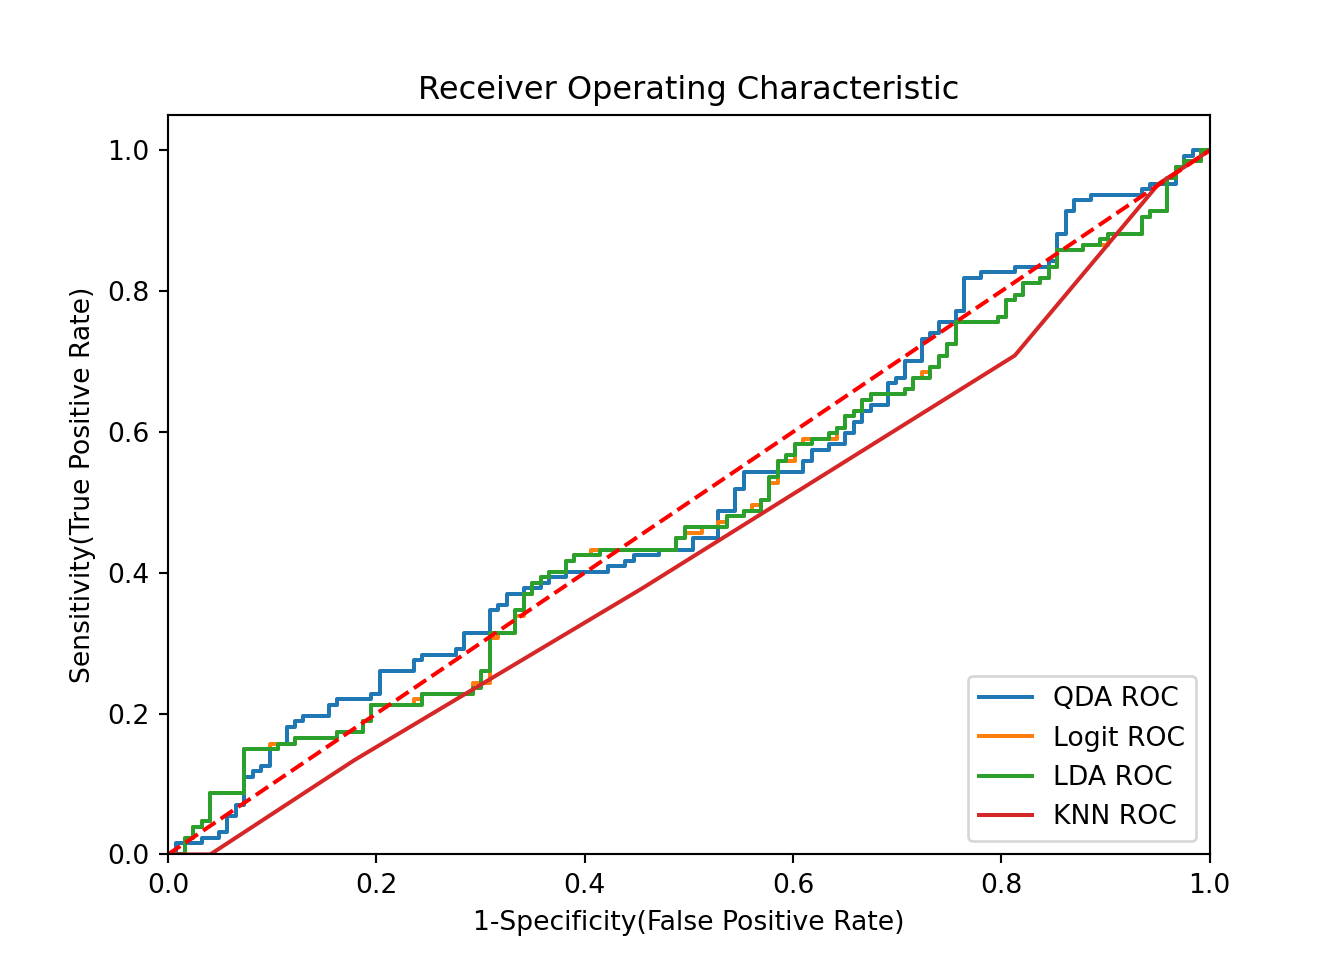
\includegraphics[keepaspectratio]{classification_files/figure-pdf/unnamed-chunk-18-1.pdf}}

So we plotting ROC-AUC curves. Generally we want it to look a lot better
than this. But this will give us a chance to talk about these. When it
comes to evaluating models ROC-AUC curves are a favorite. These
complement each other in a lot of respects.

In our accuracy, precision, recall, and F1 scores they all try to
evaluate the proportion of true positives in comparision to either total
classifications or something else. However, we don't really ever have a
good intuition at what level we should be cutting off these judgements.
ROC-AUC lets us plot the performance of our models at various thresholds
and against the random chance. In this case there are lots of instances
whwer our model is not even as good as the random classifier. We
probably need more features in order to improve our sensitivity.

In general we want it to look more curvy where the ROC-AUC is a lot
closer to the 1 on the Y axis. A flat curve indicates that our model
performs as well as flipping a coin. In any classification task we are
going to have some mistakes in classification no matter the threshold. A
AUC of 0.8 would indicate that our classifier is going to classify that
point correctly close to 80\% of the time.

\section{Getting Marginal effects}\label{getting-marginal-effects}

\bookmarksetup{startatroot}

\chapter{Tree Based Methods and an Aside on
Validation}\label{tree-based-methods-and-an-aside-on-validation}

For a variety of regression and classification tasks we can use what was
once the state of the art and that is random forrests

\begin{Shaded}
\begin{Highlighting}[]
\ImportTok{import}\NormalTok{ polars }\ImportTok{as}\NormalTok{ pl }
\ImportTok{import}\NormalTok{ polars.selectors }\ImportTok{as}\NormalTok{ cs}
\ImportTok{from}\NormalTok{ sklearn.datasets }\ImportTok{import}\NormalTok{ make\_regression}
\ImportTok{from}\NormalTok{ sklearn.ensemble }\ImportTok{import}\NormalTok{ GradientBoostingRegressor}
\ImportTok{import}\NormalTok{ numpy }\ImportTok{as}\NormalTok{ np}
\ImportTok{import}\NormalTok{ pandas }\ImportTok{as}\NormalTok{ pd }
\ImportTok{import}\NormalTok{ matplotlib.pyplot }\ImportTok{as}\NormalTok{ plt}
\ImportTok{from}\NormalTok{ sklearn }\ImportTok{import}\NormalTok{ tree}
\ImportTok{from}\NormalTok{ sklearn.tree }\ImportTok{import}\NormalTok{ (DecisionTreeClassifier }\ImportTok{as}\NormalTok{ DTC,}
\NormalTok{                          DecisionTreeRegressor }\ImportTok{as}\NormalTok{ DTR,}
\NormalTok{                          plot\_tree,}
\NormalTok{                          export\_text)}
\ImportTok{from}\NormalTok{ sklearn.metrics }\ImportTok{import}\NormalTok{ (accuracy\_score,}
\NormalTok{                             log\_loss)}
\ImportTok{from}\NormalTok{ sklearn.model\_selection }\ImportTok{import}\NormalTok{ train\_test\_split}
\ImportTok{from}\NormalTok{ sklearn.model\_selection }\ImportTok{import}\NormalTok{ cross\_val\_score}
\ImportTok{from}\NormalTok{ sklearn.metrics }\ImportTok{import}\NormalTok{ accuracy\_score, precision\_score, recall\_score, f1\_score, roc\_auc\_score, confusion\_matrix, classification\_report, ConfusionMatrixDisplay                            }
\ImportTok{from}\NormalTok{ sklearn.ensemble }\ImportTok{import} \OperatorTok{\textbackslash{}}
\NormalTok{     (RandomForestRegressor }\ImportTok{as}\NormalTok{ RF,}
\NormalTok{      GradientBoostingRegressor }\ImportTok{as}\NormalTok{ GBR)}
\ImportTok{import}\NormalTok{ pymc\_bart }\ImportTok{as}\NormalTok{ pmb}
\ImportTok{import}\NormalTok{ pymc }\ImportTok{as}\NormalTok{ pm }
\ImportTok{import}\NormalTok{ arviz }\ImportTok{as}\NormalTok{ az}


\NormalTok{carseats }\OperatorTok{=}\NormalTok{ pl.read\_csv(}\StringTok{\textquotesingle{}data/Carseats.csv\textquotesingle{}}\NormalTok{).with\_columns(}
\NormalTok{    pl.when(pl.col(}\StringTok{\textquotesingle{}Sales\textquotesingle{}}\NormalTok{) }\OperatorTok{\textgreater{}} \DecValTok{0}\NormalTok{).then(pl.lit(}\StringTok{\textquotesingle{}Yes\textquotesingle{}}\NormalTok{)).otherwise(pl.lit(}\StringTok{\textquotesingle{}No\textquotesingle{}}\NormalTok{)).alias(}\StringTok{\textquotesingle{}high\textquotesingle{}}\NormalTok{)}
\NormalTok{)}
\end{Highlighting}
\end{Shaded}

\section{A Tree}\label{a-tree}

Underriding the entire idea of random forests are regression trees.
Regression trees have a lot of math behind an inherently kind of simple
and beautifully dumb idea.

When we fit a single tree there are a set of rules that we give it to
make decisions about the data if a variable hits that rule then
depending on what side of the line it is then it will split the data off
into the left or right side. In the example above when income is not
greater than or equal to 24.5 we split it into the false category an
then it stops. We have satisfied the criteria. In the true column we
then repeat the proces however when we hit the false column again we
have a new criterion and that is how much there is on advertising
spending.

Formally we are splitting the predictor space into a number of regions
or leave or the little boxes. The branches, lines are the branches.
Somewhat unituitevely at first the leaves appear at the bottom and the
stem appears at the top. Intuitively each side gets labelled region one
on the graph with the associated points and so on and so forth. In
practice this creates a lot of weird boundaries that map onto
interactions or different functional forms. Making them good at finding
thse relationships without directly specifying them.

\section{Why do this?}\label{why-do-this}

OLS is really nice in the social sciences where we have a better
understanding of the DGP and not alot of variables. In a datascience we
don't neccessarily have that or have the luxury of a lot of data. One
thing that OLS does a poor job of is that we have to enter in the
relationships ourselves and every possible combination of interactions
or functional form of a small set of variables is going to overfit the
model/we are going to have a lot of multicollinearity. OLS has a closed
form solution where we are making these predictions over the entire
data. Which is going to get messy in a way we may not quite understand.

Regression trees divide the this mess into smaller regions. We are
effectively dividing up the space into small mutually exclusive regions.
We do this by starting off greedy we find some value that does well with
our splitting rule. Then it will make a split into a mutually exclusive
regions then redo this process. Instead of looking ahead to see if there
is some partiontion that will make its predictions better in the future
it will choose what is convenient.

\section{Gardening}\label{gardening}

As you may imagine growing a tree can maximize in sample fit but thats
not really what we are after. However a tree with two branches maybe
really interpretable and less sensitive to new data but is going to be
somewhat biased. In the regression part we did a little cross validation
but didn't really go over it so it is worth talking about.

Cross-validation is critical to our workflow. We use training and test
sets to evaluate our models. This is good but effectively we are only
evaluating our model once with the validation set. Instead of a spray
and pray approach we can hold out ``more'' data to evaluate our model
and tweak it. Generally we want a model that minimizes our test set
error. But if tweak the model based on the test set we are going to end
up overfitting. Effectively as I understand it is that we are getting
leakage into the training phase without cross-validation.

Cross-validation helps with this because we are using parts of our
training set that the model hasn't seen before to tune our models. We
shuffle the data a bit and then evaluate our model on the folds. There
are lots of methods most people use is K-fold cross validation. We
effectively create lots of datasets from our training set where some of
the data is used in the evaluation phase and some of it is used in the
training phase. This is really beneficial because you can't just wait
around for more data.

\section{Creating a Forest or Boosting a
Tree?}\label{creating-a-forest-or-boosting-a-tree}

As you may imagine striking a delicate balance in growing a single tree
is tricky. Basiscally trees are a little bit like adaptive nearest
neighbors. This gets a little more complicated but we will not get into
that to much. Once we start partition to things into finer and finer
neighborhoods we may be able to tune it pretty well but it is going to
be extremely sensitive. Enter bagging and boosting. These rely on a
similar idea but go about it in a different way. Basically what if we
just made a bunch of dumb models and found a way to make them not dumb?

\section{Bagging}\label{bagging}

Bagging is just a fancy way of saying voting or averaging. Instead of
one smart tree we make a bunch of them! We fit the trees on random parts
of our training data and penalize them for getting them to smart. Once
each tree makes its predictions we ask them to vote or average their
predictions. Whatever gets spit out is the answer to our problem.
Conditional on us doing it correctly. So in classification problem if we
are predicting whether or not a transaction is fraudulent we would fit
the model asking it to classify a bunch of transactions as fraud or not.
Whatever number of trees we ask it to make we are just going to take a
simple vote on whether that transaction is fraud or not. It is a little
beautifully democratic. This works because we are using the predictions
from sevearl weak learners where we have high variance but low bias.
Meaning that we may not always get our darts in the same area but the
difference between predicted and real values is low. Then once we
average over these weak learners we reduce our variance.

Random forests are based off of this idea but we add a small tweak. We
still fit a large number of bad learners but we decorrelate the trees to
improve performance. We sample the data with replacement where some
trees see the same information a few times while others never see the
same inforamtion. We also never let any one tree see a majority of the
predictors. This will bias downward really good predictors and give
other predictors a chance. Than we take a vote/average of what the trees
spit out.

\section{Boosting}\label{boosting}

Our other option is boosting. Boosting has different mechanics but the
same idea. Instead of making a really good tree we start with a tree
that slightly better than random guessing but not that much better on
some sample of our training data. However, instead of modeling a lot of
trees at once we sequentially fit a series of tree. However, we
substitute in the residuals from the prior model as the starting point.
There are a few ways to do this the most popular methods are adaboost
and gradient boosting. They have a similar idea but go about it in
different ways.

\subsection{Adaboost}\label{adaboost}

ADAboost focuses on the misclassification part. Where we take the
residuals of the weak learners then re-weight the samples to give more
weight to mistakes. Then at the end we take the contribution of each
learner as the weighted average of the predictions/majority vote. This
was popular for awhille but tends not to perform that well compared to
gradient boosting.

\subsection{Gradient Boosting}\label{gradient-boosting}

Instead of focusing on the misclassifications as the starting point we
are minimizing some loss function. What is annoying about machine
learning is that they are always coming up with catchier terms for old
concepts. By gradient we are really just talking about a vector of
partial derivatives of a model's parameters. In particular the learning
rate and leaf node values point gradient descent in the write direction
meaning that we are decreasing the loss the fasted. The difference
between the predicitions and the actual value effectively tell the other
trees what ``direction'' to go to minimize the loss function.

\begin{Shaded}
\begin{Highlighting}[]
\NormalTok{X, y }\OperatorTok{=}\NormalTok{ make\_regression(n\_samples}\OperatorTok{=}\DecValTok{100}\NormalTok{, n\_features}\OperatorTok{=}\DecValTok{1}\NormalTok{, noise}\OperatorTok{=}\DecValTok{10}\NormalTok{, random\_state}\OperatorTok{=}\DecValTok{42}\NormalTok{)}
\NormalTok{gbr }\OperatorTok{=}\NormalTok{ GradientBoostingRegressor(n\_estimators}\OperatorTok{=}\DecValTok{5}\NormalTok{, learning\_rate}\OperatorTok{=}\FloatTok{0.1}\NormalTok{, max\_depth}\OperatorTok{=}\DecValTok{2}\NormalTok{, random\_state}\OperatorTok{=}\DecValTok{42}\NormalTok{)}
\NormalTok{gbr.fit(X, y)}
\NormalTok{stage\_predictions }\OperatorTok{=}\NormalTok{ np.array(}\BuiltInTok{list}\NormalTok{(gbr.staged\_predict(X)))}

\NormalTok{colors }\OperatorTok{=}\NormalTok{ [}\StringTok{\textquotesingle{}red\textquotesingle{}}\NormalTok{, }\StringTok{\textquotesingle{}green\textquotesingle{}}\NormalTok{, }\StringTok{\textquotesingle{}blue\textquotesingle{}}\NormalTok{, }\StringTok{\textquotesingle{}orange\textquotesingle{}}\NormalTok{, }\StringTok{\textquotesingle{}purple\textquotesingle{}}\NormalTok{]}

\CommentTok{\# Plot predictions from each tree}
\NormalTok{plt.figure(figsize}\OperatorTok{=}\NormalTok{(}\DecValTok{10}\NormalTok{, }\DecValTok{6}\NormalTok{))}
\ControlFlowTok{for}\NormalTok{ i, preds }\KeywordTok{in} \BuiltInTok{enumerate}\NormalTok{(stage\_predictions):}
\NormalTok{    plt.scatter(X, y, label}\OperatorTok{=}\StringTok{\textquotesingle{}True Data\textquotesingle{}}\NormalTok{, color}\OperatorTok{=}\StringTok{\textquotesingle{}blue\textquotesingle{}}\NormalTok{, alpha}\OperatorTok{=}\FloatTok{0.3}\NormalTok{)  }\CommentTok{\# True data is blue}
\NormalTok{    plt.scatter(X, preds, label}\OperatorTok{=}\SpecialStringTok{f\textquotesingle{}Tree }\SpecialCharTok{\{}\NormalTok{i}\OperatorTok{+}\DecValTok{1}\SpecialCharTok{\}}\SpecialStringTok{ Predictions\textquotesingle{}}\NormalTok{, color}\OperatorTok{=}\NormalTok{colors[i], alpha}\OperatorTok{=}\FloatTok{0.6}\NormalTok{)  }\CommentTok{\# Different colors for each tree}
\NormalTok{    plt.title(}\SpecialStringTok{f"After Tree }\SpecialCharTok{\{}\NormalTok{i}\OperatorTok{+}\DecValTok{1}\SpecialCharTok{\}}\SpecialStringTok{"}\NormalTok{)}
\NormalTok{    plt.xlabel(}\StringTok{"Feature"}\NormalTok{)}
\NormalTok{    plt.ylabel(}\StringTok{"Target"}\NormalTok{)}
    
    \CommentTok{\# Calculate residuals after this tree\textquotesingle{}s prediction}
\NormalTok{    residuals }\OperatorTok{=}\NormalTok{ y }\OperatorTok{{-}}\NormalTok{ preds}
    \BuiltInTok{print}\NormalTok{(}\SpecialStringTok{f"Residuals after Tree }\SpecialCharTok{\{}\NormalTok{i}\OperatorTok{+}\DecValTok{1}\SpecialCharTok{\}}\SpecialStringTok{: }\SpecialCharTok{\{}\NormalTok{residuals[:}\DecValTok{5}\NormalTok{]}\SpecialCharTok{\}}\SpecialStringTok{"}\NormalTok{)}

\CommentTok{\# Move legend outside the plot}
\NormalTok{plt.legend(loc}\OperatorTok{=}\StringTok{\textquotesingle{}upper left\textquotesingle{}}\NormalTok{, bbox\_to\_anchor}\OperatorTok{=}\NormalTok{(}\DecValTok{1}\NormalTok{, }\DecValTok{1}\NormalTok{), title}\OperatorTok{=}\StringTok{"Legend"}\NormalTok{)}

\NormalTok{plt.tight\_layout()  }\CommentTok{\# Adjust layout to fit the legend outside}
\NormalTok{plt.show()}
\end{Highlighting}
\end{Shaded}

\begin{verbatim}
Residuals after Tree 1: [ 48.50379764  -7.99162897 -29.48721169  12.60038417 -12.30719702]
Residuals after Tree 2: [ 43.43590543  -8.74058441 -26.77902107  11.85142874  -9.5990064 ]
Residuals after Tree 3: [ 38.69686574  -9.94190283 -25.21365705  10.65011032  -8.03364238]
Residuals after Tree 4: [ 36.45100414  -9.51962888 -21.24402815   8.40424871  -7.61136843]
Residuals after Tree 5: [ 32.76894548 -10.04360784 -19.28355557   7.88026975  -5.65089585]
\end{verbatim}

\pandocbounded{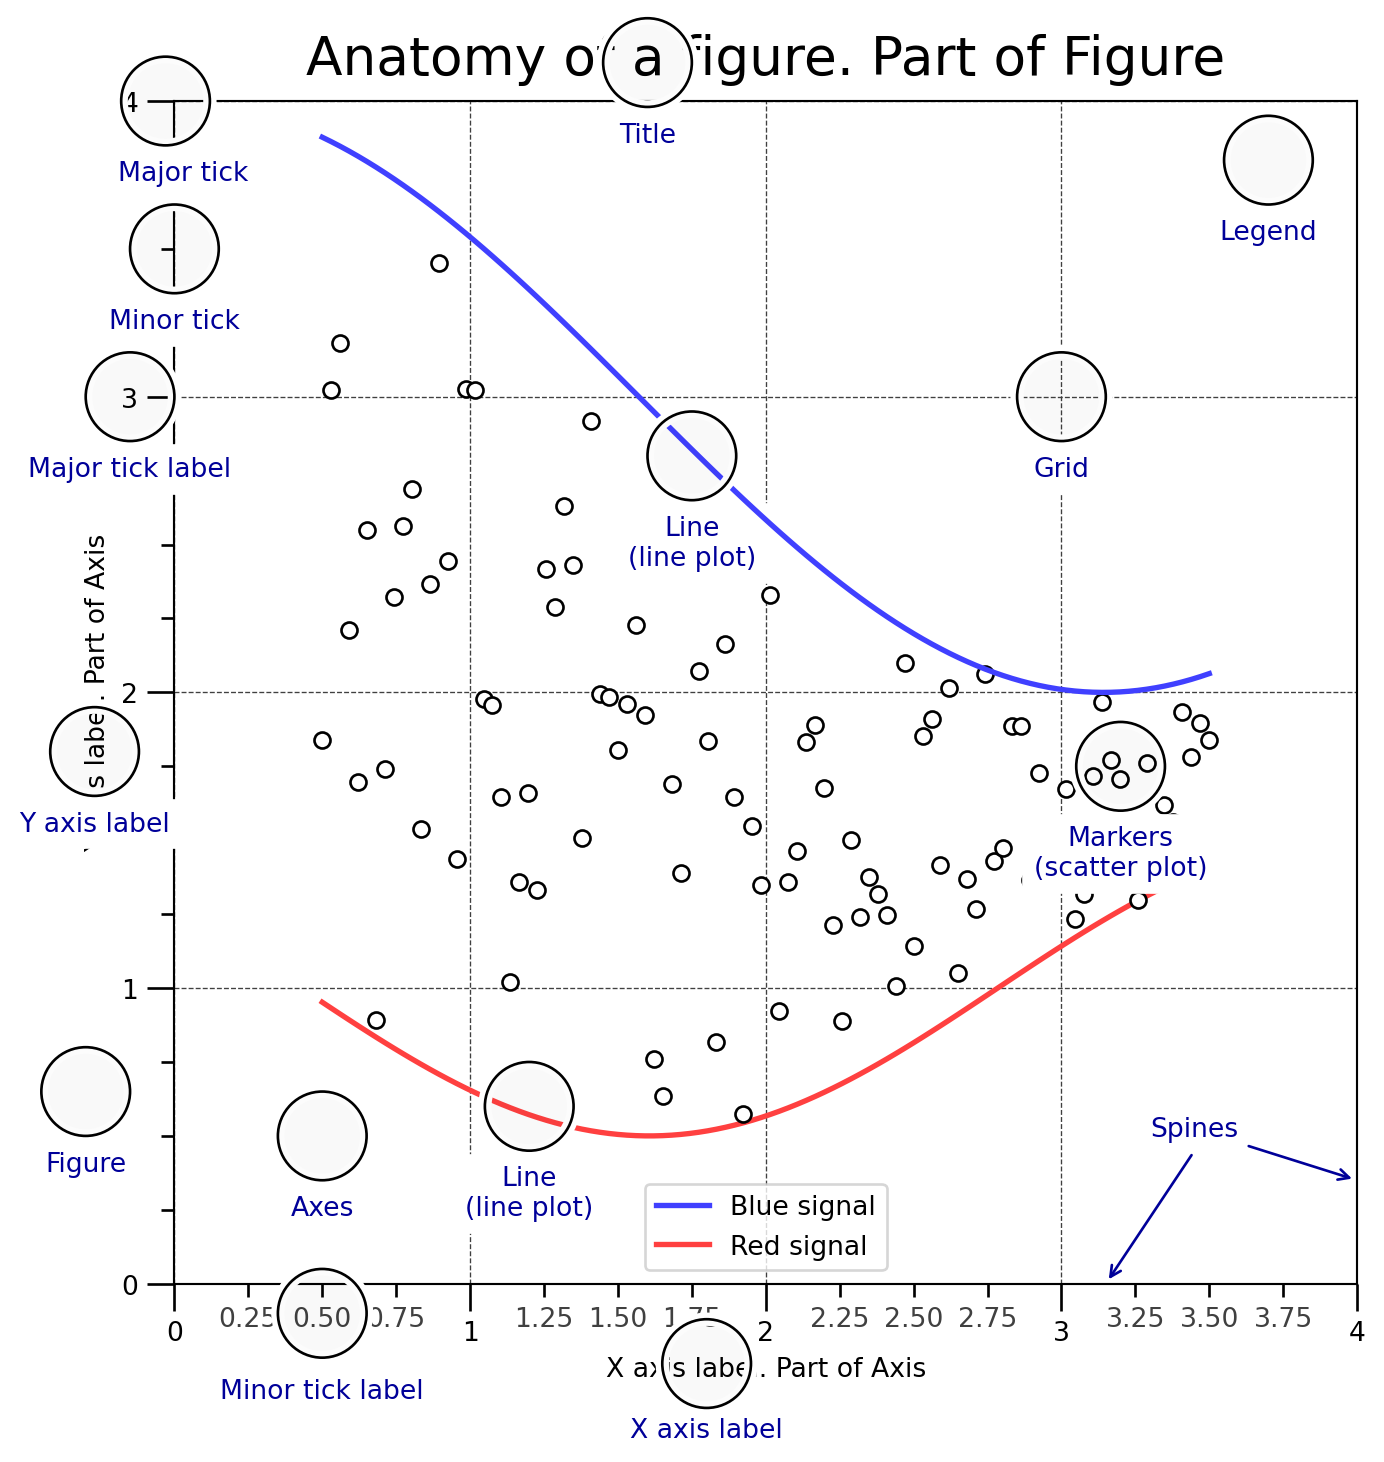
\includegraphics[keepaspectratio]{tree-based-methods_files/figure-pdf/cell-3-output-2.pdf}}

Within the gradient boosting framework we have two popular approaches:
XGboost and LightGBM. Each of these approaches focus on impurity meaning
how well a tree can distinguish between two classes using something like
a GINI coeficient or Entropy that tries to measure class separtion or
using mean squared error.

They both work to reduce these impurities however they differ in how
they grow the tree. LightGbm focuses on the leaf wise growth whereas
xgboost will do branch or level wise growth. Functionally all this means
is that for a level wise strategy we are growing both sides of the flow
chart which kind of imposes some regularization. Whereas leafwise growth
adds more and more leaves making better predictions but is prone to
overfitting.

\section{Gradient Boosting or Random
Trees}\label{gradient-boosting-or-random-trees}

The answer is that it kind of depends. Gradient boosting of what ever
flavor you choose is going to be more prone to overfitting that random
forests. Gradient boosting is also a little bit better in the face of
class imbalances. Since the prior tree is used to inform the previous
tree if you don't select good features in the beginning you could end of
fitting the noise. The other problem is compute time. Since gradient
boosting relies on the previous tree it has to wait till that tree is
done being fit.

\bookmarksetup{startatroot}

\chapter{Unsupervised Learning}\label{unsupervised-learning}

In the prior ``chapters'' we covered a variety of supervised learning
techniques. By supervised we have some direct control over
hyperparameter tuning and how we enter things into the model to predict
a response. Unsupervised learning doesn't neccessarily have a dependent
variable that we are trying to predict. Instead the unsupervised
techniques covered in ISLR and ESLR look at unsupervised learning as an
approach to help us uncover hidden groups in our data. They focus on PCA
and various clustering methods. There are no hard and fast rules with
this and we often think of it as an EDA excercise or a way to reduce the
dimensionality of our data. In effect supervised learning is learning
the relationship of data without labels. So say we need to build a
classifier. We label the data as penguin not a penguin without then we
train a model on these things. For an unsupervised model we may not care
so much but may want to throw everything in a model and then see if the
model can uncover groupings of penguin not penguin.

\section{The Curse}\label{the-curse}

The curse of dimensionality frequently comes up in machine learning
because we often have a ton of predictors. The curse of dimensionality
can be a little weird if you don't deal with math a whole lot. The
general idea of the curse of dimensionality is that as the number of
dimensions increase our models are going to start to break down because
as the number of dimensions increase our model is going to find data
points standing all alone. We may not know that because our model starts
to do well finding things that are alone in a neighborhood. A good model
will be able to find these points hiding in a crowd a bad model
wouldn't! Both good and bad models will find points by themselves which
is not neccessarily helpful as we start to introduce new data points the
model's performance will start to detoriate.

The thing with the curse of dimensionality is that we never escape it
because we are going to run into when modeling variables. For OLS the
curse of dimensionality enters as we start to add more and more
variables because we are stratiying our data by more and more
information. Even when we are doing something like inverse propensity
score weighting and then using these weights in a bivariate OLS you are
running into the curse in the propensity score equation.

\section{What can we do about the
curse?}\label{what-can-we-do-about-the-curse}

We can use methods like PCA to reduce the number of dimensions. The
general idea is that we are trying to map high dimensional relationships
into lower dimesional proxies.

\begin{Shaded}
\begin{Highlighting}[]
\ImportTok{import}\NormalTok{ polars }\ImportTok{as}\NormalTok{ pl}
\ImportTok{import}\NormalTok{ polars.selectors }\ImportTok{as}\NormalTok{ cs }
\ImportTok{import}\NormalTok{ matplotlib.pyplot }\ImportTok{as}\NormalTok{ plt}
\ImportTok{from}\NormalTok{ palmerpenguins }\ImportTok{import}\NormalTok{ load\_penguins}

\NormalTok{pengs }\OperatorTok{=}\NormalTok{ pl.from\_pandas(load\_penguins())}

\NormalTok{pengs.select(pl.exclude(}\StringTok{\textquotesingle{}year\textquotesingle{}}\NormalTok{, }\StringTok{\textquotesingle{}species\textquotesingle{}}\NormalTok{, }\StringTok{\textquotesingle{}sex\textquotesingle{}}\NormalTok{, }\StringTok{\textquotesingle{}island\textquotesingle{}}\NormalTok{)).drop\_nans().corr()}
\end{Highlighting}
\end{Shaded}

\begin{longtable}[]{@{}llll@{}}
\toprule\noalign{}
bill\_length\_mm & bill\_depth\_mm & flipper\_length\_mm &
body\_mass\_g \\
f64 & f64 & f64 & f64 \\
\midrule\noalign{}
\endhead
\bottomrule\noalign{}
\endlastfoot
1.0 & -0.235053 & 0.656181 & 0.59511 \\
-0.235053 & 1.0 & -0.583851 & -0.471916 \\
0.656181 & -0.583851 & 1.0 & 0.871202 \\
0.59511 & -0.471916 & 0.871202 & 1.0 \\
\end{longtable}

Each of these variables map on to some measure of penguin bigness some
of them are more correlated with each other but if we had flipper width
or bill width or some other measure of penguins bigness there is going
to significant overlap. Once we enter these into a regression these
models are going to pretty good job at descrbing penguin weirdness. A
way to help us is to summarize these variables into what we call
principal components.

Principal components are a way to summarize the variation in these
overlapping variables in a minimal set of variables.

\begin{Shaded}
\begin{Highlighting}[]
\ImportTok{from}\NormalTok{ sklearn.decomposition }\ImportTok{import}\NormalTok{ PCA}

\NormalTok{normalized }\OperatorTok{=}\NormalTok{ pengs.select(cs.numeric(), pl.col(}\StringTok{\textquotesingle{}species\textquotesingle{}}\NormalTok{)).select(pl.exclude(}\StringTok{\textquotesingle{}year\textquotesingle{}}\NormalTok{)).with\_columns(}
\NormalTok{        (cs.numeric() }\OperatorTok{{-}}\NormalTok{ cs.numeric().mean() }\OperatorTok{/}\NormalTok{ cs.numeric().std())}
\NormalTok{    ).drop\_nulls()}

\NormalTok{pca }\OperatorTok{=}\NormalTok{ PCA()}
\NormalTok{numeric\_data }\OperatorTok{=}\NormalTok{ normalized.select(cs.numeric())}
\NormalTok{pca.fit(numeric\_data)}

\CommentTok{\# Transform the data and include species labels}
\NormalTok{tr\_df }\OperatorTok{=}\NormalTok{ pca.transform(numeric\_data)}
\NormalTok{pca\_components }\OperatorTok{=}\NormalTok{ pl.DataFrame(}
\NormalTok{    tr\_df,}
\NormalTok{    schema}\OperatorTok{=}\NormalTok{[}\SpecialStringTok{f\textquotesingle{}PC}\SpecialCharTok{\{}\NormalTok{i}\OperatorTok{+}\DecValTok{1}\SpecialCharTok{\}}\SpecialStringTok{\textquotesingle{}} \ControlFlowTok{for}\NormalTok{ i }\KeywordTok{in} \BuiltInTok{range}\NormalTok{(tr\_df.shape[}\DecValTok{1}\NormalTok{])]}
\NormalTok{).with\_columns(normalized[}\StringTok{\textquotesingle{}species\textquotesingle{}}\NormalTok{]) }

\NormalTok{pca\_df }\OperatorTok{=}\NormalTok{ pca\_components.to\_pandas()}

\CommentTok{\# Define a color map for the species}
\NormalTok{color\_map }\OperatorTok{=}\NormalTok{ \{}
    \StringTok{"Adelie"}\NormalTok{: }\StringTok{"red"}\NormalTok{,}
    \StringTok{"Gentoo"}\NormalTok{: }\StringTok{"blue"}\NormalTok{,}
    \StringTok{"Chinstrap"}\NormalTok{: }\StringTok{"green"}
\NormalTok{\}}

\CommentTok{\# Create the scatter plot}
\NormalTok{plt.figure(figsize}\OperatorTok{=}\NormalTok{(}\DecValTok{8}\NormalTok{, }\DecValTok{6}\NormalTok{))}
\ControlFlowTok{for}\NormalTok{ species, color }\KeywordTok{in}\NormalTok{ color\_map.items():}
\NormalTok{    subset }\OperatorTok{=}\NormalTok{ pca\_df[pca\_df[}\StringTok{\textquotesingle{}species\textquotesingle{}}\NormalTok{] }\OperatorTok{==}\NormalTok{ species]}
\NormalTok{    plt.scatter(}
\NormalTok{        subset[}\StringTok{\textquotesingle{}PC1\textquotesingle{}}\NormalTok{], }
\NormalTok{        subset[}\StringTok{\textquotesingle{}PC2\textquotesingle{}}\NormalTok{], }
\NormalTok{        label}\OperatorTok{=}\NormalTok{species, }
\NormalTok{        color}\OperatorTok{=}\NormalTok{color, }
\NormalTok{        alpha}\OperatorTok{=}\FloatTok{0.7}
\NormalTok{    )}

\CommentTok{\# Add plot details}
\NormalTok{plt.title(}\StringTok{\textquotesingle{}PCA: First Two Principal Components\textquotesingle{}}\NormalTok{)}
\NormalTok{plt.xlabel(}\StringTok{\textquotesingle{}Principal Component 1\textquotesingle{}}\NormalTok{)}
\NormalTok{plt.ylabel(}\StringTok{\textquotesingle{}Principal Component 2\textquotesingle{}}\NormalTok{)}
\NormalTok{plt.legend(title}\OperatorTok{=}\StringTok{\textquotesingle{}Species\textquotesingle{}}\NormalTok{)}
\NormalTok{plt.grid()}
\NormalTok{plt.show()}
\end{Highlighting}
\end{Shaded}

\pandocbounded{\includegraphics[keepaspectratio]{unsupervised-learning_files/figure-pdf/cell-3-output-1.pdf}}

We can see that these two variables do a reasonable enough job of
distinguishing the species from each other. What is going on underneath
the hood is that we are creating some linear combinations of these
variables. We can relax this constraint using gams if we want but in
practice we do this linearly alot.

\section{Clustering}\label{clustering}

In a sense we are finding subgroups with this PCA example but we can
also use clustering algorithms. Basically clustering algorithms will try
to ifer subgroups from the data either through minimizing a distance
measure if we are using k-means. We could also use mixture clustering
where we make some assumptions of the distributions but can let more
moment conditions enter into the clustering algorithm.

\bookmarksetup{startatroot}

\chapter{Time-Series}\label{time-series}

Time is something that we all have to deal with. The problem with time
in statistics is that it is SUPER SUPER finnicky. When we start to model
a single thing over time much less multiple things shit starts to get
weird really quickly. So lets get back into your time series notes.

\section{Why Bother?}\label{why-bother}

Generally we have some fixes when linear regression starts to break
down. The problem is that they only go so far and are not neccessarily
going to gain us that much insightful leverage on the data generating
proces. As lots of articles argue. We should take time seriously! So how
do we do that?

We have several families of Time Series methods:

\begin{enumerate}
\def\labelenumi{\arabic{enumi}.}
\tightlist
\item
  Error Correction Models
\item
  ARIMA
\item
  ARCH/GARCH
\item
  GAMS
\item
  Machine Learning Stuff
\end{enumerate}

Traditionally in Political Science and Economics we tend to focus on the
first 3. There are some that you are just not going to run into much in
the wild in political science but are worth learning about since you are
probably going to be pushed to use them.

\section{Dynamic Regression}\label{dynamic-regression}

Lets focus on the crux of the issue when we are thinking about time
series. Lets say we are interested in modeling the relationship spending
and selling over time. Our naive smooth brain may tell us that we should
model it like this.

\[
\text{Spending} = \alpha_{t} + \beta_{t} \text{income} + \varepsilon{t}
\]

This would be fine if we only had one time point! But as we start to add
time points previous values of spending are going to tell us about
future values of spending same with prior values of income. This
violates our autocorrelation assumption. What ends up happening is that
we can correctly estimate the slope of the regression line but our
standard errors will be off. The reason this happens is that the
standard error is normally calculated by taking a weighted mean of the
deviations of the observed yi. What then ends up happening with this
calaculation is that we are kind of adding the previous periods error
plus the autoregressive order. We could theoretically correct our
standard errors. However, we tend to over reject the null and the use of
standard error corrections in this setting tend to point toward bigger
problems beneath the surface. In our model we are kind of saying that
only contemporaneous values income are the only thing that matters. What
is likely the true model is something along the lines of

\[
\text{Spending} = \alpha_{0} + \alpha_{1} \text{Spending}_{t-1} + \beta_1 Income_{t} + \varepsilon_{t}
\]

What this implies is that our model cross sectional model is wrong
because we are leaving the lag of y out of the model. Something that
will propagate in our model. What this means is that \(Spending_{t-1}\)
is going to be related to contemporaneous spending and our estimates
will be unbiased and inconsistent kind of no matter what we do.

\phantomsection\label{refs}
\begin{CSLReferences}{1}{0}
\bibitem[\citeproctext]{ref-lundbergWhatYourEstimand2021}
Lundberg, Ian, Rebecca Johnson, and Brandon M. Stewart. 2021. {``What
{Is Your Estimand}? {Defining} the {Target Quantity Connects Statistical
Evidence} to {Theory}.''} \emph{American Sociological Review} 86 (3):
532--65. \url{https://doi.org/10.1177/00031224211004187}.

\end{CSLReferences}




\end{document}
